\part{Global methods for sampling rare diffusive events}

\chapter{Ritz methods for Freidlin-Wentzel-Graham actions} \label{ch:Ritz methods for Freidlin-Wentzel-Graham actions}

\section{Introduction}

The theory of Freidlin and Wentzell \citep{ventsel1970small}
gives asymptotic probability estimates of rare events in dynamical
systems perturbed by small noise \citep{bolhuis2002transition, allen2005sampling, allen2009forward, ebener2019instanton}.
Specifically, Freidlin-Wentzell theory yields estimates of the stationary
distributions and mean first-passage times. Both these quantities
are determined, in turn, by the asymptotic estimate of the probability
of a stochastic trajectory to not deviate from a smooth path by more
than a given amount in a given interval of time. The key result of
Freidlin and Wentzell is that the limiting form of this probability,
for small noise and small deviations, is given by a non-negative functional
of the smooth path. This functional is the Freidlin-Wentzell action
and its minimum, for fixed initial and terminal states, determines
both the stationary distributions and first-passage times. The smooth
path minimising the action is often called the Freidlin-Wentzell instanton.
The theory is applicable to dynamical systems of both gradient and
non-gradient character and can so be used to study a wide variety
of equilibrium and non-equilibrium systems modelled by Itô diffusions
\citep{paninski2006most,huang2012molecular, bouchet2016generalisation, maier1996scaling, wolynes1995navigating, nolting2016balls, mangel1994barrier, gardner2000construction, demarco2001phase, nelson1987stochastic}.

Determining the minimum of the Freidlin-Wentzell action is a problem
in the calculus of variations. The Euler-Lagrange equations provide
the necessary conditions for extrema of variational problems and,
unsurprisingly, have been the basis of the large literature devoted
to the numerical computation of Freidlin-Wentzell instantons \citep{weinan2002string,paninski2006most,heymann2008geometric,grafke2017long}.
There exists, however, an alternative ``direct'' route for the solution
of variational problems in which the functional is reduced, through
finite-dimensional parametrizations of paths, to a multivariate function
and then extre\textcolor{black}{mised by appropriate multivariate
optimisation methods \citep{gelfand2012calculus,kantorovich1958approximate}.
To the best of our knowledge, the first use of the direct method for
the Freidlin-Wentzell action, discretised by finite-differences, appears
in the work of Weinan, Ren and Vanden-Eijnden \citep{weinan2004minimum}.} 

Here we combine the direct method with a Ritz discretisation \citep{ritz1909uber,gelfand2012calculus,kantorovich1958approximate}
to minimize the Freidlin-Wentzell action. We analyse paths in a spectral
basis of Chebyshev polynomials and use spectral quadrature to express
the action as a multivariate function of the basis coefficients. Nonlinear
optimisation is used to obtain coefficients that give the least action
from which the instanton is synthesised in the spectral basis.\textcolor{black}{{}
For minimisation over paths regardless of their duration, this procedure
is especially effective when applied to a reparametrisation-invariant
on-shell form of the action that follows from the time-translational
invariance of the Lagrangian. This generalises the scalar work functional
of Olender and Elber (for gradient dynamics) and the geometric action
of Heyman and Vanden-Eijnden} \citep{vanden2008geometric} (for non-gradient
dynamics). Our method is efficient enough to robustly sample the logarithm
of the asymptotic estimate of the stationary distribution, \emph{i.e.
}the quasipotential, avoiding the alternative, but numerically delicate,
route of solving the Hamilton-Jacobi equation \citep{cameron2012finding,yang2019computing,dahiya2018ordered}.
Our method is simple to use, converges rapidly, and is applicable
to both equilibrium and non-equilibrium problems. Its implementation
is freely available on GitHub as the open-source Python library PyRitz. 

The remainder of this chapter is organized as follows. In the next section,
we recall key results of Freidlin-Wentzell theory from dual perspectives
of Itô stochastic differential equations and the corresponding Fokker-Planck
equations.\textcolor{black}{{} Sec.~\ref{sec:Minima-of-the-action}
we present the derivation of the on-shell form of the Freidlin-Wentzell
action in a manner reminiscent of the Routh reduction procedure in
classical mechanics and explain its relation to the scalar work and
the geometric action. }In Sec.~\ref{sec:direct-method} we describe
the direct method for the minimisation of functionals, the Chebyshev
spectral basis in which we construct smooth paths, the spectral quadrature
rule we use to evaluate the action, and the multivariate non-linear
optimisation methods we employ to find the minimum. In Sec.~\ref{sec:pyritz-applications}
we apply the direct method to three well-known diffusion processes
and demonstrate convergence in each case. 

A particular achievement of our approach is its relatively facile
ability to calculate quasipotentials. This can be done with a sufficiently
high density of sample points to construct effectively continuous
maps of the quasipotential, which we do here for the same set of benchmark
problems. We conclude with a discussion on extending the method to
degenerate diffusion processes, systems with inertia and to the stochastic
dynamics of fields. 

\section{Large deviation theory} \label{sec:fwtheory}

We consider the autonomous dynamics of a $d$-dimensional coordinate
$X=(X^{1},\ldots,X^{d})$ in $\mathbb{R}^{d}$ perturbed by configuration-dependent
noise of intensity $\sqrt{\varepsilon}$ described by the Itô diffusion
equation \citep{oksendalStochasticDifferentialEquations2003, shreveStochasticCalculusFinance2005}
\begin{equation}
dX^{\mu}=a^{\mu}(X)dt+\sqrt{\varepsilon}\sigma_{\nu}^{\mu}(X)dW^{\nu}\label{general ito diffusion}
\end{equation}
governing the stochastic trajectory $X(t)$, where $a^{\mu}(X)$ is
the drift vector, $\sqrt{\varepsilon}\sigma_{\nu}^{\mu}(X)$ is the
volatility, $W^{\nu}(t)$ is a $d$-dimensional Wiener process and
repeated indices are summed over.  Eq.~\ref{general ito diffusion} is also often referred to as an \textit{overdamped Langevin equation}.

The transition probability density
of the process, $P_{1|1}(x,t|x_{0})=P(X(t)=x|X(0)=x_{0})$, obeys
the Fokker-Planck equation $\partial_{t}P(x|x_{0})=\mathcal{L}P(x|x_{0})$
where the Fokker-Planck operator is

\emph{
\begin{equation}
\begin{aligned}\mathcal{L}(x) & =-\frac{\partial}{\partial x^{\mu}}a^{\mu}(x)+\frac{\varepsilon}{2}\frac{\partial^{2}}{\partial x^{\mu}\partial x^{\nu}}b^{\mu\nu}(x)\end{aligned}
\label{eq:fokker-planck}
\end{equation}
}and \textbf{$b^{\mu\nu}(x)=\sigma_{\lambda}^{\mu}(x)\sigma_{\sigma}^{\nu}(x)\delta^{\lambda\sigma}$}
is the diffusion tensor. We assume it to be non-degenerate, positive-definite
and invertible. The inverse, $b_{\mu\nu}(x)$, induces a Riemannian
structure in $\mathbb{R}^{d}$ with a norm $|x|_{b}=\sqrt{b_{\mu\nu}x^{\mu}x^{\nu}}$
that is distinct from the Euclidean norm $|x|=\sqrt{(x^{1})^{2}+\ldots(x^{d})^{2}}.$
We use the subscript $b$ to indicate this second ``diffusion''
norm. The stationary density satisfies the time-independent Fokker-Planck
equation\emph{ }$\mathcal{L}P_{1}(x)=0$ and, when it exists, is reached
asymptotically in time for arbitrary initial distributions, $\lim_{t\rightarrow\infty}P_{1|1}(x,t|x_{0})=P_{1}(x)$.
The stationary distribution is unique for ergodic
systems \citep{pavliotis2014stochastic}. 

Associated with the Itô process is the Freidlin-Wentzell ``action''
functional \citep{ventsel1970small,graham1973statistical,graham1987macroscopic}
\begin{equation}
S[x(t)]=\frac{1}{2}\int_{0}^{T}|\dot{x}-a(x)|_{b}^{2}dt\label{eq:Freidlin-Wentzell action}
\end{equation}
which gives an asymptotic estimate for the logarithm of the probability
of trajectories $X(t)$ to remain in the tubular neighbourhood of
a smooth path $x(t)$ over the duration $0\le t\leq T$. We write
this as
\begin{equation}
P_{\text{tube}}[x(t)]\asymp\exp\left(-\frac{1}{\varepsilon}S[x(t)]\right)\label{eq:FW-LDP}
\end{equation}
which, in terms of limits, means

\[
S[x(t)]=\lim_{\delta\to0}\lim_{\varepsilon\to0}-\varepsilon\ln P\left[\sup_{0\leq t\leq T}|X(t)-x(t)|_{b}<\delta\right].
\]
The limits must be taken in the order above as they do not commute.
Eq.~\ref{eq:FW-LDP} is a large deviation principle for trajectories
of Itô processes, due to Wentzell and Freidlin and Graham \citep{touchette2009large}.

For reasons described below, it is of interest to obtain the mode
of the tube probability over the set of continuous paths
\[
\gamma_{T}=\{x(t)\,|\,x(0)=x_{1},x(T)=x_{2},0\leq t\leq T)\}
\]
which have fixed termini $x_{1}$ and $x_{2}$ and are of duration
$T.$ This is equivalent to the variational problem of minimising
the Freidlin-Wentzell action. The minimum value of the action,

\begin{equation}
V_{T}(x_{2}|x_{1})=\min_{\gamma_{T}}S[x(t)],
\end{equation}
is called the quasipotential. The path attaining the minimum,

\begin{equation}
x_{T}^{*}(t)=\arg\,\min_{\gamma_{T}}\,S[x(t)],
\end{equation}
is called the instanton. We emphasise that this path describes the
smooth centerline of the tube of maximum probability and not a non-differentiable
trajectory of the diffusion process. It is the most probable dynamical
path connecting two points in configuration space. 

The instanton and the quasipotential are central objects in Freidlin-Wentzell-Graham
theory and relate to the eikonal approximation of the Fokker-Planck
equation \citep{ludwig1975persistence}. Assuming the JWKB form of
the transition density,
\[
P_{1|1}(x,t|x_{0})\sim\exp\left[\frac{1}{\varepsilon}\sum_{n=0}^{\infty}\varepsilon^{n}\phi_{n}(x,x_{0};t)\right],
\]
with prefactors suppressed, substituting in the Fokker-Planck equation
and matching terms gives a Hamilton-Jacobi equation for the lowest
order contribution,
\begin{equation}
\partial_{t}\phi_{0}+\frac{1}{2}b^{\mu\nu}\partial_{\mu}\partial_{\nu}\phi_{0}+a^{\mu}\partial_{\mu}\phi_{0}=0.
\end{equation}
This corresponds to the Hamiltonian system
\begin{align}
H(x,p) & =\frac{1}{2}b^{\mu\nu}p_{\mu}p_{\nu}+a^{\mu}p_{\mu}\\
\dot{x}^{\mu} & =+\frac{\partial H}{\partial p_{\mu}}=b^{\mu\nu}p_{\nu}+a^{\mu}\nonumber \\
\dot{p}_{\mu} & =-\frac{\partial H}{\partial x^{\mu}}=-\frac{\partial b^{\nu\lambda}}{\partial x^{\mu}}p_{\nu}p_{\lambda}-\frac{\partial a^{\nu}}{\partial x^{\mu}}p_{\nu}\nonumber 
\end{align}
whose solutions define an equivalent variational problem of extremising
an action with the Lagrangian

\begin{align}
L(x,\dot{x}) & =p_{\mu}\dot{x}^{\mu}-H(x,p)\label{eq:Legendre-form-of-Lagrangian}\\
 & =\frac{1}{2}(\dot{x}^{\mu}-a^{\mu})b_{\mu\nu}(\dot{x}^{\nu}-a^{\nu}).\nonumber \\
 & =\frac{1}{2}|\dot{x}-a(x)|_{b}^{2}\nonumber 
\end{align}
Thus, the rays of the Hamilton-Jacobi equation that determine the
lowest order contribution to the eikonal are local maxima of the tube
probability, or in other words, $\phi_{0}(x,x_{0};T)=V_{T}(x|x_{0})$.
The large-deviation principle of Freidlin and Wentzell and the theory
of the non-equilibrium potential of Graham \citep{graham1973statistical,graham1987macroscopic}
thus appear as elegant reformulations of the JWKB approximation \citep{ludwig1975persistence}. 

The correspondence with the JWKB approximation yields the asymptotic
form of the transition density,
\begin{equation}
P_{1|1}(x,T|x_{0})\asymp\exp\left[-\frac{1}{\varepsilon}V_{T}(x|x_{0})\right],
\end{equation}
and, in the $T\rightarrow\infty$ limit of the above, the asymptotic
form of the stationary distribution,
\begin{equation}
P_{1}(x)\asymp\lim_{T\to\infty}\exp\left[-\frac{1}{\varepsilon}V_{T}(x|x_{0})\right].\label{eq:stationary}
\end{equation}
where $x$ and $x_{0}$ belong to the same basin of attraction of
an attractor $\mathcal{A}$. As is indicated by Eq.~\ref{eq:stationary},
it can be shown that this limit is independent of
the initial coordinate,
\begin{equation}
\lim_{T\to\infty}V_{T}(x|x_{0})=V_{\infty}^{\mathcal{A}}(x),
\end{equation}
swhere $V_{\infty}^{\mathcal{A}}$ is equal, to within a constant,
to the stationary quasipotential $V_{\infty}(x)$ in the basin of
attraction of $\mathcal{A}$. For a system with multiple attractors
$\mathcal{A}_{i}$, the global quasipotential is
\begin{equation}
V_{\infty}(x)=\min_{i}\left(V_{\infty}^{\mathcal{A}_{i}}(x)+C^{\mathcal{A}_{i}}\right)\label{eq:aggregated quasi-potential}
\end{equation}
where $C^{\mathcal{A}_{i}}$ is an additive constant. The constants
are fixed by requiring
\begin{equation}
V_{\infty}^{\mathcal{A}_{i}}(x_{s}^{(i,j)})+C^{\mathcal{A}_{i}}=V_{\infty}^{\mathcal{A}_{j}}(x_{s}^{(i,j)})+C^{\mathcal{A}_{j}}
\end{equation}
for attractors $\mathcal{A}_{i}$ and $\mathcal{A}_{j}$ with adjacent
basins of attraction, where $x_{s}^{(i,j)}$ is the saddle with the
lowest value on the separatrix between the basins \citep{graham1987macroscopic}.
The stationary quasipotential determines the mean persistence time
of a trajectory in a basin of attraction which generalises the Arrhenius
law to systems out of equilibrium. 

The $T\rightarrow\infty$ limit involved in the definition of the
stationary quasipotential presents considerable numerical difficulties
in the minimisation of the Freidlin-Wentzell action. A more numerically
amenable route to determining the stationary quasipotential is by
the minimisation of the action over paths that start at an attractor
and end at a point in its basin, regardless of the duration. We show
in the next section that the solution of this second variational problem
does, indeed, yield the stationary quasipotential and derive an alternative
form of the Freidlin-Wentzell action that is adapted to computing
instantons regardless of their duration. %
\begin{comment}
in the low-noise limit, where $\Delta U$ is the minimal energy required
for the system to escape the well. Freidlin-Wentzell theory generalises
this to non-equilibrium systems: Let $x_{a}$ and $x_{b}$ be two
stable fixed points of a system, then the mean first passage time
from the former to the latter satisfies the large deviation principle
\citet{touchette2009large} 
\begin{equation}
\mathbb{E}[\tau_{x_{a}\to x_{b}}^{\epsilon}]\asymp e^{\frac{1}{\epsilon}V(x_{s}|x_{a})}.\label{eq:mean-first-passage-1-1}
\end{equation}
where $x_{s}$ is an appropriate saddle-point located along the hypersurface
separating the basins of attractions of the two fixed points. In practice
the point $V(x_{s}|x_{a})$ can be replaced by $V(x_{b}|x_{a})$,
as the hetero-clinic segment of the path does not contribute to the
action.

For a system with multiple meta-stable states, we can estimate the
ratios of proabilities of occupancy within the basins of these states.
Given two fixed points $x_{a}$ and $x_{b}$, we estimate the ratio
as \citet{grafke2017long}
\begin{equation}
\frac{P_{a}}{P_{b}}\asymp\frac{\mathbb{E}[\tau_{x_{a}\to x_{b}}]}{\mathbb{E}[\tau_{x_{b}\to x_{a}}]}\asymp\exp\left(\frac{1}{\epsilon}(V_{x_{b}}(x_{a})-V_{x_{a}}(x_{b}))\right)
\end{equation}
where $p_{a}$ and $p_{b}$ are the probabilities of residing in the
basins of attractions of the fixed points $x_{a}$ and $x_{b}$ respectively.
This can be generalised to more complicated attractive structures
like limit cycles.
\end{comment}


\section{On-shell action} \label{sec:Minima-of-the-action}

We consider the variational problem of minimising the Freidlin-Wentzell
action over paths with fixed termini but of arbitrary duration,

\begin{equation}
\min_{T}\min_{\gamma_{T}}S[x(t)]=\min_{T}\min_{\gamma_{T}}\int_{0}^{T}L(x,\dot{x})dt,
\end{equation}
where both the initial and final points are in the basin of the attraction
$\mathcal{A}$ and the Freidlin-Wentzell Lagrangian following from
Eq.~\ref{eq:Legendre-form-of-Lagrangian} is 

\begin{equation}
L(x,\dot{x})=\frac{1}{2}b_{\mu\nu}\dot{x}^{\mu}\dot{x}^{\nu}-b_{\mu\nu}a^{\mu}\dot{x}^{\nu}+\frac{1}{2}b_{\mu\nu}a^{\mu}a^{\nu}.
\end{equation}
This variational problem can be solved by introducing a parametrisation
$u$ for both the coordinate and time,

\[
x=x(u),\,\,x'=dx/du;\quad t=t(u),\,\,t'=dt/du,
\]
that allows the shape of the path, 

\begin{align*}
\sigma & =\{x(u)\,|\,x(u_{1})=x_{1},x(u_{2})=x_{2,}u_{1}\leq u\leq u_{2}\},
\end{align*}
to be varied independently of its duration, 
\[
T=\int_{u_{1}}^{u_{2}}t'du.
\]
Coordinates $x$ and time $t$ are dependent variables in the reparametrised
action,
\begin{equation}
S[x(u)]=\int_{u_{1}}^{u_{2}}L(x,\frac{x'}{t'})t'du,\label{eq:reparametrised-action}
\end{equation}
in which the time-dependence appears only through the derivative $t'$.
Therefore, $t$ is a cyclic (or ignorable) coordinate and Noether's
theorem implies that the corresponding conjugate momentum is conserved
\citep{whittaker1988}:
\begin{equation}
-\frac{\partial(Lt')}{\partial t'}=\frac{1}{2}b_{\mu\nu}\frac{x'^{\mu}x'^{\nu}}{(t')^{2}}-\frac{1}{2}b_{\mu\nu}a^{\mu}a^{\nu}=E.\label{eq:energy first integral}
\end{equation}
This defines submanifolds of the dynamics labelled by the ``energy''
$E$ which we shall call shells. The bound $2E+|a|_{b}^{2}\geq0$
for the energy follows immediately from the positive-definiteness
of the diffusion tensor. 

Solving the first integral for $t'$ gives
\begin{equation}
t'=\frac{dt}{du}=\frac{|x'|_{b}}{\sqrt{2E+|a|_{b}^{2}}},\label{eq:tprime}
\end{equation}
from which the duration of the path is obtained to be 

\begin{equation}
T_{E}=\int_{u_{1}}^{u_{2}}\frac{|x'|_{b}}{\sqrt{2E+|a|_{b}^{2}}}du.\label{eq:path T}
\end{equation}
This shows that paths $\gamma_{T_{E}}$ (of duration $T_{E}$) are
equivalent to shapes $\sigma_{E}$ (of energy $E$), where the latter
is the restriction of shapes in $\sigma$ to the shell of constant
energy. Then, minimisation over paths $\gamma_{T}$ regardless of
their duration is equivalent to minimisation over shapes $\sigma_{E}$
regardless of their energy, or
\[
\min_{T}\min_{\text{\ensuremath{\gamma_{T}}}}S[x(t)]=\min_{E}\min_{\text{\ensuremath{\sigma_{E}}}}S[x(u)].
\]
The action for shapes restricted to $\sigma_{E}$ is obtained by eliminating
$t'$ between Eq.~\ref{eq:reparametrised-action} and Eq.~\ref{eq:tprime}.
This gives the ``on-shell'' form of the Freidlin-Wentzell action,
\[
S_{E}[x(u)]=\int_{u_{1}}^{u_{2}}\left[\frac{E+|a|_{b}^{2}}{\sqrt{2E+|a|_{b}^{2}}}|x'|_{b}-b^{\mu\nu}a_{\mu}x'_{\nu}\right]du,
\]
which is a functional of the shape $x(u)$, a function of the energy
$E$, and allows for independent variations of both. It is straightforward
to see that the integrand and, therefore, the action is minimised
when $E=0$. Therefore, most probable paths, regardless of their duration,
are obtained by minimising

\begin{equation}
S_{0}[x(u)]=\int_{u_{0}}^{u_{1}}\left(|a|_{b}|x'|_{b}-b^{\mu\nu}a_{\mu}x'_{\nu}\right)du
\end{equation}
over shapes restricted to the zero-energy shell. The duration on the
zero-energy shell,
\begin{equation}
T_{0}=\int_{u_{1}}^{u_{2}}\frac{|x'|_{b}}{|a|_{b}}du,
\end{equation}
shows that paths that leave, cross, or terminate at points of vanishing
drift, $a^{\mu}(x)=0$, are necessarily of infinite duration. The
corresponding shapes $\sigma_{0}^{\mathcal{\mathcal{A}}}$ can then
be taken to start at a fixed point and end at another point $x$ in
the basin of attraction. The quasipotential is determined by a minimisation
over such shapes $\sigma_{0}^{\mathcal{A}}$,

\begin{equation}
V_{\infty}^{\mathcal{A}}(x)=\min_{\sigma_{0}^{\mathcal{A}}}S_{0}[x(u)],
\end{equation}
and the shape attaining the minimum,
\begin{equation}
x_{\infty}^{\ast}(u)=\arg\min_{\sigma_{0}^{\mathcal{A}}}S_{0}[x(u)],
\end{equation}
is the stationary instanton. The time on the instanton path can be
obtained by integrating $t'=|x'|_{b}/|a|_{b}$. The utility of the
on-shell form of the action is that it provides the shape of the path
independently of its duration. The latitude of obtaining the shape
from a parametrisation over a finite interval, even for paths of infinite
duration, is extremely useful in numerical work. 

The on-shell action is related to, but distinct from, the Jacobi action
in mechanics \citep{landau1959classical,gantmachner}, which, following
a Routh reduction \citep{whittaker1988}, would in this case be
\[
\hat{S}[x(u)]=\int_{u_{1}}^{u_{2}}\left[\sqrt{2E+|a|_{b}^{2}}\,|x'|_{b}-a^{\mu}x'_{\mu}\right]du.
\]
\textcolor{black}{Though both the on-shell and Jacobi action agree
on the zero-energy shell, only the former supports the interpretation
as least action for non-zero energies. Furthermore, variations of
the on-shell action have to respect the on-shell condition Eq.~\ref{eq:tprime}
(in other words, the solutions of its Euler-Lagrange equations does
not coincide with its extrema). On the other hand, the Jacobi action
can be varied using the standard Euler-Lagrange approach.}

\textcolor{black}{For gradient dynamics, that is $a^{\mu}=b^{\mu\nu}\partial U/\partial x^{\nu}$,
the on-shell action generalises the ``scalar work'' functional of
Olender and Elber \citep{olender1997yet} to non-zero energies and
configuration-dependent diffusion tensors. For non-gradient dynamics,
where the drift cannot be so expressed, the on-shell action generalises
the geometric action of Heyman and Vanden-Eijnden \citep{heymann2008geometric}
to non-zero energies. The non-zero energy shell $|\dot{x}|_{b}^{2}=|a|_{b}^{2}+E$
admits the most general path consistent with time-translation invariance,
in contrast to the zero-energy shell where the magnitude of the velocity
is always equal to that of the drift, $|\dot{x}|_{b}^{2}=|a|_{b}^{2}$.
Such general paths determine the quasipotential and the asymptotic
form of the transition density for finite times and will be examined
in detail in future work. Accordingly, we set $E=0$ below. The derivation
of the on-shell action only requires time-translation invariance of
the Lagrangian and not, as in \citep{olender1997yet,heymann2008geometric},
their positive-definiteness. Thus, it can be applied to stochastic
actions whose Lagrangians are not necessarily positive-definite, as
for example the Onsager-Machlup action \citep{onsager1953fluctuations,stratonovich1989some}.
We now describe the Ritz method by which we minimise actions. }

\section{Ritz method} \label{sec:direct-method}

The direct method in the calculus of variations consists of constructing
a sequence of extremisation problems for a function of a finite number
of variables that, in the passage to the limit of an infinite number
of variables, yields the solution to the variational problem. The
two main families of direct methods are finite differences and Ritz
methods \citep{ritz1909uber,kantorovich1958approximate,elsgolts1973differential,gelfand2012calculus}.
In the latter, the solution of the variational problem is sought in
a sequence of functions
\[
\varphi_{1}(t),\,\varphi_{2}(t)\,,\ldots\varphi_{n}(t),\ldots
\]
each of which satisfies end point conditions. The path is expressed
as a linear combination of these functions
\begin{equation}
x_{n}(t)=\alpha_{1}\varphi_{1}(t)+\ldots+\alpha_{n}\varphi_{n}(t)
\end{equation}
which transforms the action from a functional of the path into a function
of the expansion coefficients,
\begin{align}
S(\alpha_{1},\ldots,\alpha_{n}) & =\int_{0}^{T}L(x_{n},\dot{x}_{n})dt\label{general action}\\
 & =\int_{0}^{T}L\left(\sum_{i=1}^{n}\alpha_{i}\varphi_{i},\sum_{i=1}^{n}\alpha_{i}\dot{\varphi_{i}}\right)dt.\nonumber 
\end{align}
Action minimisation now becomes a search for a set of coefficients,
$\alpha_{i}^{\ast}$ such that $S(\alpha_{1}^{\ast},\ldots,\alpha_{n}^{\ast})<S(\alpha_{1},\ldots,\alpha_{n})$.
The necessary condition for this is the vanishing of the gradient,
\begin{equation}
\frac{\partial S}{\partial\alpha_{i}}=0\quad(i=1,2,\ldots n),
\end{equation}
which is the Ritz system of non-linear equations. Coefficients satisfying
these conditions can be obtained by non-linear optimisation. The $n$-th
approximation to the minimum action path, $x_{T}^{\ast}(t)$, and
the minimum value of the action, $S[x_{T}^{\ast}(t)]$, are obtained
from these values of the coefficients. It is generally the case that
this sequence of approximations converges to the minimum of the variational
problem as $n\rightarrow\infty$ \citep{gelfand2012calculus,kantorovich1958approximate}. 

The method, then, has three parts: first, the choice of basis functions
$\varphi_{i}(t)$; second, the quadrature rule that integrates the
Lagrangian to obtain the action as a function of the expansion coefficients;
and third, the optimisation that yields the coefficients at the minimum.
Since each part is only loosely dependent on the others, Ritz methods
come in many varieties \citep{gander2012euler}. Our choices are centered
around Chebyshev polynomials as described below. Approximation by
Chebyshev polynomials and their optimality for the purpose are described
in \citep{trefethen2000spectral,boyd2001chebyshev,trefethen2013approximation}. 

\emph{Basis functions: }We consider a path $x(u)$ that is a Lipschitz
continuous function of the parameter $u$ in the interval $[-1,1].$
Then, it is has an absolutely and uniformly convergent Chebyshev expansion,
\[
x(u)=\sum_{k=0}^{\infty}a_{k}T_{k}(u),\,\,\,\,a_{k}=\frac{2}{\pi}\int_{-1}^{1}\frac{x(u)T_{k}(u)}{\sqrt{1-u^{2}}}du
\]
where $T_{k}(u)$ are Chebyshev polynomials of the first kind and
the integral must be halved for $k=0$. A suitable sequence of paths
can be constructed from the first $n$ terms of this infinite series.
However, it is computationally more convenient, for reasons that will
be clear below, to construct the sequence from $n$-th degree polynomials
that interpolate the path at the $n+1$ Chebyshev points

\begin{equation}
u_{j}=-\cos(j\pi/n),\quad(j=0,1,\ldots n).
\end{equation}
The $n$-th degree interpolant can be expressed in standard form as
a sum of Lagrange cardinal polynomials $\ell_{j}(u)$ or as a linear
combination of Chebyshev polynomials,

\begin{equation}
x_{n}(u)=\sum_{j=0}^{n}\alpha_{j}\ell_{j}(u)=\sum_{k=0}^{n}c_{k}T_{k}(u).\label{eq:path-interpolation-expansion}
\end{equation}
The coefficients $c_{k}$ are aliased versions of the coefficients
$a_{k}$. Since the cardinal polynomials have the property

\[
\ell_{j}(u_{k})=\begin{cases}
1, & j=k\\
0, & \text{otherwise,}
\end{cases}\quad(j,k=0,\ldots,n),
\]
 $x_{n}(u_{k})=\alpha_{k}$, that is, the expansion coefficients $\alpha_{k}$
are path coordinates at the Chebyshev points. Expressing the entire
path in terms its discrete coordinates has the advantage that end
point conditions can be imposed by setting
\begin{equation}
\alpha_{0}=x(u_{0})=x_{0},\quad\alpha_{n}=x(u_{n})=x_{1}.
\end{equation}
Admissible paths of degree $n$ are, then, parametrised by the $n-1$
independent coefficients $\alpha_{1},\ldots,\alpha_{n-1}$. In contrast,
imposing end point conditions in series form leads to a numerically
inconvenient linear dependence between the coefficients $c_{k}$.
The derivative of the path is a polynomial of degree $n-1$ that can
be expressed in terms of the interpolant as
\begin{equation}
x_{n}'(u)=\sum_{j=0}^{n}\alpha_{j}\ell'_{j}(u)=\sum_{j=0}^{n}\beta_{j}\ell_{j}(u)
\end{equation}
with the two sets of expansion coefficients related by the Chebyshev
spectral differentiation matrix
\begin{equation}
\beta_{j}=D_{jk}\alpha_{k},\quad D_{jk}=\ell'_{k}(u_{j}).
\end{equation}
We use the barycentric form of the Lagrange polynomials \citep{hamming2012numerical}
\begin{equation}
\ell_{j}(u)=\frac{w_{j}}{u-u_{j}}\bigg/\sum_{k=0}^{n}\frac{w_{k}}{u-u_{k}}.
\end{equation}
with weights \citep{salzer1972lagrangian}
\[
w_{j}=\begin{cases}
\frac{1}{2}, & j=0\\
(-1)^{j}, & j=1,\ldots n-1\\
\frac{1}{2}\cdot(-1)^{n}, & j=n.
\end{cases}
\]
This form is both numerically stable and, costing no more than $O(n)$
operations, efficient to evaluate. \citep{berrut2004barycentric}. 

Chebyshev interpolants converge exponentially for analytic functions
and algebraically for functions with a finite number of derivatives.
More precisely, for an analytic path, $||x-x_{n}||=O(\rho^{-n})$
for some $\rho>1$ as $n\rightarrow\infty$. For a path with $\nu$
derivatives and $\nu$-th derivative of bounded variation $K$, $||x-x_{n}||=O(Kn^{-\nu})$
as $n\rightarrow\infty$. These estimates are in the supremum norm
$||a||$, that is, the maximum of the absolute value of $a$ in the
interval $[-1,1].$ In contrast, finite-difference methods can only
achieve polynomial, but never exponential, rates of convergence, even
for analytic paths \citep{trefethen2000spectral,boyd2001chebyshev}.

\emph{Quadrature}: To reduce the action to a multivariate function
of the coefficients it is necessary to evaluate the integral
\begin{equation}
S(\alpha_{1},\ldots,\alpha_{n})=\int_{-1}^{1}L(x_{n}(u),x'_{n}(u))du
\end{equation}
using a quadrature rule. \textcolor{black}{For instance, quadrature
at the Chebyshev points $u_{j}$ gives
\begin{align*}
S(\alpha_{1},\ldots,\alpha_{n}) & =\sum_{j=0}^{n}\omega_{j}L(x_{n}(u_{j}),x'_{n}(u_{j}))\\
 & =\sum_{j=0}^{n}\omega_{j}L(\alpha_{j},\beta_{j})\\
 & =\sum_{j=0}^{n}\omega_{j}L(\alpha_{j},D_{jk}\alpha_{k})
\end{align*}
where $\omega_{j}$ are the quadrature weights. However, standard
quadrature rules at this set of $n$ Chebyshev points, which integrate
a polynomial of degree less than or equal to $n$ exactly, will generally
be inaccurate. The reason is that the Lagrangian has polynomial degree
different from, and usually greater than, the polynomial degree of
the path. For instance, when $b_{ij}$ is a constant, the term quadratic
in the velocities has twice the polynomial degree of the path. Therefore,
if the Lagrangian is to be integrated accurately, the order of the
quadrature must be different from, and in general greater than, the
polynomial degree of the path.}

Therefore, we define a second set of $n_{q}>n$ Chebyshev points
\begin{equation}
v_{j}=-\cos(j\pi/n_{q}),\quad(j=0,1,\ldots n_{q})
\end{equation}
and interpolate the path at these points. This is done efficiently
by matrix multiplication with a $(n_{q}+1)\times(n+1)$ matrix

\begin{align}
x_{n}(v_{j}) & =\sum_{k=0}^{n_{q}}B_{jk}\alpha_{k},\\
x'_{n}(v_{j}) & =\sum_{k=0}^{n_{q}}B_{jk}\beta_{k},
\end{align}
whose elements are derived from the barycentric interpolant
\begin{equation}
B_{jk}=\frac{w_{k}}{v_{j}-u_{k}}\bigg/\sum_{l=0}^{n_{q}}\frac{w_{l}}{v_{l}-u_{l}}.
\end{equation}
The Lagrangian is evaluated at these second set of points after which
Clenshaw-Curtis quadrature \citep{trefethen2000spectral,boyd2001chebyshev}
is used to evalute the action,
\begin{align}
S(\alpha_{1},\ldots,\alpha_{n}) & =\sum_{j=0}^{n_{q}}\omega_{j}L(x_{n}(v_{j}),x'_{n}(v_{j}))\label{eq:quadrature-formula}\\
 & =\sum_{j=0}^{n_{q}}\omega_{j}L(B_{jk}\alpha_{k},B_{jk}\beta_{k})\nonumber \\
 & =\sum_{j=0}^{n_{q}}\omega_{j}L(B_{jk}\alpha_{k},B_{jk}D_{kl}\alpha_{l})\nonumber \\
 & \equiv\sum_{j=0}^{n_{q}}\omega_{j}L(B_{jk}\alpha_{k},C_{jk}\alpha_{k}).\nonumber 
\end{align}
As with interpolation, Clenshaw-Curtis quadrature converges exponentially
for Lagrangians that are analytic in $u$ and algebraically for Lagrangians
with a finite number $u$ derivatives. Precise estimates are given
in \citep{trefethen2013approximation}. For fixed values of $n$ and
$n_{q}$, the matrices $B_{ij}$ and $C_{ij}$ in the above expression
are constant and can be precomputed and stored. The multiplications
require $O(nn_{q})$ operations, \textcolor{black}{and so there is
a linear cost, for fixed $n$, to increase the order of the quadrature.}
For Lagrangians of polynomial order $n_{L}$, the number of quadrature
points must be $n_{q}>(n+1)n_{L}.$ For nonpolynomial Lagrangians,
$n_{q}$ has to be chosen to ensure that the $n_{q}$-th Chebyshev
coefficient is suitably small. Well-defined procedures exist for the
adaptive truncation of Chebyshev series \citep{aurentz2017chopping}
but here we use a simple rule of thumb and set $n_{q}=10n$ leaving
the implementation of more efficient truncations to future work. \textcolor{black}{We
note that in the direct finite-difference method, introduced in \citep{weinan2004minimum},
the path is interpolated at uniformly spaced points by a quadratic
polynomial and the Lagrangian is integrated using the trapezoidal
rule. This combination can exactly evaluate the action for Lagrangians
that are at most quadratic polynomials.} %
\begin{comment}
The success of the spectral Ritz method is highly dependent on an
appropriately large choice of the quadrature parameter $N_{q}$. Quadratures
are based on exact integrations of polynomial interpolations of the
integrand. In the case of Clenshaw-Curtis, the order of this interpolation
is $N_{q}$. Now consider the case where the Lagrangian $L=L(x,y,z)$
is a polynomial of order $N_{L}$ in its arguments. Then $L(t,\Phi_{N},\dot{\Phi}_{N})$
is a polynomial of order $N_{L}\times(N+1)$. This in turn implies
that, \emph{at the very least}, we must have 
\begin{equation}
N_{q}\geq N_{L}\times(N+1)\label{Nq rule}
\end{equation}
for the quadrature to be accurate. The situation is further complicated
when the Lagrangian is not a polynomial, in which case $N_{q}$ has
to be fine-tuned based on the specific system. There are no costs
besides computational intensity for increasing $N_{q}$, but a low
$N_{q}$ causes the algorithm to find false minima. As a rule of thumb,
we have used $N_{q}=10\times N$ throughout this chapter.

We denote the instanton of (\ref{general action}) as $x^{*}(t)$,
defined by 
\begin{equation}
x^{*}(t)=\text{arg}\ \inf_{x(t)\in C_{x_{a}\to x_{b}}^{0}}S[x(t)].
\end{equation}
The instanton is typically found by solving an Euler-Lagrange equation,
and although the topic of numerically solving PDEs is rich and there
is an abundance of code packages to aid in solving them, they are
often unwieldy to use and requires significant computational power.
Ritz \citet{ritz1909uber} proposed an alternate method for finding
approximate extrema of functionals like (\ref{general action}). Ritz
proposed to minimise the action \emph{directly}, by converting the
variational problem into an optimisation problem.

Following \citep[Chapter~2.3]{kantorovich1958approximate} a brief
introduction to the Ritz method will be given. Consider a family of
functions 
\begin{equation}
\Psi_{N}=\Psi_{N}(t;a_{0},a_{1},\dots,a_{N})\label{eq:functional family}
\end{equation}
depending on a set of parameters $\{a_{i}\}_{i=0}^{N}$, and where
$\Psi_{N}(\cdot;a_{0},a_{1},\dots,a_{N}):[0,T]\to\mathbb{R}^{d}$
and satisfies (\ref{general action action constraint}). We have that
$\{a_{i}\}_{i=0}^{N}$ parameterises a subspace of the space of continuous
functions defined over $[0,T]$ 
\begin{equation}
\begin{aligned}B(\Psi_{N})\coloneqq & \{\Psi_{N}\ |\forall a_{i}\in\mathbb{R},\\
 & i=0,1,\dots N\}\subset C^{0}([0,T]).
\end{aligned}
\end{equation}
The central idea of the Ritz method is to minimize (\ref{general action})
over the subspace $B(\Psi_{N})$, which can be explored by varying
the finite set of parameters $\{a_{i}\}_{i=0}^{N}$. Thus the variational
problem has been converted into an optimisation problem 
\begin{equation}
\begin{aligned}x^{*}(t) & \approx\psi_{N}^{*}(t)\\
 & \coloneqq\arg\ \inf_{\{a_{i}\}_{i=1}^{N}}S[\Psi_{N}(t;a_{0},a_{1},\dots,a_{N})].
\end{aligned}
\label{Direct method for finding phi*}
\end{equation}
The potential benefits of this method is clear from the outset, as
the approximation of $x^{*}(t)$ is to be found in $\mathbb{R}^{N}$,
rather than the significantly larger space $C^{0}(D)$. Writing $S=S(a_{0},a_{1},\dots,a_{N})$,
we have that (\ref{Direct method for finding phi*}) is equivalent
to solving the system of equations 
\begin{equation}
\frac{\partial S}{\partial a_{k}}=0,\quad k=0,1,\dots,N
\end{equation}

The efficacy of the method relies on finding a family $\Psi_{N}$
of functions such that $B(\Psi_{N})$ equals an appropriate subspace
of $C^{0}([0,T])$ for reasonably low $N$. Specifically, we should
to select a sequence $\{\Psi_{N}\}_{N=0,1,\dots}$ such that we have
a uniform convergence onto the true minimum 
\begin{equation}
\lim_{N\to\infty}S[\psi_{N}^{*}]=S[\phi^{*}].\label{Convergence of Ritz method}
\end{equation}
such that we can approximate $S[\phi^{*}]$ with arbitrary precision.
See \citet{kantorovich1958approximate} for detailed results on the
conditions on $\{\Psi_{N}\}_{N=0,1,\dots}$ for (\ref{Convergence of Ritz method})
to apply. Note that the uniform convergence of $S[\psi_{N}^{*}]$
onto $S[\phi^{*}]$ does not necessitate $\lim_{N\to\infty}B(\Psi_{N})=C^{0}(D)$.

For standard Euler-Lagrange problems, constraints on the solution
can be implemented using Lagrange multipliers added to the action.
The corresponding technique in direct methods is to apply the constraints
on the functional family itself. For example, if it is required that
the velocity vanishes at the end-points of the path, then a functional
family that satisfies $\dot{\Psi}_{N}(0)=\dot{\Psi}_{N}(T)=0$ should
be chosen.

We will now construct a functional family $\Psi_{N}$ using a \textit{Chebyshev-Legendre
}path parameterisation. Let the time-domain of the system be $[-1,1]$,
and let the \emph{collocation points} $\{t_{i}\}_{i=0}^{N}$ be some
discretisation of time, with $t_{0}=-1$ and $t_{N}=1$ Define the
\emph{Lagrange polynomials} $\ell_{i}:[-1,1]\to\mathbb{R}$ 
\begin{equation}
\end{equation}
which satisfies 
\begin{equation}
\ell_{i}(t_{j})=\delta_{ij}.
\end{equation}
Now consider a path $x(t)$ that satisfies $x(t_{i})=a_{i},\ \forall i$.
There exists a unique \citet{trefethen2000spectral} $(N+1)$-th polynomial
$\Psi_{N}(t)$ that interpolates this path $x(t)$, and we can construct
this using the Lagrange polynomials as 
\begin{equation}
\Psi_{N}(t;a_{0},a_{1},\dots,a_{N})=\sum_{i=0}^{N}a_{i}\ell_{i}(t)\label{lagrange interpolation}
\end{equation}
which satisfies $\Psi_{N}(t_{i})=x(t_{i}),\ \forall i$. The interpolation
(\ref{lagrange interpolation}) can be expressed in the alternate
form known as the \emph{barycentric formula} \citet{berrut2004barycentric},
where 
\begin{equation}
w_{i}=\frac{1}{\prod_{i\neq j}(t_{i}-t_{j})},\quad i=0,1,\dots,N
\end{equation}
are the \emph{barycentric weights} (not to be confused with the quadrature
weights $\omega_{i}$), which are dependent on the choice of $\{t_{i}\}_{i=1}^{N}$.

We will choose the collocation points to be the \emph{Chebyshev nodes
of the second kind} 
\begin{equation}
t_{i}=-\cos\frac{i\pi}{N},\quad i=0,\dots,N,\label{Chebyshev nodes of the second kind}
\end{equation}
for which the weights can be found to be 
\begin{equation}
w_{i}=\begin{cases}
\frac{1}{2}(-1)^{i}, & j=0\text{ or }j=N\\
(-1)^{i}, & \text{otherwise}.
\end{cases}
\end{equation}

Now consider using $\Psi_{N}(t;a_{0},a_{1},\dots,a_{N})$ to minimise
an action of the form (\ref{general action}) with the Ritz method.
Since general Lagrangians contains derivatives of the path, we must
find an expression for $\dot{\Psi}_{N}$. A useful result from \emph{spectral
methods} is that $b_{i}\coloneqq\dot{\Psi}_{N}(t_{i})$ are related
to $a_{i}$ via a linear transformation 
\begin{equation}
b_{i}=\sum_{j=0}^{N}D_{ij}a_{j},
\end{equation}
where $D$ is the \emph{Chebyshev differentiaton matrix} (see \citet{trefethen2000spectral}
for an explicit expression). By the uniqueness properties of the barycentric
formula, we must then have that 
\begin{equation}
\dot{\Psi}_{N}(t_{i};a_{0},a_{1},\dots,a_{N})=\Psi_{N}(t_{i};b_{0},b_{1},\dots,b_{N})
\end{equation}
for $i=0,1,\dots N$.

It is often the case that the integral $S[\Psi_{N}(t,a_{0},a_{1},\dots,a_{N})]$
cannot be computed analytically, so it will instead be approximated
using Gaussian quadrature. Let the \emph{quadrature nodes} $\{\tau_{i}\}_{i=0}^{N_{q}}$
be a discretisation of time, satisfying $\tau_{i}>\tau_{i+1},\ \forall i$,
$\tau_{0}=-1$ and $\tau_{N_{q}}=1$. Then a set of weights $\{\omega_{i}\}_{i=0}^{N_{q}}$
can be computed (see \citet{brass2011quadrature}) such that 
\begin{equation}
\begin{aligned}S[\Psi_{N}(t, & a_{0},a_{1},\dots,a_{N})]\\
 & =\int_{-1}^{1}L(\Psi_{N},\dot{\Psi}_{N})\ \mathrm{d}t\\
 & \approx\sum_{i=0}^{N_{q}}L(\Psi_{N},\dot{\Psi}_{N})\vert_{t=\tau_{i}}.
\end{aligned}
\label{quadrature approxmation of the action}
\end{equation}
In general the rate of convergence of the approximation depends on
an appropriate choice of the quadrature scheme. Note that the weights
$\{\omega_{i}\}_{i=0}^{N_{q}}$ can be computed prior to any numerics.
We have used Clenshaw-Curtis quadrature throughout the examples discussed
in this chapter, another common choice is Gaussian quadrature.
\end{comment}

\emph{Optimisation}: To minimise the action over the expansion coefficients
$\alpha_{1},\ldots,\alpha_{n-1}$ we use both gradient-free and gradient-based
algorithms. For gradient-free algorithms we provide Eq.~\ref{eq:quadrature-formula}
directly. For algorithms that require the gradient, the chain rule
gives
\begin{align}
\nabla_{\alpha_{i}}S & =\frac{\partial}{\partial\alpha_{i}}\left[\sum_{j=1}^{n_{q}}\omega_{j}L(B_{jk}\alpha_{k},C_{jk}\alpha_{k})\right]\\
 & =\sum_{j=1}^{n_{q}}\left[\frac{\partial L}{\partial x_{n}(v_{j})}B_{ji}^{\star}+\frac{\partial L}{\partial x'_{n}(v_{j})}C_{ji}^{\star}\right]\nonumber 
\end{align}
where $B_{ij}^{\star}=\omega_{i}B_{ij}$ and $C_{ij}^{\star}=\omega_{i}C_{ij}$.
These matrices, too, can be precomputed and stored and only the partial
derivatives of the Lagrangian need to be computed for given values
of the coefficients. For the examples presented below, we use \emph{NEWUOA}
\citep{powell2006newuoa} for gradient-free optimisation and \emph{SLSQP}
algorithm \citep{kraft1988software} for gradient-based optimisation,
both of which are implemented in the \emph{NLOPT} numerical optimisation
package \citep{johnson2014nlopt}. For non-equilibrium systems, instantons
lose smoothness when passing through fixed points. For such paths,
convergence is still achieved but at less than spectral rates. Spectral
convergence can be recovered if paths are evaluated piecewise, taking
care to isolate the points of derivative discontinuities. This is
feasible because fixed points are the only locations where Freidlin-Wentzell
instantons can lose smoothness \citep{graham1987macroscopic}. %
\begin{comment}
Consider some generic system of the form (\ref{general ito diffusion}),
and let $x_{a},x_{b},x_{1},x_{2},\dots,x_{n}$ be fixed points of
the system. Now consider using the spectral Ritz method to find the
instanton moving from $x_{a}$ to $x_{b}$. The instanton could either
pass through none, or some, or all of the rest of the fixed points,
in any given order. In total there are $\sum_{l=0}^{n}\frac{n!}{l!}$
of such combinations. For any such configuration, we can split the
path between the fixed points, and minmise each part separately. Since
the discontinuities only lie at the fixed points, the individual parts
of the path all enjoy spectral convergence. Furthermore, since there
are only a finite number of sequences of fixed points, all the different
candidate paths can be compared, and the true and final instanton
can be found.

In practice, it would rarely be need to go through all $\sum_{l=0}^{n}\frac{n!}{l!}$
combinations. Since rates of convergence tend to be fast regardless
of caustics, the ``naive'' choice of candidate path that goes between
$x_{a}$ and $x_{b}$ without passing any other fixed poins inbetween,
often passes through them regardless.
\end{comment}


\section{Numerical results} \label{sec:pyritz-applications}

In this section, we apply the Ritz method to three diffusion processes
that are widely used to benchmark rare event algorithms. The first
is overdamped Brownian motion in a complex energy landscape, the second
is overdamped Brownian motion under the influence of a circulatory
force, and the third is a model of the weather. All three models have
configuration-independent diffusion tensors for which it is not necessary
to distinguish between covariant and contravariant indices. Python
codes for each of these examples are freely available on GitHub. 
\begin{figure*}[t]
\begin{centering}
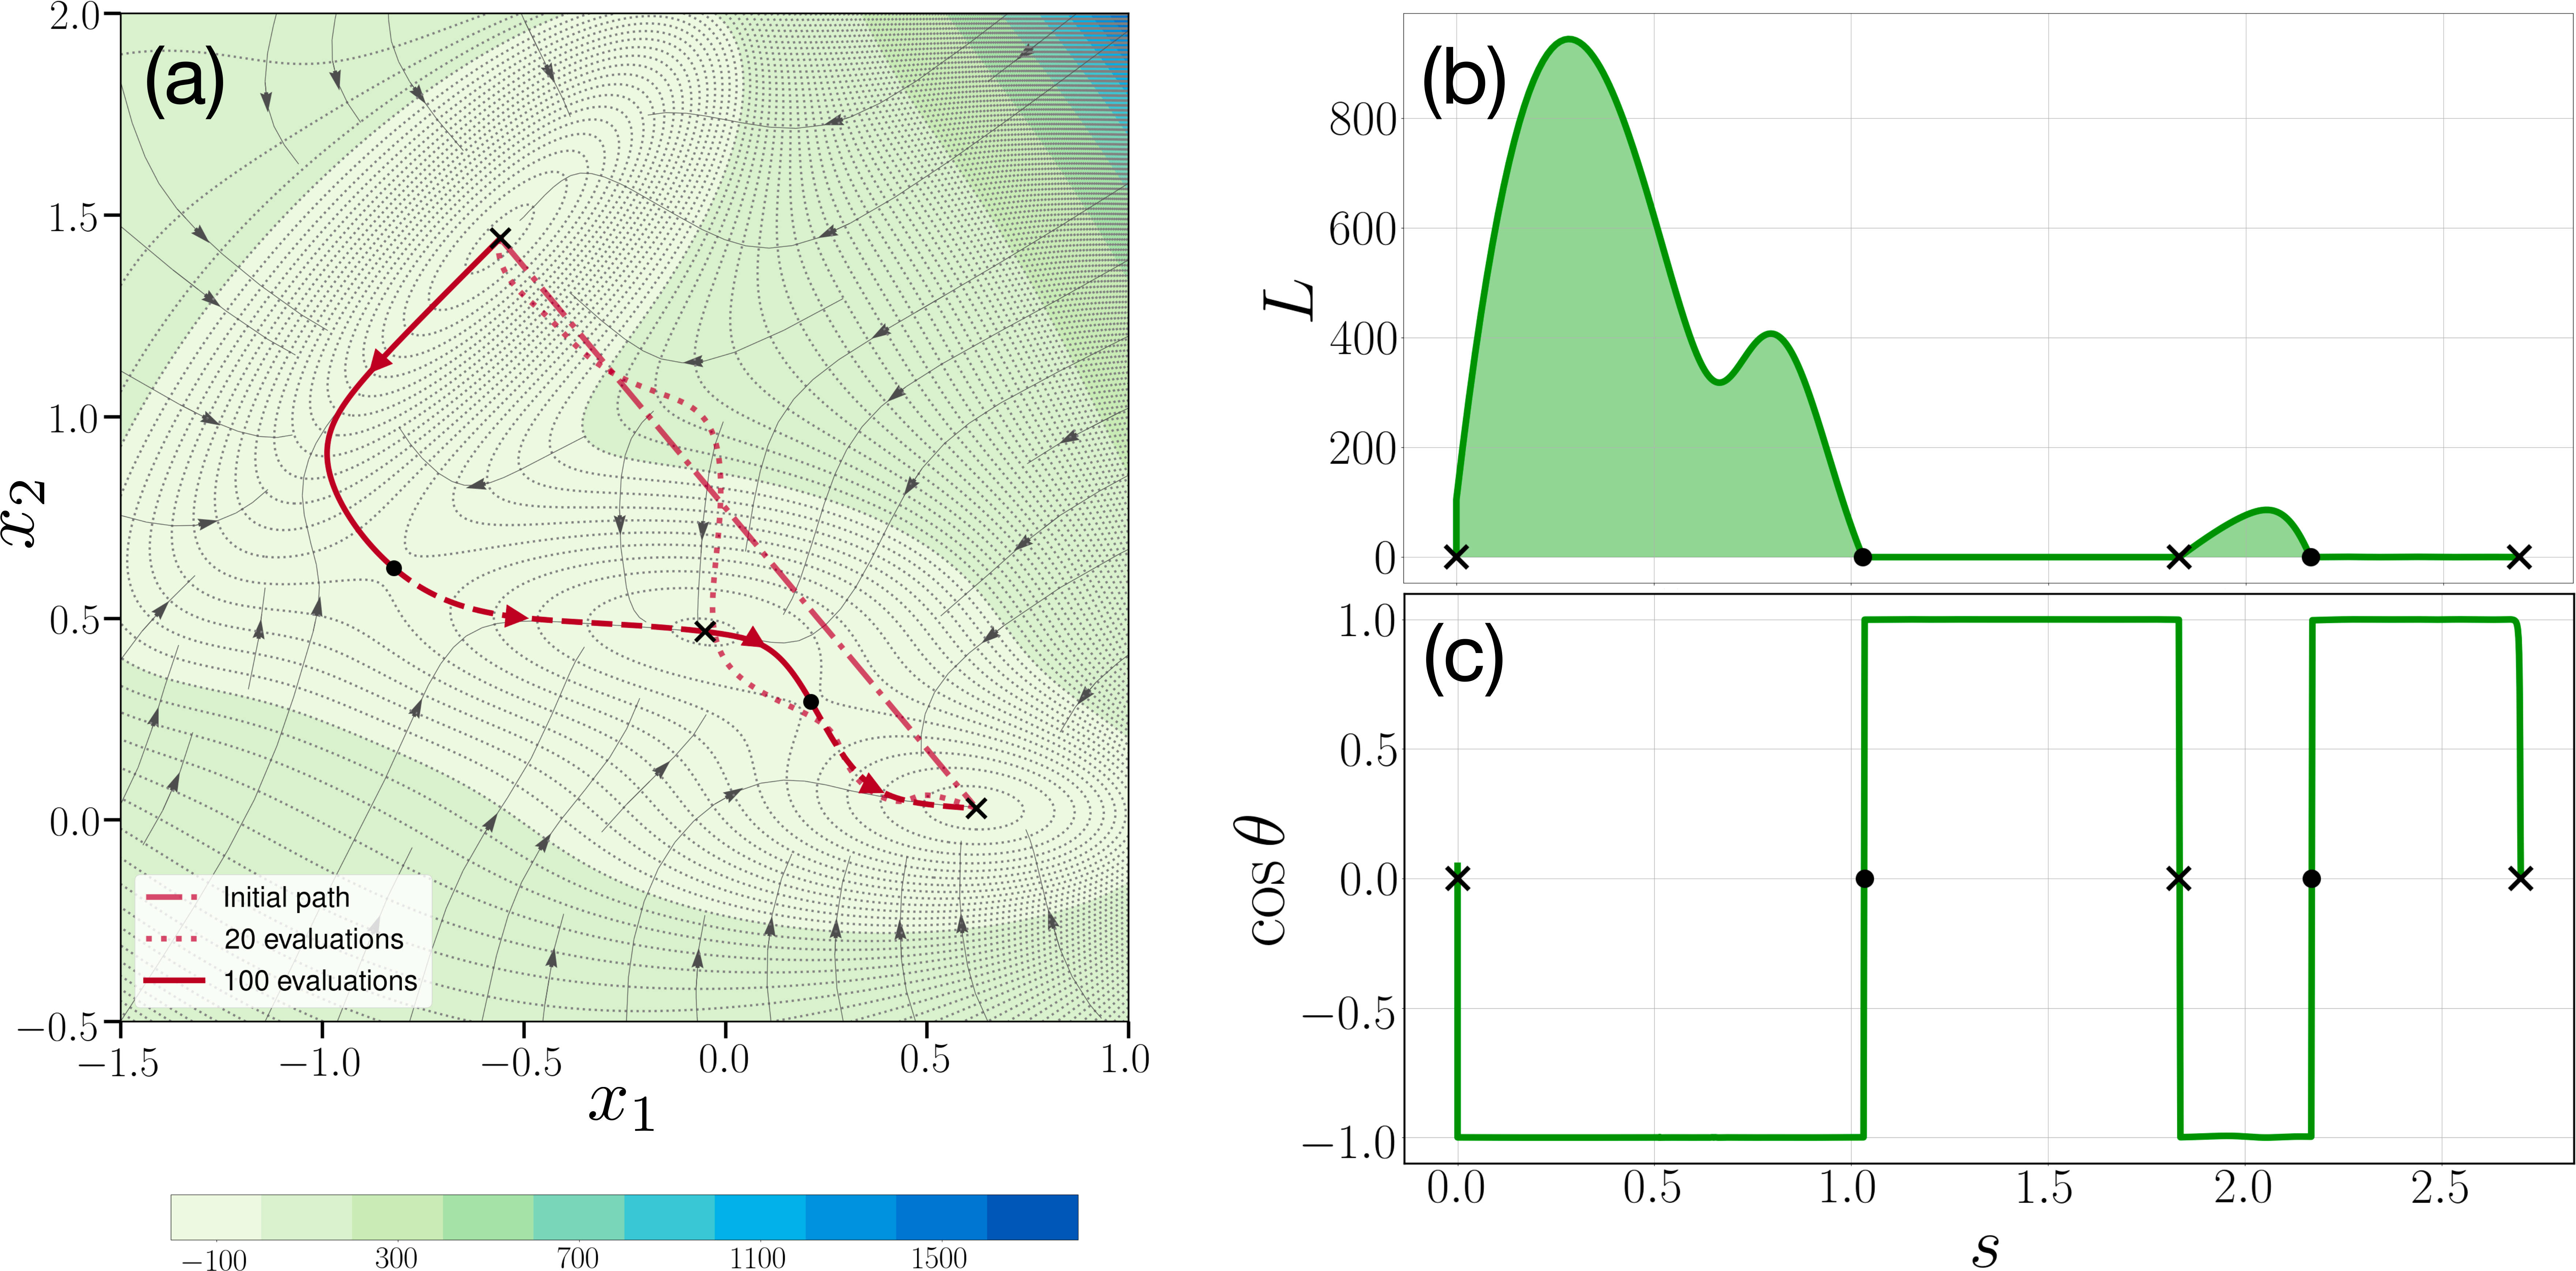
\includegraphics[width=0.94\linewidth]{figs_part1/pyritz/fig1.jpeg}
\par\end{centering}
\caption{Ritz method for overdamped motion in the Müller-Brown potential, which
has three minima (crosses) and two saddle points (dots). The initial
path is the straight line connecting two minima and the instanton
is the solid line, with broken segments showing motion along the force.
The instanton automatically locates and passes through both saddles.
A typical path before convergence to the minimum is shown as a dotted
line. (b) The value of the Lagrangian as a function of Euclidean arc-length
of the instanton. The action vanishes to machine precision on segments
of the path where motion is along the force. (c) The cosine of the
angle $\theta$ between the tangent and the force is always $\pm1$,
i.e. the instanton is a minimum energy path. The instanton is represented
by a polynomial of degree $n=10$. }

\label{fig:muller-brown-instanton}
\end{figure*}


\subsection{Brownian dynamics in a complex potential}

Our first example considers the overdamped Brownian motion in a two-dimensional
potential with a constant friction. The usual equations of Brownian
dynamics can be recast into Itô form,

\begin{align*}
dX_{1} & =-\mu\partial_{1}Udt+\sqrt{2\mu\varepsilon}\,dW_{1}\\
dX_{2} & =-\mu\partial_{2}Udt+\sqrt{2\mu\varepsilon}\,dW_{2},
\end{align*}
where $\mu$ is the mobility and $\varepsilon=k_{B}T$ is the temperature.
The Freidlin-Wentzell action for a smooth path with two-dimensional
coordinate $x=(x_{1},x_{2})$ is
\[
S[x]=\frac{1}{2}\int_{0}^{T}\frac{1}{2\mu}|\dot{x}+\mu\nabla U|^{2}dt
\]
where $\nabla U=(\partial_{1}U,\partial_{2}U)$. The minimum of the
zero-energy action, 

\[
S_{0}[x]=\int_{-1}^{1}|\nabla U(x)||x'|du+\left[U(x)\right]_{-1}^{1},
\]
provides the most probable shape and the stationary quasipotential.
\textcolor{black}{The second term does not affect the minimisation
and can be discarded. The resulting reduced action}

\textcolor{black}{
\begin{equation}
\tilde{S}[x]=\int_{-1}^{1}|\nabla U||x'|du\label{eq:fermat}
\end{equation}
is of the same form as Fermat's principle for optical rays, where
$|\nabla U(x)|$ plays the role of the refractive index and $|x'|du=ds$
is the arc-length of the ray. In geometric optics, Fermat's principle
is equivalent to Huygen's principle and its ``wavelet equation''}

\textcolor{black}{
\begin{equation}
\partial_{i}U=|\nabla U|\frac{dx_{i}}{ds}.\label{eq:huygen}
\end{equation}
}This can be easily verified by differentiatiating it with respect
to arc-length, to obtain the eikonal equation

\textcolor{black}{
\[
\partial_{i}|\nabla U|=\frac{d}{ds}\left[|\nabla U|\frac{dx_{i}}{ds}\right],
\]
which is identical to the Euler-Lagrange equation of the zero-energy
action. The wavelet equation implies that the tangent $t=dx/ds$ to
the path is parallel to the gradient of the potential, or equivalently,
that rays are normal to contours of the potential. This is the well-known
condition for a minimum energy path and was first derived variationally
from the scalar work functional by Olender and Elber \citep{olender1997yet}.
It provides a stringent test of the fidelity of the paths }obtained
by minimisation. 
\begin{figure*}
\begin{centering}
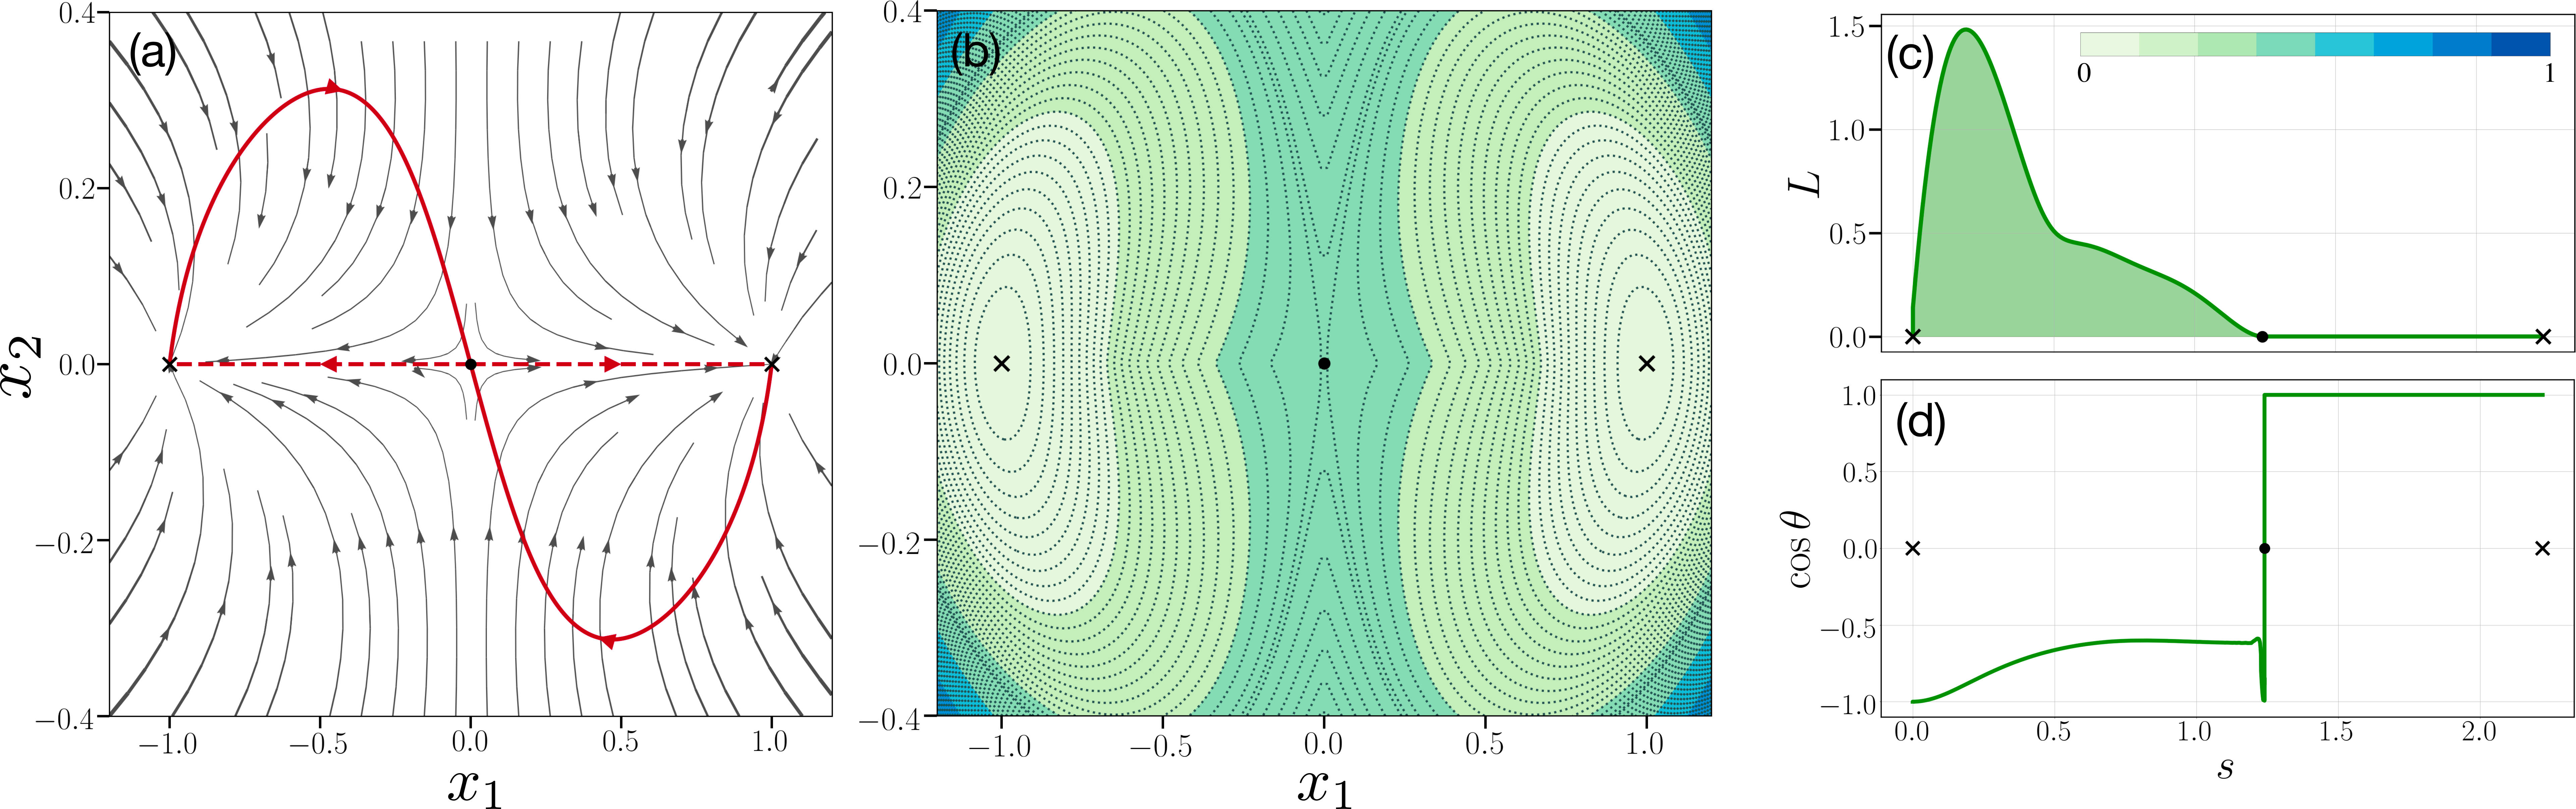
\includegraphics[width=0.99\textwidth]{figs_part1/pyritz/fig2.jpeg}
\par\end{centering}
\caption{Ritz method for overdamped motion in a circulatory (i.e. non-gradient)
force field. The instanton is in red with solid (dashed) segments
showing motion against (along) the force field. The instanton is reflected
about the horizontal axis for motion starting on the right, showing
the inequivalence of fluctuational and relaxational paths for non-gradient
dynamics. (b) The quasipotential, computed using Eq.~\ref{eq:aggregated quasi-potential},
with a caustic at the unstable fixed point. (c) The value of the Lagrangian
as a function of the Euclidean arc-length of the instanton. As in
the potential case, the action vanishes to machine precision on segments
where motion is along the force. (d) The cosine of the angle $\theta$
between the tangent and the force is, unlike in the potential case,
not always $\pm1$. The instanton is represented by a polynomial of
degree $n=8.$ }

\label{fig:maier-stein-quasipotentials}
\end{figure*}

Following \citep{olender1997yet}, we choose the Müller-Brown potential
of \citep{muller1979location} as an example of a complex energy landscape.
The potential and its stationary points are shown in Fig. \ref{fig:muller-brown-instanton}.
The three minima are marked by crosses and two saddle points by dots.
The instanton is computed by requiring the path to start at the minimum
on the top left and terminate at the minimum on the bottom right.
The initial straight line shape, an intermediate shape and the converged
instanton are shown in panel (a). The minimisation automatically locates
the two saddle points and makes the the instanton pass through them.
The action cost along the path is shown in panel (b), where the vanishing
of the action on segments of the path along the force is clearly seen.
The cosine of the angle between the tangent and force is shown in
panel (c) and the condition for a minimum energy path is clearly fulfilled.
We emphasise that the condition is not imposed separately but is satisfied
automatically at the minimum. The Ritz method provides an alternative
to chain-of-states methods for finding minimum energy paths. It does
not need the Hessian of the potential, which makes it suitable for
problems where such evaluations are expensive. Unlike \citep{heymann2008geometric},
our parametrisation has no unit-speed constraint and the minimisation,
accordingly, is unconstrained. The method applies without change to
dynamics with configuration-dependent friction. 


\subsection{Brownian dynamics in a circulatory field}

For our second example we consider, in contrast to the first, Brownian motion
in a force field that cannot be derived from a potential and, as such,
necessarily has a non-vanishing curl. Choosing the force field of
Maier and Stein \citep{maier1996scaling} gives

\[
\begin{aligned}dX_{1}= & (X_{1}-X_{1}^{3}-\beta X_{1}X_{2}^{2})dt+\sqrt{\epsilon}dW_{1}\\
dX_{2}= & -(1+X_{1}^{2})X_{2}dt+\sqrt{\epsilon}dW_{2}
\end{aligned}
\]
for the overdamped motion of the two-dimensional coordinate $X=(X_{1},X_{2})$,
where $\beta$ is a parameter. The force field $f(x_{1},x_{2})=(x_{1}-x_{1}^{3}-\beta x_{1}x_{2}^{2},-(1+x_{1}^{2})x_{2})$
is smooth, and $f_{1}$ is odd in $x_{1}$ and even in $x_{2}$, while
for $f_{2}$ the converse holds. There are two stable fixed points
at $x_{a}=(-1,0)$ and $x_{b}=(1,0)$, and a saddle point at $x_{s}=(0,0)$.
The force field admits a potential only for $\beta=1$, when it can
be written as $f=-\nabla U$, with $U(x_{1},x_{2})=-\frac{1}{2}x_{1}^{2}+\frac{1}{4}x_{1}^{4}+\frac{1}{2}(1+x_{1}^{2})x_{2}^{2}$.
The force field is shown in the first panel of Fig. \ref{fig:maier-stein-quasipotentials}
for $\beta=10$ together with the instanton moving from $x_{a}$ to
$x_{b}$. As before, solid (dashed) segments represent motion against
(along) the vector field. The instanton moving from $x_{b}$ to $x_{a}$
is obtained by reflection about the $x_{1}$-axis showing that that
fluctuational and relaxational paths are not identical in a non-gradient
field. 

The middle panels shows the stationary quasipotential $V_{\infty}^{\mathcal{A}_{i}}(x)$
with respect to the attractors at $(-1,0)$ and $(1,0)$ respectively.
The quasipotential is sampled on a $128\times128$ grid by computing
instantons between a point on the grid and the relevant attractor.
The contours of the quasipotential and its heatmap are obtained from
these discrete samples. To the best of our knowledge, all prior estimations
of the quasipotential for this problem (and more generally, for circulatory
forces) have required numerical solutions of the Hamilton-Jacobi equation.
Our method of direct sampling provides an alternative to this route
of computing the quasipotential. The right panel shows the Lagrangian
as a function of arc-length along the instanton. As in the previous
example, the Lagrangian vanishes along segments of the path where
motion is along the force. For motion against the force, the tangent
to the path is no longer parallel to the force, as shown by the variation
of the cosine of the angle $\theta$ between the tangent and the force.
We note that our method is agnostic to the existence, or not, of a
potential for the drift and treats both these cases on equal footing.


\subsection{Multistability in a genetic switch}

We continue with the dynamics of a two-dimensional coordinate $x=(x^{1},x^{2})$
in a non-gradient field, but now of non-mechanical origin and non-polynomial
form,

\begin{equation}
\begin{aligned}dx^{1} & =\left(\frac{a_{1}}{1+\left(\frac{x^{2}}{K_{2}}\right)^{n}}-\frac{x^{1}}{\tau}\right)dt+\sqrt{\epsilon}dW^{1}\\
dx^{2} & =\left(\frac{a_{2}}{1+\left(\frac{x^{1}}{K_{1}}\right)^{m}}-\frac{x^{2}}{\tau}\right)dt+\sqrt{\epsilon}dW^{2},
\end{aligned}
\label{eq:genetic-switch}
\end{equation}
where $a_{1},$ $a_{2}$, $\tau$, $n$, $m$, $K_{1}$ and $K_{2}$
are constants. This model is due to Roma \emph{et al} \citep{roma2005optimal}
and describes a multistable genetic network. In the region of configuration
space we consider, the vector field has two fixed points one of which
is stable and the other a saddle. The top panel of Fig. \ref{fig:genetic-switch-quasipotential}
shows the instantons moving between these fixed points. Unlike in
the previous examples, here the instantons move either entire with
(solid line) or entirely against (dashed line) the flow. The bottom
panel shows the quasipotential with respect to the stable fixed point.
The procedure to evaluate and plot it is as described above. The quasipotential
provides a quantification of the dispersion of the coordinate about
the stable fixed point and a measure of the non-equilibrium ``temperature''
of this non-mechanical system. 

\begin{figure*} 
    \centering
     
    \begin{subfigure}[b]{0.4\textwidth}  
        \centering 
        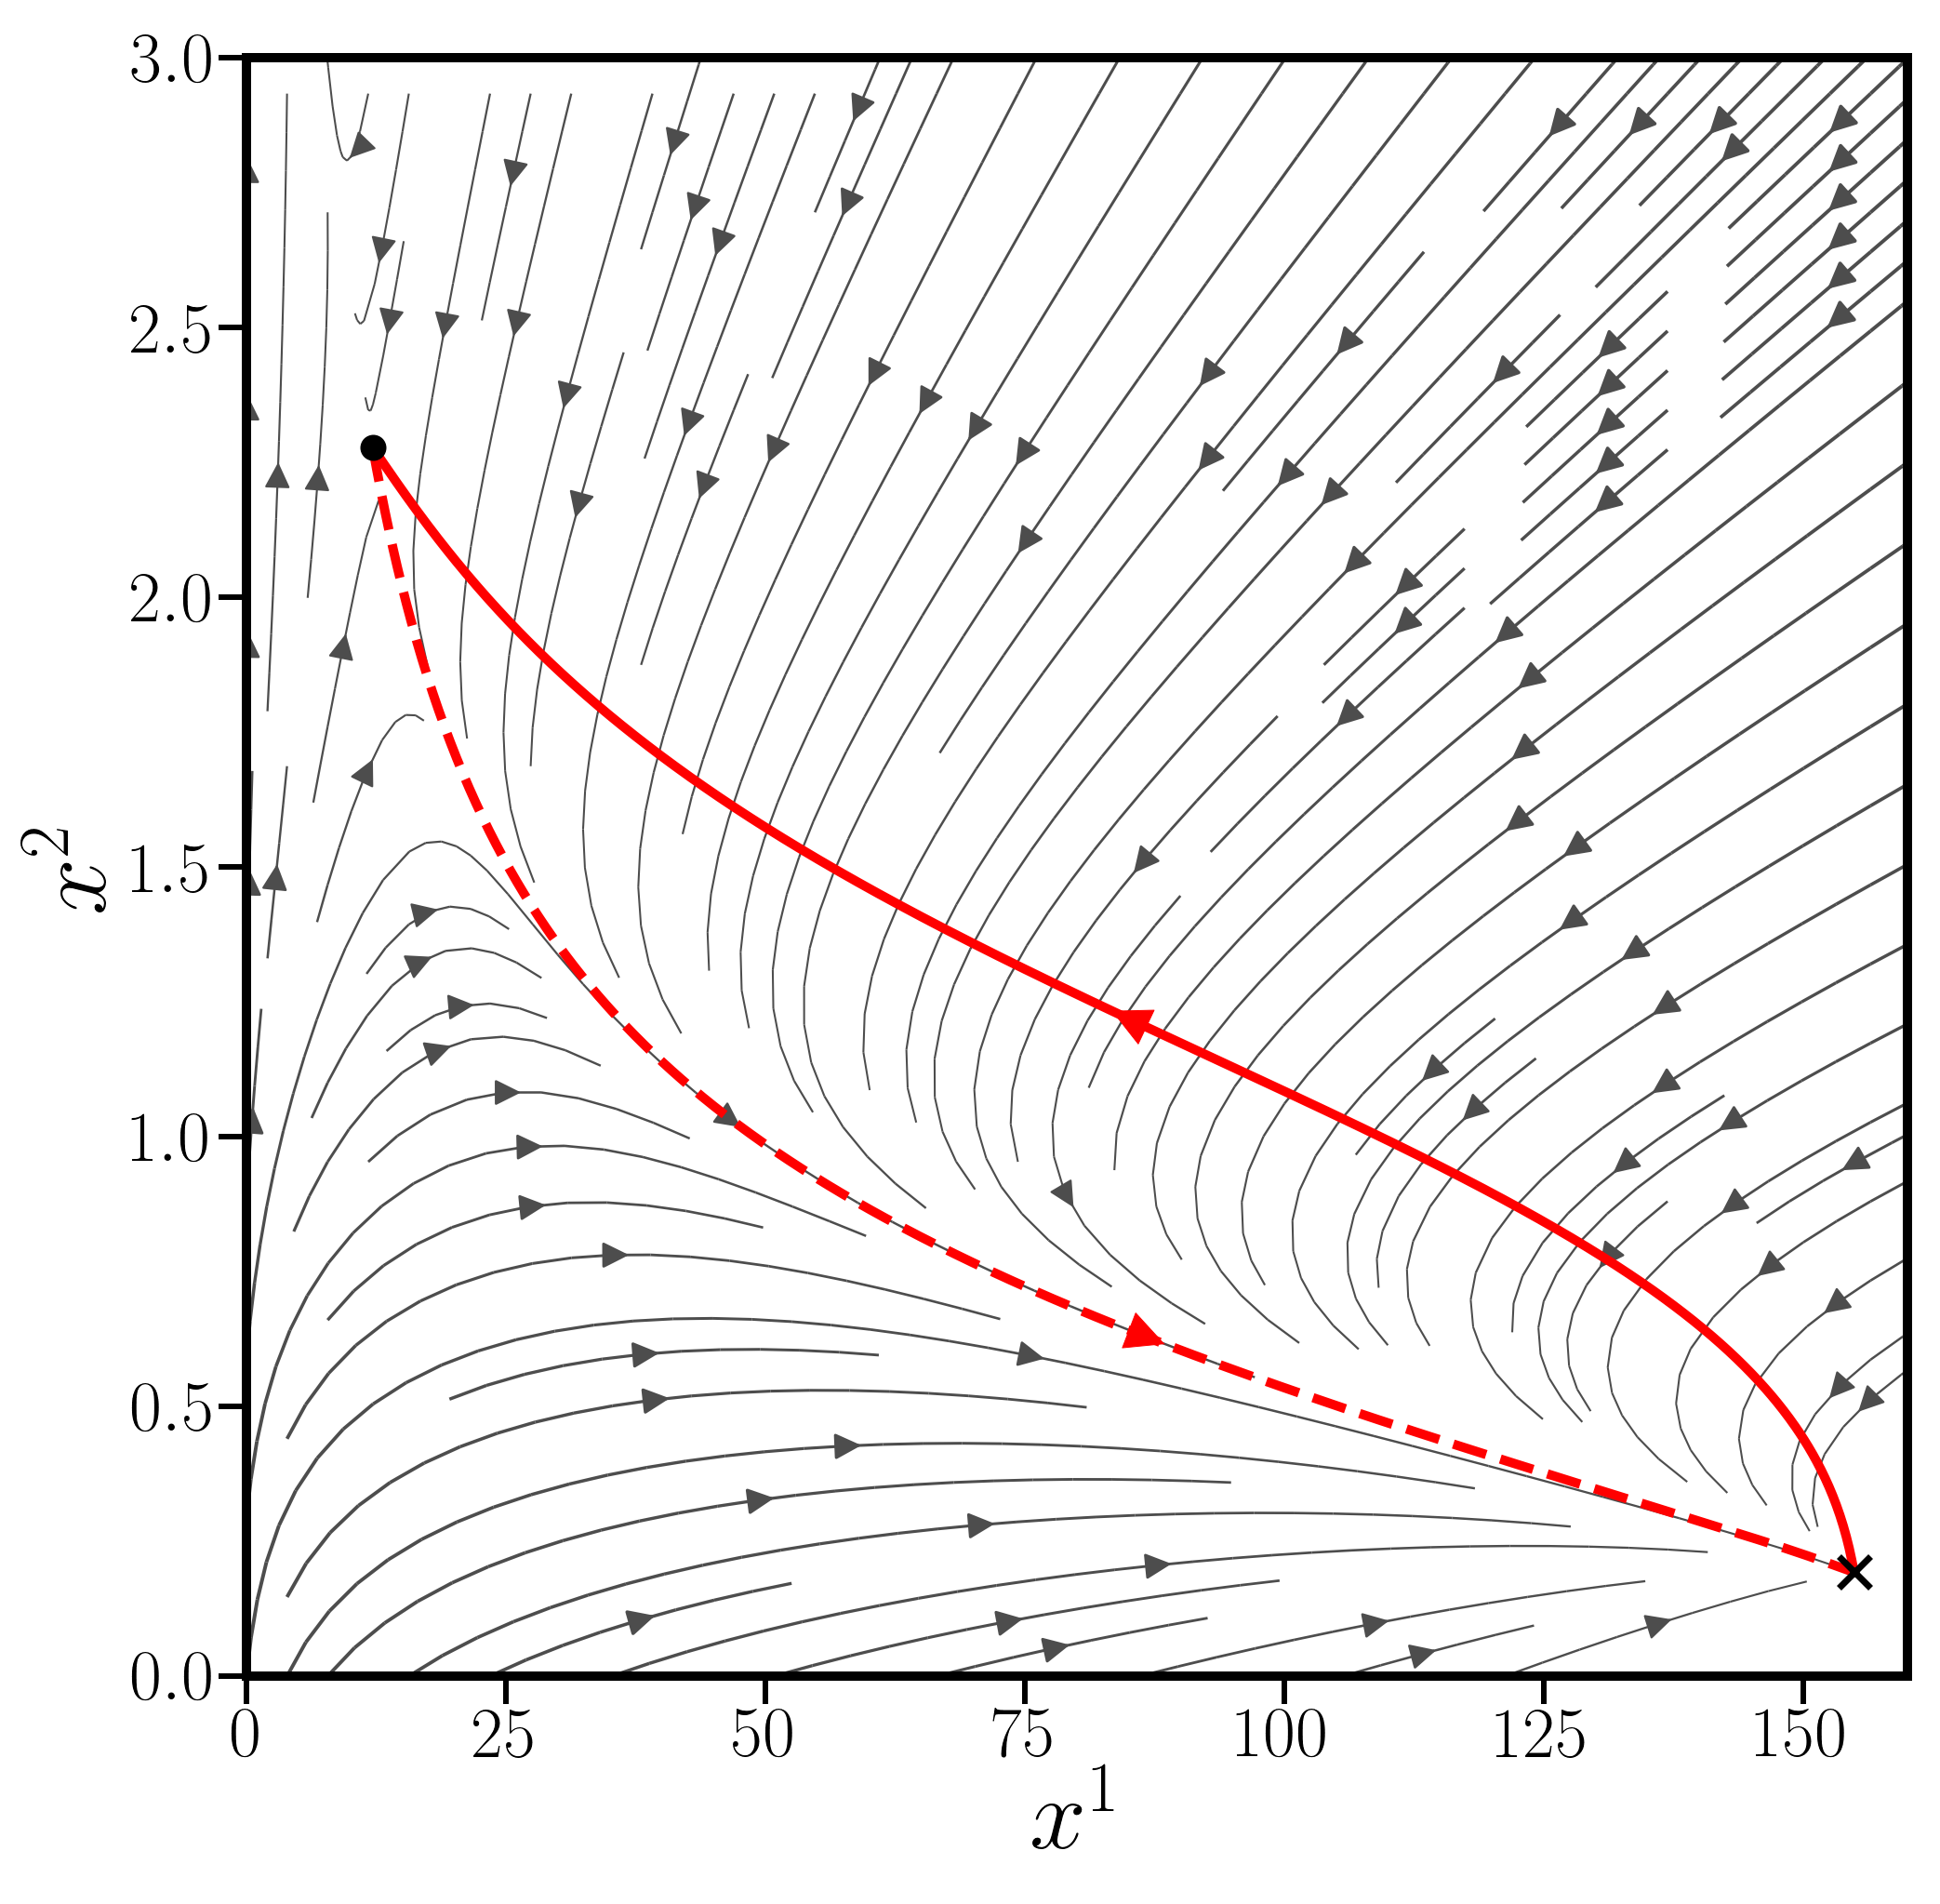
\includegraphics[width=\textwidth]{figs_part1/pyritz/genetic_switch_instanton.png}
        \caption[]%
        {}    
        \label{fig:straight cosserat rod}
    \end{subfigure}
    \hspace{0.4cm}
    \begin{subfigure}[b]{0.4\textwidth}
        \centering
        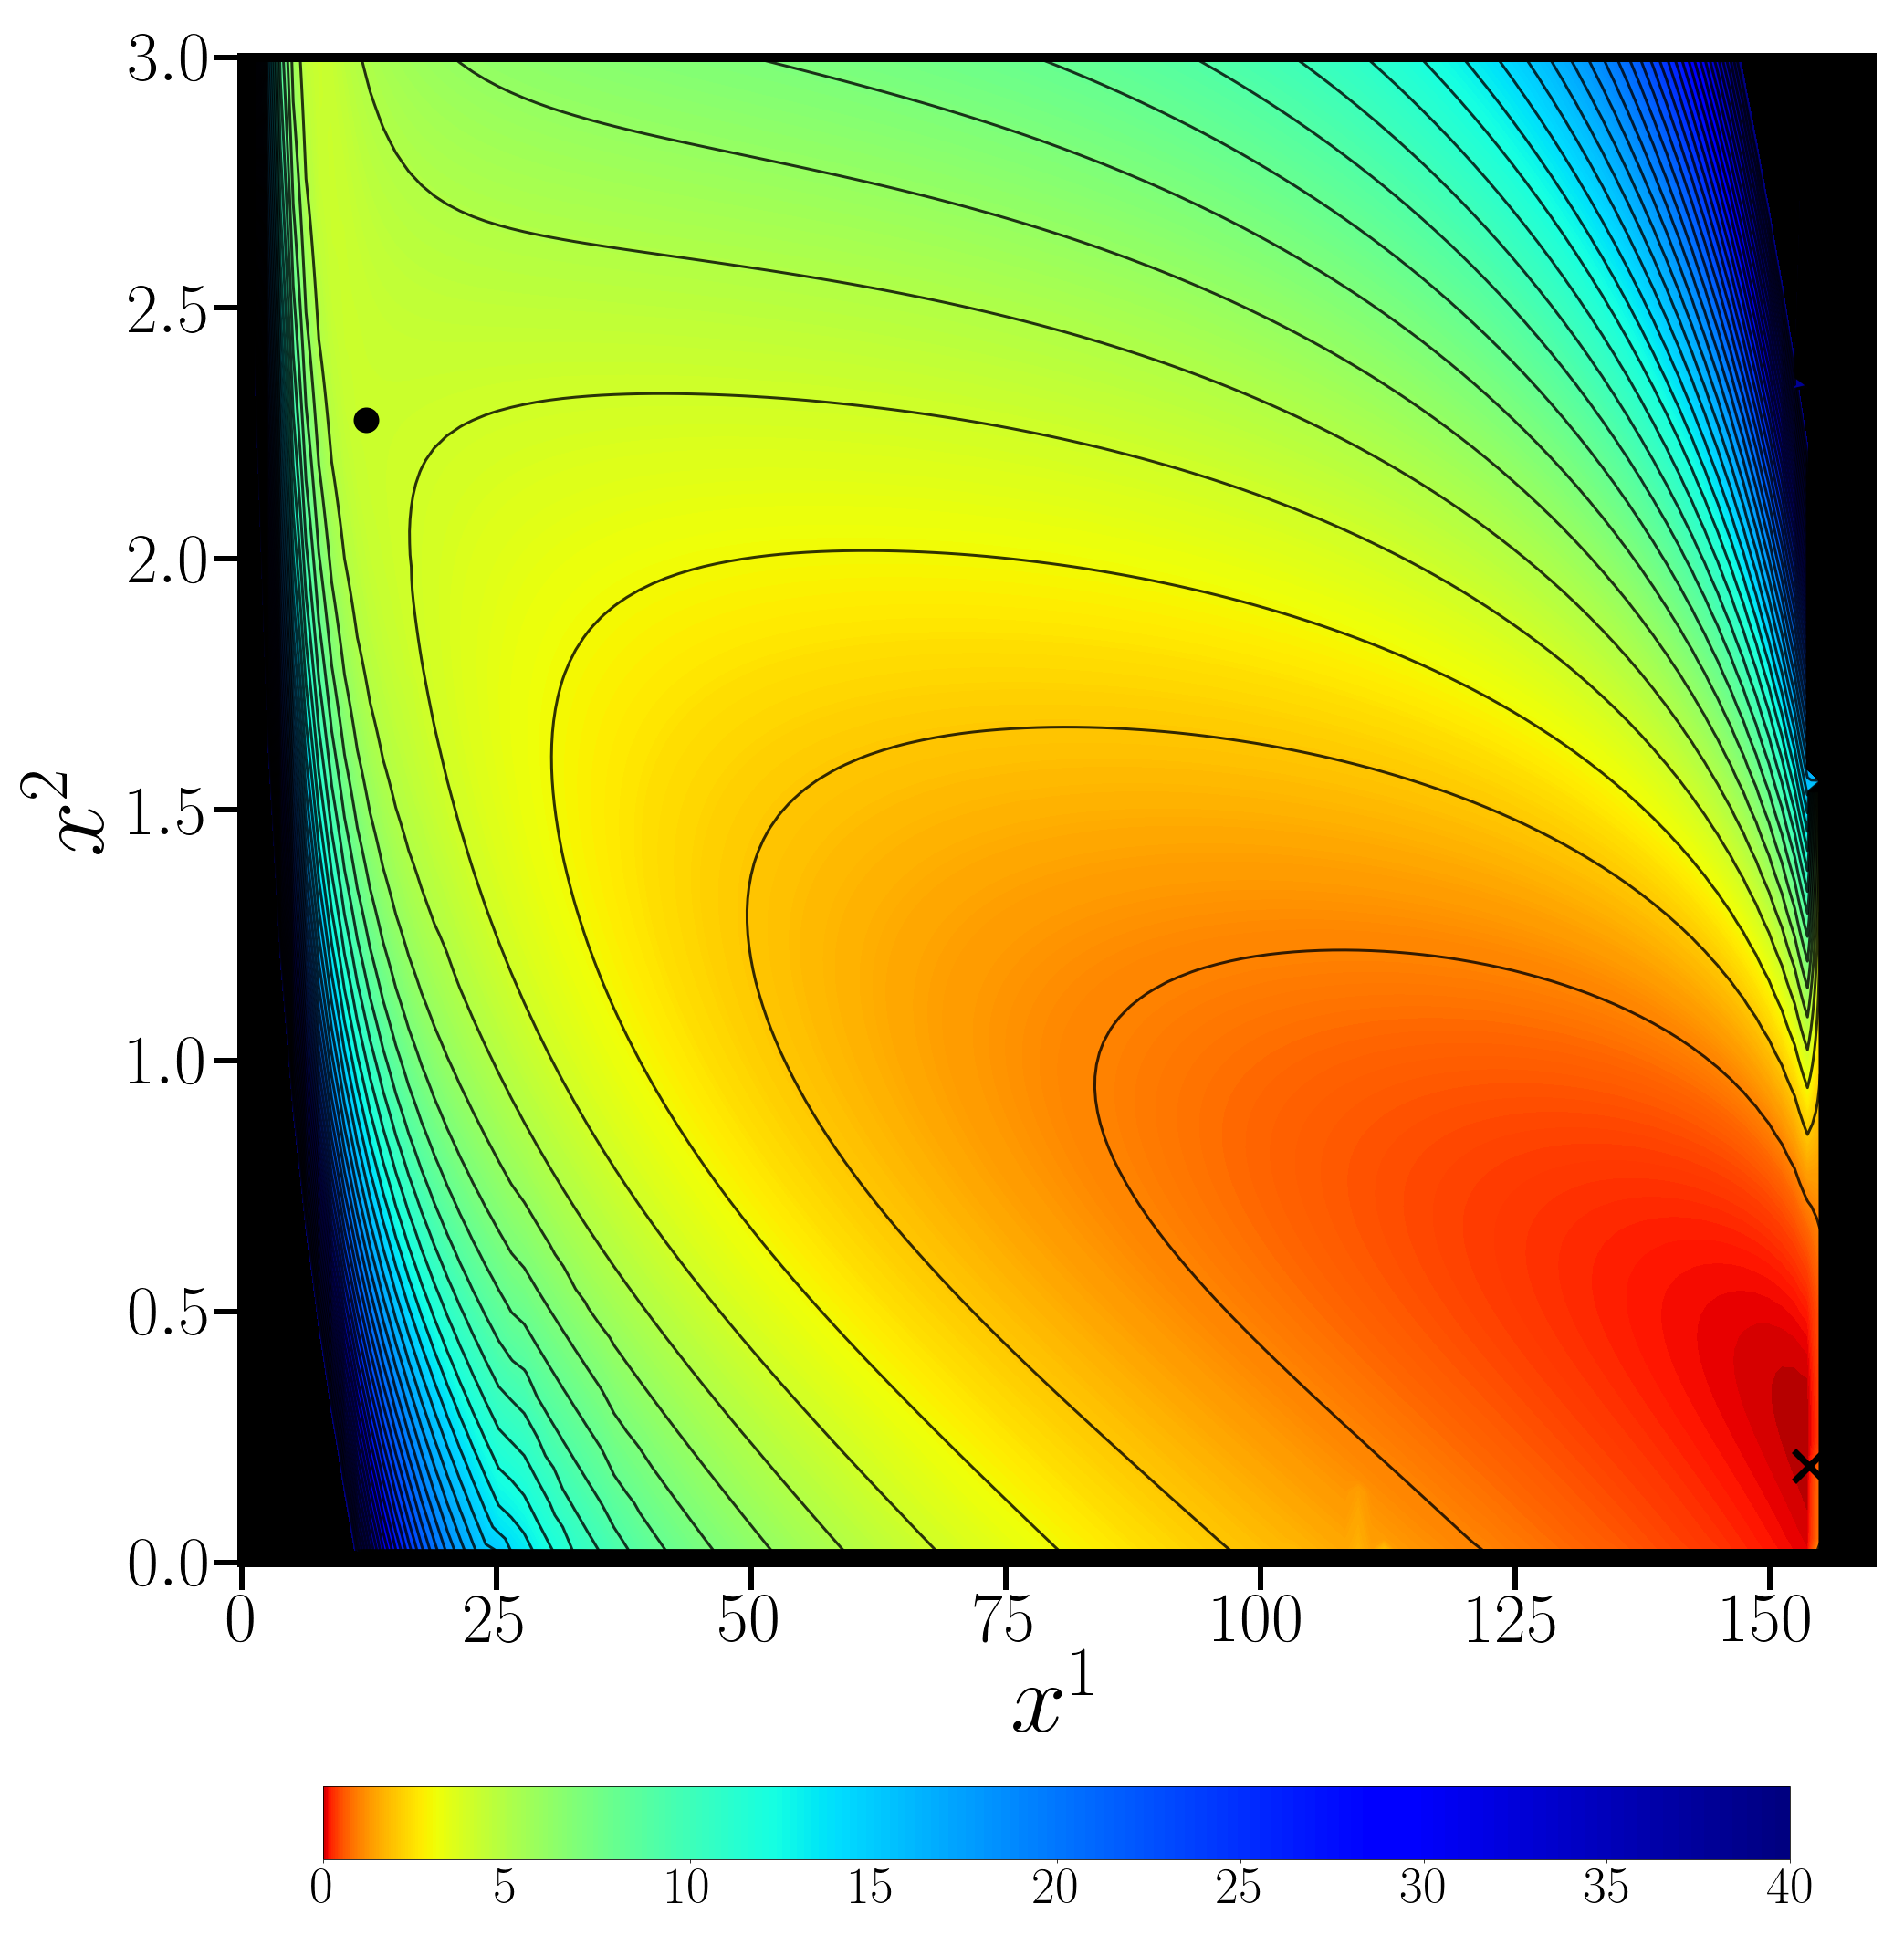
\includegraphics[width=\textwidth]{figs_part1/pyritz/genetic_switch_quasipotential_from_xb_to_xa.png}
        \caption[Extending Cosserat rod]%
        {}    
        \label{fig:extending cosserat rod}
    \end{subfigure}    
    \caption[ ]
    {\small Instantons for the genetic switch. (a) shows the instantons
in red with solid (dashed) lines representing motion against (along)
the vector field. (b) shows the quasipotential with respect
to the stable fixed point (cross). Parameter values are $a_{1}=156$, $a_{2}=30$,
$\tau=1$, $n=3$, $m=1$ and $K_{1}=K_{2}=1$. A polynomial of degree $n=10$ was used to parametrise the path.} 
    \label{fig:genetic-switch-quasipotential}
\end{figure*} 



\subsection{Transitions between limit cycles}

To demonstrate that our method is not limited to fixed points, we
constructed a simple but non-trivial system:

\begin{equation}
\begin{aligned}dr & =(1+\cos^{2}\theta)f(r)dt+dW^{r}\\
d\theta & =r(1+\sin^{2}\theta)dt+dW^{\theta}
\end{aligned}
\label{eq:limit-cycle system}
\end{equation}
where $f(r)=-\frac{1}{4}r(r-s_{1})(r-s_{2})(r-s_{3})$, and $s^{(i)}=[1,3,5]$.
We have an unstable fixed point at $r=0$, stable limit cycles at
$r=s_{1}$ and $r=s_{3}$, and an unstable limit cycle at $r=s_{2}$.
The trigonometric factors in the drift breaks the circular symmetry
of the system, but preserves the concentric circular limit cycles.
We consider instantons moving from the inner stable limit cycle $r=s_{1}$
to the outer limit cycle $r=s_{3}$. Let $\Gamma_{i}=\{(r,\theta)\,|\,r=s_{i}\}$
for $i=1,2,3$, be the set of points comprising the three limit cycles.
For a given path $x(t)$, let $x_{i}\in\Gamma_{i}$ be the points
along the path located along the respective limit cycles. Since $a_{r}(x_{i})=0$
and $a_{\theta}(x)$ is positive definite, the system can move to
any point within a limit cycle without incurring any action cost.
Therefore the starting, intermediate and end points $x_{1}$, $x_{2}$
and $x_{3}$ should be varied freely within their respective limit
cycles during the minimisation. We can split the instanton $x^{*}(t)$
into an ``uphill'' path $x_{\uparrow}^{*}(t)$, moving between $\Gamma_{1}$
and $\Gamma_{2}$, and a ``downhill'' path $x_{\downarrow}^{*}(t)$,
moving between $\Gamma_{2}$ and $\Gamma_{3}$. The downhill path
follows deterministic relaxational dynamics, and does not contribute
to the action, and therefore the only non-trivial part of the problem
is the uphill path $x_{\uparrow}^{*}(t)$. One issue with limit cycle
problems is that instantons in general have infinite arc-lengths.
In the case of the relaxational path $x_{\downarrow}^{*}(t)$, this
can be verified to be the case using an ODE solver. The system will
not only relax to the attractor in infinite time, but the system will
also undergo an infinite number of cycles before reaching the stable
limit cycle $\Gamma_{3}$. We would expect similar behaviour for diffusive
paths leaving stable limit cycles. Paths of infinite Euclidean arc-length
are not possible to parametrise exactly in the Chebyshev basis, so
only an approximate finite-length instanton can be found, as shown
in Fig. \ref{fig:concentric}. As we increased the arc-length the action of the candidate instanton converged to a value of $S\approx3.65053$.
\begin{figure}[t]
\begin{centering}
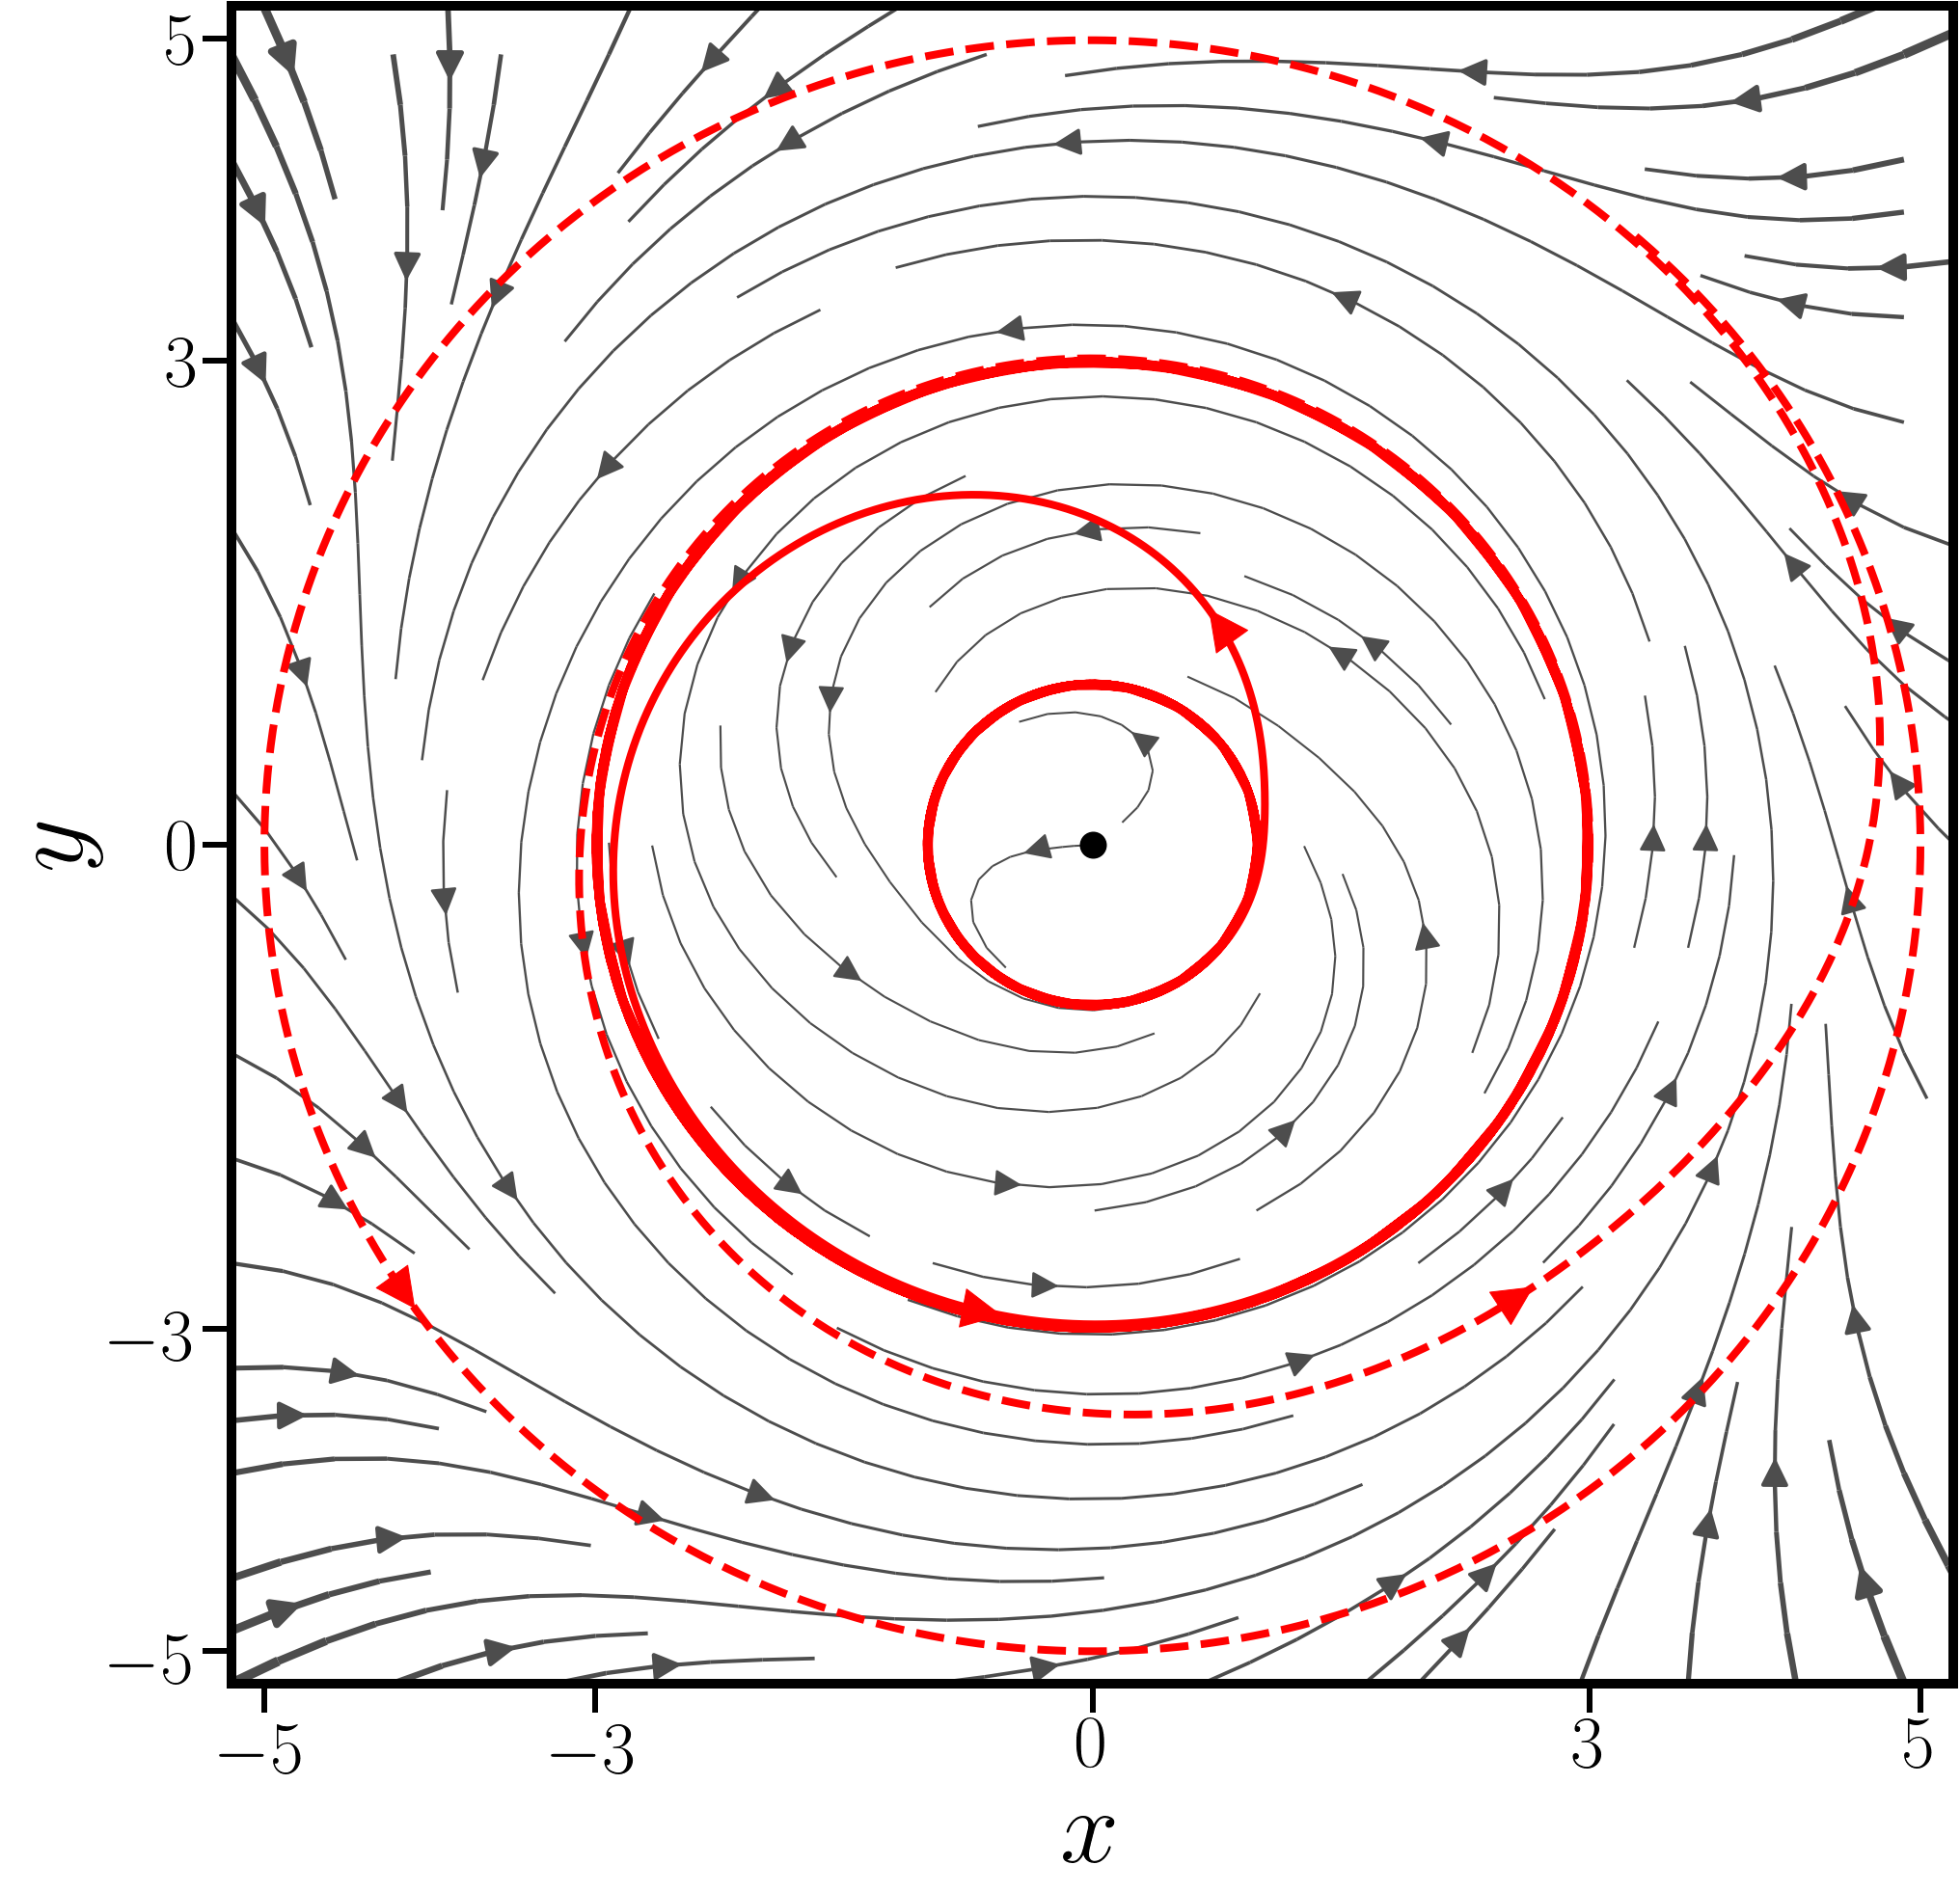
\includegraphics[width=0.7\columnwidth]{figs_part1/pyritz/concentric_limit_cycle_instanton.png}
\par\end{centering}
\caption{An approximate instanton of the concentric limit cycle system with $S\approx3.65053$.
The instanton moves from the inner stable limit cycle at $r=1$ to the unstable limit cycle at $r=3$, and then moves hetero-clinically along the drift to the outer stable limit cycle at $r=4$.}
\label{fig:concentric}
\end{figure}

\subsection{Egger model of weather}

\begin{figure*}
\begin{centering}
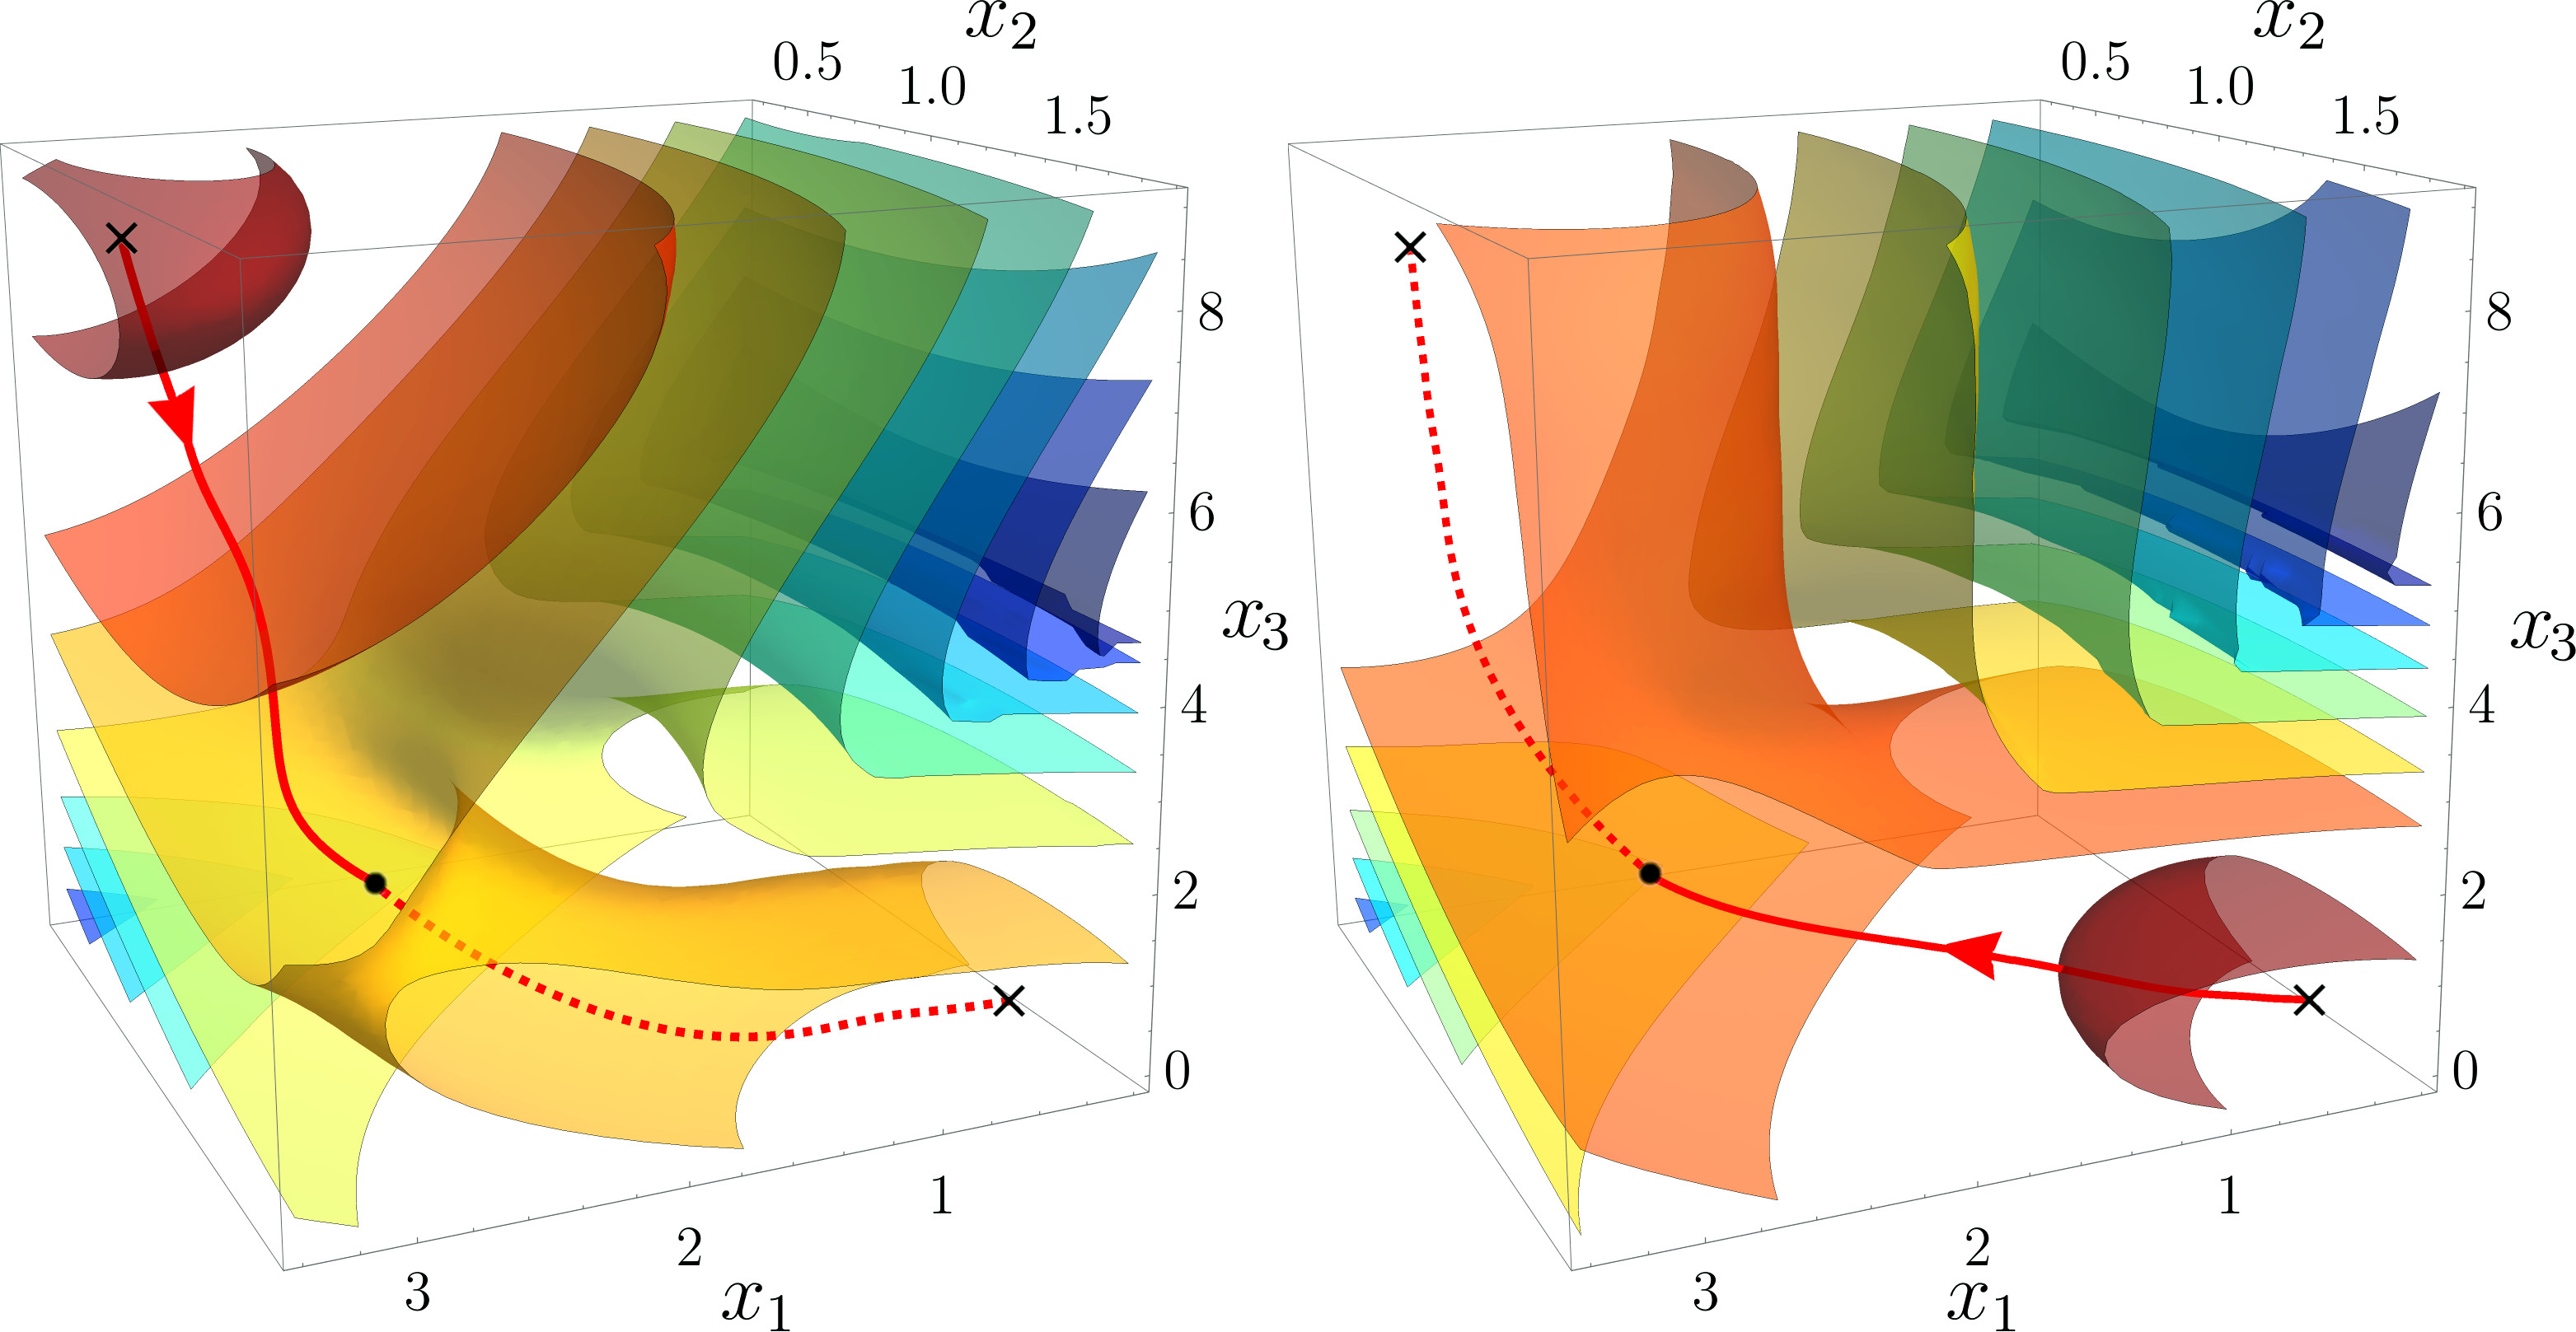
\includegraphics[width=0.9\textwidth]{figs_part1/pyritz/fig3.jpeg}
\par\end{centering}
\caption{Instantons and quasi-potentials of the Egger model. The instantons
are shown in red with solid (dashed) lines representing motion against
(along) the vector field. The left and right panels are forward and
reverse instantons. Isosurfaces of the quasipotential with respect
to each attractor is shown in the respective panels. Isovalues increase
from light red to blue in the range $\left\{ 1,7,11,16,21,26,31,36\right\} $.
Parameter values are $k=2$, $\beta=1.25$, $\gamma=2$, $U_{0}=10.5$
and $H=12$. The instanton is represented by a polynomial of degree
$n=10.$}
\centering{}\label{fig:eggers}
\end{figure*}

Our final example is a reduced model of the weather for a a three-dimensional
coordinate $X=(X_{1},X_{2},X_{3})$ that has a circulatory drift,
\begin{alignat}{1}
dX_{1}= & \left[kX_{2}\left(X_{3}-\frac{\beta}{k^{2}}\right)-\gamma X_{1}\right]dt+\sqrt{\epsilon}dW_{1}\nonumber \\
dX_{2}= & \left[kX_{1}\left(\frac{\beta}{k^{2}}-X_{3}\right)-\gamma X_{2}+\frac{HX_{3}}{k}\right]dt+\sqrt{\epsilon}dW_{2}\nonumber \\
dX_{3}= & \left[-\tfrac{1}{2}HkX_{2}-\gamma(X_{3}-U_{0})\right]dt+\sqrt{\epsilon}dW_{3}\label{eq:egger}
\end{alignat}
where $k$, $\beta$, $\gamma$, $U_{0}$ and $H$ are constants.
This model is due to Egger \citep{egger1981stochastically}. It is
not particularly illuminating to visualise the three-dimensional vector
field describing this dynamics but we note that it has two stable
fixed points, marked by crosses in Fig. \ref{fig:eggers}, and a saddle
fixed point marked by a dot. The instanton moving between these points
is shown as before in the left and right panels of the figure. Also
shown are isosurfaces of the quasipotential with respect to the stable
fixed points, with isovalues increasing from red to blue. To the best
of our knowledge, this is the first computation of the quasipotential
for this model. We provide this example primarily to demonstrate the
feasibility of sampling quasipotentials in dimensions greater than
two with our method. 

\setlength{\tabcolsep}{2.5pt}

\begin{table}
\begin{centering}

\begin{tabular}{|c|c|c|c|c|c|}
\hline 
Model & $S_{1}-S_{2}$ & $S_{3}-S_{4}$ & $S_{7}-S_{8}$ & $S_{15}-S_{16}$ & $S_{31}-S_{32}$\tabularnewline
\hline 
\hline 
M-B & $2$ & $3\times10^{-4}$ & $1\times10^{-7}$ & $5\times10^{-14}$ & $1\times10^{-13}$\tabularnewline
\hline 
M-S & $2\times10^{-3}$ & $3\times10^{-7}$ & $2\times10^{-12}$ & $1\times10^{-16}$ & $5\times10^{-16}$\tabularnewline
\hline 
Egger & $8\times10^{-3}$ & $1\times10^{-3}$ & $6\times10^{-7}$ & $4\times10^{-9}$ & $8\times10^{-13}$\tabularnewline
\hline 
\end{tabular}%

\vspace{0.2cm}

\begin{tabular}{|c|c|c|c|c|c|}
\hline 
Model & $S_{2}-S_{50}$ & $S_{4}-S_{50}$ & $S_{8}-S_{50}$ & $S_{16}-S_{50}$ & $S_{32}-S_{50}$\tabularnewline
\hline 
\hline 
M-B & $4\times10^{-2}$ & $4\times10^{-5}$ & $8\times10^{-8}$ & $1\times10^{-12}$ & $3\times10^{-13}$\tabularnewline
\hline 
M-S & $2\times10^{-4}$ & $7\times10^{-11}$ & $2\times10^{-13}$ & $1\times10^{-16}$ & $2\times10^{-16}$\tabularnewline
\hline 
Egger & $5\times10^{-3}$ & $1\times10^{-4}$ & $1\times10^{-6}$ & $1\times10^{-8}$ & $2\times10^{-10}$\tabularnewline
\hline 
\end{tabular}

\par\end{centering}
\caption{Convergence of the action $S_{n}$ for a path of polynomial order
$n$. The abbreviations M-B and M-S refer to Brownian dynamics in
the Müller-Brown potential and the Maier-Stein force field respectively.
The first table shows the difference $S_{n}-S_{n+1}$ while
the second table shows the difference $S_{n}-S_{50}$. A tenth-order polynomial
typically gives at least six digits of accuracy. \textcolor{red}{\label{tab:Convergence}}}
\end{table}

\section{Numerical convergence}

We briefly recall the convergence properties of the Ritz method, comprising
that of the basis functions, the quadrature, and the optimisation.
The Chebyshev interpolant converges to the most probable
path, assuming that it is Lipschitz continuous, at a rate that increases
with the number of derivatives the path admits and is exponential
for a smooth path. Likewise, the Clenshaw-Curtis quadrature is guaranteed
to converge to the minimum of the action, assuming that the Lagrangian
is Lipschitz continuous. The optimal number of quadrature points for
accuracy to machine precision can be obtained by following the decay
of the Chebyshev coefficients of the Lagrangian and truncating at
that value beyond which the coefficients vanish to machine precision.
The optimisation has lesser theoretical guarantees than the interpolation
and quadrature, as is generally the case with search in high-dimensional
spaces. However, the residual of the Ritz system provides an empirical
measure for how closely the minimum has been located. In all three
examples (and in others not presented here) we have found both gradient-free
and gradient-based optimization to robustly locate the minima, and
gradient-based methods to yield faster convergence. We note that for
equilibrium problems, the gradient-free method does not require the
Hessian of the energy function, which can be of significant computational
advantage. In Table \ref{tab:Convergence} we show the spectral convergence
of the action with increasing polynomial order of the path for each
of our examples. 

\section{Conclusion}

We have presented an efficient and accurate numerical method for computing
most probable transitions paths and quasipotentials of rare diffusive
events. The method directly minimises the Freidlin-Wentzell action
and thus provides a unified approach for transition
paths in both equilibrium and non-equilibrium systems. Our reparametrisation-invariant
form of the action, derived using a Noether symmetry, is well-suited
for numerical work and is a generalisation of the geometric action.
This frees us from the constraints of the commonly used arc-length
path parametrisation and offers the maximum flexibility in choosing
the space of polynomials in which action is minimised. Thus our method
is not limited to the Chebyshev polynomials in $[-1,1]$ used here
but easily admits trigonometric polynomials and, more generally, any
global basis. Numerical quadrature reduces the action to a multivariate
function of coefficients of the path polynomial whose minimum is obtained
by both gradient-free and gradient-based optimisation. This gives,
simultaneously, both the minimum value of the action and the most
probable path. This efficiency of the method allows us to repeatedly
compute minimum action paths between an attractor and a point in its
basin of attraction and, thereby, map out the quasipotential. The
quasipotential in a non-equilibrium steady state has the same significance
as the Gibbs distribution in equilibrium and our method provides a
robust way of obtaining it without the need to numerically solve the
Hamilton-Jacobi partial differential equation. 
\begin{figure}
\begin{center}
\begin{tikzcd}[column sep=small, row sep=small]      
& S[x] \arrow{ddl}[swap]{\delta} \arrow{ddr}{\mathcal{P}} &
\\     &  &
\\[2ex]     
\delta S[x]=0  & & S(\alpha) \hspace{0.5cm}
\end{tikzcd}
\end{center}  
\begin{center}
\vspace{-0.6cm}
\begin{tikzcd} 
\arrow{d}[swap]{\mathcal{P}} &     \arrow{d}{\nabla} 
\\[2ex]     
\text{Discrete E-L} & \text{Ritz system} 
\end{tikzcd} 
\end{center}  

%\begin{center}
%\begin{tikzcd} [column sep=small, row sep=small]
%\delta,\nabla,\pi \rightarrow \text{variation, extremization, %projection}
%\end{tikzcd} 
%\end{center}  

\caption{Inequivalence of the direct and Euler-Lagrange routes to numerical
action minimization. Here, $\delta$ $\rightarrow$ functional variation,
$\mathcal{P}\rightarrow$ finite-dimensional projection, and $\nabla\rightarrow$
function minimisation. On the left branch, the action is first varied
to obtain the Euler-Lagrange equation and then projected onto a finite-dimensional
basis for numerical solution. On the right branch, the action is first
projected onto a finite-dimensional basis and then minimised to obtain
the Ritz system. The finite-dimensional projection of the Euler-Lagrange
equations is, in general, not identical to the Ritz system.}

\centering{}\label{fig:discrete-el-versus-ritz}
\end{figure}

The direct method used here consists of a discretisation of the action
followed by a search for the minimum in the resulting finite-dimensional
space, expressed schematically in Fig. (\ref{fig:discrete-el-versus-ritz}).
In contrast, the majority of methods impose the vanishing variation
of the action and then search for the solution of the Euler-Lagrange
equation in a finite-dimensional space. The resulting discretised
Euler-Lagrange equations is, in general, not identical to the Ritz
system; in other words, these two methods of reducing an infinite-dimensional
problem to a finite-dimensional one are not equivalent. In contrast
to mechanics, where Newton's equations of motion are considered primary
and the action derived, here it is the tube probability and hence
the Freidlin-Wentzell action that is primary and the Euler-Lagrange
equation for the most probable path that is derived. It appears more
natural to us to discretise the primary, rather than the derived,
object directly. Our approach is algorithmically simple and the only
adjustable parameters are the polynomial order $n$ and the quadrature
order $n_{q}.$ This simplicity does not compromise accuracy or efficiency,
as confirmed by our examples. 

The rapid convergence of the method holds promise for its application
to problems involving the stochastic dynamics of fields, with both
scalar and Lie group-valued order parameters. We also expect the method
to apply to stochastic dynamics with degenerate diffusion tensors
and to stochastic systems with inertia. These will be addressed in
forthcoming work.

\chapter{Monte Carlo methods in Path Spaces}

\section{Introduction}

In a large deviation limit, the dominant transition pathway of an Itô diffusion equation between fixed points of its drift field is given by the minimiser of the associated Freidlin-Wentzell action. Physically, this corresponds to taking a limit of vanishing noise. Although useful for many applications, as discussed in the introduction of the previous chapter, in any real system the zero-noise limit is un-physical. At finite noise, we must instead consider the whole \textit{transition path ensemble} (TPE), the set of all transition paths of a system given fixed end-points. Therefore at finite noise one can have multiple competing transition \textit{channels}, as will be a major topic in Ch.~\ref{ch:Diffusivity dependence of transition paths}.

Due to the fixed end-points, standard simulation methods like the Euler-Maruyama integrator \citep{kloedenNumericalSolutionStochastic2011} are often inefficient at sampling the transition path ensemble. In this chapter we will apply some recent mathematical developments in the field of infinite-dimensional \textit{Markov-Chain Monte Carlo} (MCMC) methods \citep{cotterMCMCMethodsFunctions2013, beskosMCMCMETHODSDIFFUSION2008, hairerAnalysisSPDEsArising2005, hairerAnalysisSPDEsArising2007, hairerSpectralGapsMetropolis2014},
to sample the \textit{transition path ensemble} (TPE) of Itô diffusion equations. The resulting algorithm, known as the \textit{pCN}-algorithm, is an MCMC procedure which can evaluate probabilistic path-integrals over the space of stochastic paths. Using Kosambi-Karhunen-Lo\`eve (KKL) theory \citep{kosambiParallelismPathspaces, karhunenUeberLineareMethoden1947, loeveProbabilityTheory1977}, we develop a fast implementation of the pCN using Fast-Fourier Transforms. In Sec.~\ref{sec:Teleporter MCMC} we present the \textit{teleporter MCMC} (TMC), an extension of the pCN geared towards effectively sampling TPEs with multiple competing transition channels. 

Other well-known techniques of sampling the TPE are the \textit{transition path sampling} (TPS) \citep{dellagoTransitionPathSampling1998, dellagoCalculationReactionRate1999, dellagoEfficientTransitionPath1998a, bolhuisTransitionPathSampling, bolhuisTransitionPathSampling2002} and \textit{forward flux sampling} (FFS) \citep{escobedoTransitionPathSampling2009, allenForwardFluxSamplingtype2006a, hussainStudyingRareEvents2020}. One of the main
 differences in our proposed method is that it is defined for general It\^{o} diffusions with additive noise, whilst established methods like the TPE and FFS tend to require that the system drift and noise satisfy the detailed balance condition, such that the dynamics is reversible. As our method is defined for arbitrary drift-fields, it can sample the TPEs of both equilibrium and non-equilibrium systems. Another point of difference is that we parametrise stochastic paths in a global basis, where the TPE and FFS use a uniform discretisation of stochastic paths. Specifically, we expand the stochastic paths of It\^{o} diffusions in the Kosambi-Karhunen-Lo\`eve basis of Brownian bridge processes. As will be discussed in Sec.~\ref{sec:Path-space MCMC}, we find that the statistics of the TPE separates into distinct low- and high-frequency bands in the KKL basis, where the higher band is completely decorrelated and behave is near that of a Brownian process. We find that the non-trivial statistics of the TPE is wholly contained in the lower band. Furthermore, our choice of basis also allows great freedom in the choice of initial- and final-conditions of the TPE. As for the TPS and FFS, we can choose paths to start and end in open regions in state-space. However, the pCN and TMC also admits fixed start- and end-point configurations. Perhaps one of the main differences. The TMC, which will be discussed in Sec.~\ref{sec:Teleporter MCMC}, also allows for the simultaneous sampling of multiple transition channels in the TPE simultaneously. Without recourse to techniques such as \citep{earlParallelTemperingTheory2005, fujisakiOnsagerMachlupActionbased2010}, which requires a costly hierarchical sequence of MCMC algorithms running at different temperatures, established methods and traditional MCMC methods will often fail to sample all transition channels. This is referred to as the \textit{slow mixing} \citep{holdenMixingMCMCAlgorithms2019} of the modes of target probability distribution. Finally, another point of difference is that the the pCN and TMC algorithms are mathematically formulated directly on the infinite-dimensional space of stochastic paths, whilst the TPE and FFS are defined on discretised path-spaces that approximate the true system under mesh-refinement.

We will commence by giving a brief summary of the necessary mathematical theory for path-space MCMC methods. This will simultaneously also serve as an introduction to, and discussion of, the transition path ensemble and path-integral approaches to study this infinite-dimensional space of stochastic paths. In particular we aim to show that path-integrals, which are often described as the `symbolic' limit of a finite-dimensional discretisation \citep{mossNoiseNonlinearDynamical1989, stratonovichMarkovMethodsTheory1989}, can be understood without recourse to discretisation. Furthermore, in Sec.~\ref{sec:Path-space MCMC} we will see that this mathematical rigour is the necessary theoretical understanding that enables the construction of path-space MCMC methods. We will also discuss the distinctions between two common expressions for the path-integral approach: the Freidlin-Wentzell and the \textit{Onsager-Machlup} path-probability densities, of which the former was discussed in Ch.~\ref{ch:Ritz methods for Freidlin-Wentzel-Graham actions}. The main purpose of the treatment below is to explain the relevant mathematical concepts, and we will therefore eschew rigour whenever it facilitates more didactic explanations. The reader can see the references for more details.

Physically, the broad class of systems we consider are described by \textit{overdamped Langevin equations}, which are often written as \citep{kampenStochasticProcessesPhysics1992, riskenFokkerPlanckEquationMethods2012a}
\begin{equation} \label{eq:langevin equation physics form}
\dot{\mathbf{X}} = \mu \mathbf{F}(\mathbf{X}) + \sqrt{2D} \boldsymbol{\xi}
\end{equation}
where $\mathbf{X}(t)$ is a vector in $\mathbb{R}^d$ representing the state of the system at time $t$, $d$ is the dimension of the system, $\mathbf{F} : \mathbb{R}^d \to \mathbb{R}$ is a force-field on the system, $\mu \in \mathbb{R}^{d \times d}$ is the mobility, $\xi(t) \in \mathbb{R}^d$  is a white-noise realisation with correlation function
\begin{equation}
\langle \xi_i(t) \xi_j(t') \rangle = 2 D \delta_{ij} \delta(t - t')
\end{equation}
and where $D$ is the \textit{diffusion matrix}. The system is said to be in \textit{detailed balance} if $D = \mu \theta$, where $\theta$ is the temperature, in which case the prefactor of $\xi$ in Eq.~\ref{eq:langevin equation physics form} is a matrix square-root. In general the diffusion matrix can be state-dependent $D(\mathbf{X})$, in which case we call the noise \textit{multiplicative}, and if it is not state-dependent we call the noise \textit{additive}. In the following we will focus on systems with additive noise. We will also $D$ is diagonal with constant entries, as this can always be achieved with coordinate transformations.

The notation in Eq.~\ref{eq:langevin equation physics form} is highly symbolical, as the time-derivative of a stochastic process $\mathbf{X}$ is not well-defined, and realisations of a white-noise process $\xi$ are not functions, but distributions. However, the Langevin equation is equivalent to the It\^{o} diffusion equation with additive noise
\begin{equation} \label{eq:ito diffusion equation}
d \mathbf{X} = \mathbf{a}(\mathbf{X}) dt + \sqrt{2D} d \mathbf{W}
\end{equation}
which represents the stochastic displacement $d\mathbf{X}$ in a time
interval $dt$, subject to a drift-field $\mathbf{a}$ and Brownian displacements $\sigma d\mathbf{W}$, where $\mathbf{W}$ is the Wiener process and $\sigma \in \mathbb{R}^{d \times d}$ is the \textit{volatility matrix}. Equation \ref{eq:ito diffusion equation} and Eq.~\ref{eq:langevin equation physics form} can be related by setting $\mathbf{a} = \mu \mathbf{F}$ and $\sigma = \sqrt{2 D}$. Symbolically, we may relate $\mathbf{W}$ and $\boldsymbol{\xi}$ as $\dot{\mathbf{W}} = \boldsymbol{\xi}$. Equation \ref{eq:ito diffusion equation} can be understood as a short-hand for an alternative integral representation of the It\^{o} diffusion equation  
\begin{equation}
\mathbf{X}(t) = \int_0^t \mathbf{a}(\mathbf{X}(t')) dt' + \sqrt{2D} \int_0^{t} d \mathbf{W}(t')
\end{equation}
where the second term is an \textit{It\^{o} stochastic integral} \citep{oksendalStochasticDifferentialEquations2003, shreveStochasticCalculusFinance2005} with respect to the stochastic increment $d \mathbf{W}$.

Let $C^0([0,T])$ be the set of continuous paths $\mathbf{x} : [0, T] \to \mathbb{R}^d$, and furthermore let $C_{\mathbf{x}_0}^0([0,T]) \subset C^0([0,T])$ be the subset of paths that satisfy $\mathbf{x}(0) = \mathbf{x}_0$, where $\mathbf{x}_0 \in \mathbb{R}^d$ is the star-point of the path. The \textit{transition path ensemble} $T_{\mathbf{x}_0}^{\mathbf{x}_T}([0,T]) \subset C_{\mathbf{x}_0}^0([0,T])$ of Eq.~\ref{eq:ito diffusion equation} is the subset of paths that satisfy $\mathbf{x}(0) = \mathbf{x}_0$ and $\mathbf{x}(T) = \mathbf{x}_T$, where $\mathbf{x}_T \in \mathbb{R}^d$ is the end-point of the path. Realisations of Eq.~\ref{eq:ito diffusion equation} are elements $\mathbf{X} \in C_{\mathbf{x}_0}^0([0,T])$, and we will often refer to these as \textit{stochastic paths}. Given an end-point $\mathbf{x}_T$, a \textit{transition path} is a stochastic path that is an element $\mathbf{X} \in T_{\mathbf{x}_0}^{\mathbf{x}_T}([0,T])$.

Consider some open subset of stochastic paths $A \subset C_{\mathbf{x}_0}^0([0,T])$. The measure $\mathbb{P}_\mathbf{X}(A)$ of the probability of observing a path that takes its value in $A$ is often written in a path-integral formulation as \citep{huntPathIntegralSolutions1981, adibStochasticActionsDiffusive2008, chaichianPathIntegralsPhysics2001}
\begin{equation} \label{eq:path-probability meausure in terms of path-integral}
\mathbb{P}_\mathbf{X}(A) = \int_A P_\mathbf{X}[\mathbf{x}] \mathcal{D} \mathbf{x}
\end{equation}
where
\begin{equation} \label{eq:path-probability density}
P_\mathbf{X}[\mathbf{x}] \propto e^{-S[\mathbf{x}]}
\end{equation}
represents a \textit{path-space probability density} over $C_{\mathbf{x}_0}^0([0,T])$, and the exponential scaling-factor of the density $S[\mathbf{x}]$ is called the \textit{stochastic action}. We call $\mathbb{P}_\mathbf{X}$ a \textit{probability measure} over $C_{\mathbf{x}_0}^0([0,T])$, which is defined in terms of the \textit{density} $P$. $\mathcal{D} \mathbf{x}$ represents what would be a volume measure over the infinite-dimensional space of stochastic paths. Mathematically, one would call $\mathcal{D} \mathbf{x}$ an infinite-dimensional analogue of a \textit{Lebesgue measure} (although as we will discuss below, such an analogue does not exist). Equation \ref{eq:path-probability meausure in terms of path-integral} applies equivalently to subsets $A \subset T_{\mathbf{x}_0}^{\mathbf{x}_T}([0,T])$, by simply conditioning Eq.~\ref{eq:path-probability density} on the end-point.

There are two well-known expressions for the action. The \textit{Freidlin-Wentzell} (FW) action functional is \citep{adibStochasticActionsDiffusive2008, ventselSMALLRANDOMPERTURBATIONS1970, touchetteLargeDeviationApproach2009, grafkeNumericalComputationRare2019}
\begin{equation} \label{eq:FW action functional}
S_\text{FW}[\mathbf{x}] = \int_0^T \frac{1}{2 D} |\dot{\mathbf{x}} - \mathbf{a}|^2 dt
\end{equation}
and the \textit{Onsager-Machlup} (OM) action functional is \citep{adibStochasticActionsDiffusive2008, durrOnsagerMachlupFunctionLagrangian1978a, stratonovichProbabilityFunctionalDiffusion1971, fujitaOnsagerMachlupFunctionDiffusion1982, onsagerFluctuationsIrreversibleProcesses1953, bachFunctionalsPathsDiffusion1977, horsthemkeOnsagerMachlupFunctionOne1975}
\begin{equation} \label{eq:OM action functional}
S_\text{OM}[\mathbf{x}] = \int_0^T \left\{ \frac{1}{2 D} |\dot{\mathbf{x}} - \mathbf{a}|^2 + \frac{1}{2} \nabla \cdot \mathbf{a} \right\} dt.
\end{equation}
Note that Eq.~\ref{eq:FW action functional} is not interpreted here as a large deviation principle in a zero-temperature limit, but rather defines a path-probability density via Eq.~\ref{eq:path-probability density} for arbitrary temperatures. This seeming contradiction, along with the fact that there are two stochastic actions, yielding ostensibly two different path-probability densities, has been a point of confusion \citep{adibStochasticActionsDiffusive2008, gladrowExperimentalMeasurementRelative2021}.  In \citep{adibStochasticActionsDiffusive2008} it is shown that the actions are equivalent for the purposes of sampling the path-probability distribution. In other words, formally Eq.~\ref{eq:path-probability meausure in terms of path-integral} yields the same value for the probability $\mathbb{P}_\mathbf{X}(A)$ regardless of what action is used. However, in \citep{gladrowExperimentalMeasurementRelative2021} it is shown that if one considers the subset $C^1_{\mathbf{x}_0}([0,T]) \subset C^0_{\mathbf{x}_0}([0,T])$ of paths with at-least one derivative, then the appropriate action functional is the Onsager-Machlup action. Therefore if one wants to consider \textit{most-probable paths}, which are always piece-wise smooth, the Onsager-Machlup action is to be preferred over the Freidlin-Wentzell action. Note that in the limit of vanishing noise, which is the regime in which we worked in Ch.~\ref{ch:Ritz methods for Freidlin-Wentzel-Graham actions}, the Onsager-Machlup action converges to the Freidlin-Wentzell action. 
 
In terms of path-probability densities, there is in fact an infinite family of equally valid stochastic actions \citep{gladrowExperimentalMeasurementRelative2021}. This is due to the right-hand side of Eq.~\ref{eq:path-probability meausure in terms of path-integral} being ill-defined unless an explicit discretisation scheme is prescribed
\begin{equation}
\mathbf{X} \longrightarrow \mathbf{x}_i = \mathbf{X}(t_i),
\end{equation}
where $t_i,\ i=0, 1, \dots, N_T$ is time-discretisation satisfying $t_0 = 0$ and $t_{N_T} = T$. Under such a discretisation the path-space volume density is replaced with
\begin{equation} \label{eq:mathcal D to d}
\mathcal{D}\mathbf{x} \to \prod_{i=0}^{N_T} d \mathbf{x}_i.
\end{equation}
We thus replace the path-space probability density $P_\mathbf{X}[\mathbf{X}]$ with a finite-dimensional probability density $p(\mathbf{x}_1, \mathbf{x}_2, \dots, \mathbf{x}_{N_T})$. The discretised probability distribution approximates the statistics of the true process $\mathbf{X}$, and this approximation is improved with increasing $N_T$. However, we should note that the limit $N_T \to \infty$ \textit{does not exist}. That Eq.~\ref{eq:path-probability meausure in terms of path-integral} is ill-defined for continuous paths can be seen by evaluating any of the actions on an un-differentiable stochastic path, which then diverge due to the $\frac{1}{2 D} |\dot{\mathbf{x}}|^2$ term. Eq.~\ref{eq:path-probability meausure in terms of path-integral} should therefore only be interpreted as a symbolic expression for the path-probability.

Mathematically, the root of the problem stems from the non-existence of the `path-space volume measure' $\mathcal{D} \mathbf{x}$. For probability densities $p(\mathbf{z})$ on finite-dimensional spaces, where $\mathbf{z} \in \mathbb{R}^n$, we can compute probabilities using an integral $\int_A p(\mathbf{z}) d \mathbf{z}$ for an open subset  $A \subset \mathbb{R}^n$. Here, $d \mathbf{z}$ is a volume measure on the space $\mathbb{R}^d$, and is known in the mathematical literature as a \textit{Lebesgue measure}. In particular, Lebesgue measures have the desirable property of translation-invariance. Intuitively we can see that $\mathcal{D} \mathbf{x}$ symbolically plays the role of an infinite-dimensional Lebesgue measure from Eq.~\ref{eq:mathcal D to d}. However, it is a theorem that there exists no infinite-dimensional analogue of a Lebesgue measure \citep{MeasureIntegrationTheory1972}.

Although not a Lebesgue measure, there is a measure that is well-defined on general infinite dimensional spaces, known as the \textit{abstract Wiener space construction} \citep{grossAbstractWienerSpaces1967, MeasureIntegrationTheory1972}. If the sample space is $C_{\mathbf{x}_0}^0([0,T])$, then the corresponding measure $\mathbb{P}_\mathbf{W}$ is called the \textit{classical Wiener measure} \citep{cameronTransformationsWeinerIntegrals1944b, cameronTransformationsWienerIntegrals1945a}. As its name suggests, $\mathbb{P}_\mathbf{W}$ is the probability measure over the space of realisations of the Wiener process. If we consider the Wiener process as an It\^{o} diffusion with $\mathbf{a} = 0$ and $D=1$, we can write the Wiener measure using Eqs.~\ref{eq:path-probability meausure in terms of path-integral}, \ref{eq:path-probability density} and \ref{eq:FW action functional} (or Eq.~\ref{eq:OM action functional}) as
\begin{equation} \label{eq:path-integral prob of W}
\mathbb{P}_\mathbf{W}(A) = \int_A P_\mathbf{W}[\mathbf{x}] \mathcal{D} \mathbf{x}
\end{equation}
where $A \subset C_{\mathbf{x}_0}^0([0,T])$ and
\begin{subequations}
\begin{align}
P_\mathbf{W}[\mathbf{x}] & \propto e^{- S_0[\mathbf{x}] } \\
S_0[\mathbf{x}] & = \int_0^T \frac{1}{2D} |\dot{\mathbf{x}}|^2 dt
\end{align}
\end{subequations}
with the understanding that Eq.~\ref{eq:path-integral prob of W} is to be interpreted symbolically in the sense described above.

Symbolically, we can now decompose the path-space probability density Eq.~\ref{eq:path-probability density} as
\begin{equation}
\begin{aligned}
P_\mathbf{X}[\mathbf{x}] & = (P_\mathbf{X} / P_\mathbf{W}) P_\mathbf{W}   \\
 & = \frac{d \mathbb{P}_\mathbf{X}}{d \mathbb{P}_\mathbf{W}}[\mathbf{x}] P_\mathbf{W}[\mathbf{x}]
\end{aligned}
\end{equation}
where we have identified $P_\mathbf{X} / P_\mathbf{W}$ as the \textit{Radon-Nikodym derivative} of $\mathbb{P}_\mathbf{X}$ with respect to $\mathbb{P}_\mathbf{W}$. We find
\begin{equation} \label{eq:radon-nikodym derivative of Px}
\frac{d \mathbb{P}_\mathbf{X}}{d \mathbb{P}_\mathbf{W}}[\mathbf{x}] \propto e^{-\Phi[\mathbf{x}]} 
\end{equation}
and $\Phi[\mathbf{x}] = S_\text{FW}[\mathbf{x}] - S_0[\mathbf{x}]$ is the \textit{relative action}, which is equivalently $\Phi[\mathbf{x}] = S_\text{OM}[\mathbf{x}] - S_0[\mathbf{x}]$. Intuitively, we can understand $\frac{d \mathbb{P}_\mathbf{X}}{d \mathbb{P}_\mathbf{W}}$ as the probability density of $\mathbb{P}_\mathbf{X}$ with respect to the Wiener measure $\mathbb{P}_\mathbf{W}$. Compare this with $P_\mathbf{X}$, which we symbolically understand to be a probability density with respect to the fictitious path-space volume measure $\mathcal{D} \mathbf{x}$. In other words, $\frac{d \mathbb{P}_\mathbf{X}}{d \mathbb{P}_\mathbf{W}}$ can be seen as a re-weighting of the probability distribution over stochastic Wiener realisations $\mathbf{W}$ to the realisations $\mathbf{X}$ of the It\^{o} equation, whilst $P_\mathbf{X}$ re-weights the `uniform distribution' over the space of continuous paths.

As opposed to $P_\mathbf{X}$, the density $\frac{d \mathbb{P}_\mathbf{X}}{d \mathbb{P}_\mathbf{W}}$ can be evaluated on un-differentiable stochastic paths. To see this, consider
\begin{equation}
\begin{aligned}
\Phi[\mathbf{x}] & = S_\text{FW}[\mathbf{x}] - S_0[\mathbf{x}] \\
& = \int_0^T \left\{ \frac{1}{2D} |\mathbf{a}|^2 - \frac{1}{D} \mathbf{a} \cdot \dot{\mathbf{x}} +  \right\} dt \\
& = \int_0^T  \frac{1}{2D} |\mathbf{a}(\mathbf{x})|^2 dt - \int_{\mathbf{x}_0}^{\mathbf{x}_T} \frac{1}{D} \mathbf{a}(\mathbf{x}) \cdot d \mathbf{x}.
\end{aligned}
\end{equation}
The integrals in the third line are well-defined for un-differentiable paths. Therefore, the second term of the relative action becomes a stochastic integral if we evaluate it on a realisation of the It\^{o} process
\begin{equation} \label{eq:Phi evaluated on X}
\Phi[\mathbf{X}] = \int_0^T  \frac{1}{2D} |\mathbf{a}(\mathbf{X})|^2 dt - \int_{\mathbf{x}_0}^{\mathbf{x}_T} \frac{1}{D} \mathbf{a}(\mathbf{X}) \cdot d \mathbf{X}.
\end{equation}
Like any integral Eq.~\ref{eq:Phi evaluated on X} has to be discretised in order to be evaluated numerically. However, in contrast to the finite-dimensional approximation $p(\mathbf{x}_1, \dots, \mathbf{x}_{N_T})$ of the path-probability density $P[\mathbf{x}]$, the discretisation of Eq.~\ref{eq:Phi evaluated on X} has a well-defined limit at $N_T \to \infty$. As before, both the Freidlin-Wentzell and Onsager-Machlup forms of $\Phi$ are statistically equivalent. Furthermore, as showed in \citep{gladrowExperimentalMeasurementRelative2021}, an infinite family of expressions of equivalent $\Phi$, which include the OM and FW forms, can be derived from Eq.~\ref{eq:Phi evaluated on X} depending on the discretisation scheme.

We can now rewrite Eq.~\ref{eq:path-probability meausure in terms of path-integral} in terms of well-defined quantities. Since
\begin{equation}
\begin{aligned}
\mathbb{P}_\mathbf{X}(A)  =  \int_A P_\mathbf{X}[\mathbf{x}] \mathcal{D} \mathbf{x} 
 = \int_A \frac{d \mathbb{P}_\mathbf{X}}{d \mathbb{P}_\mathbf{W}}[\mathbf{x}] P_\mathbf{W}[\mathbf{x}] \mathcal{D} \mathbf{x} 
\end{aligned}
\end{equation}
we get
\begin{equation} \label{eq:true path-space probability}
\mathbb{P}_\mathbf{X}(A) = \int_A \frac{d \mathbb{P}_\mathbf{X}}{d \mathbb{P}_\mathbf{W}}[\mathbf{x}] d \mathbb{P}_\mathbf{W}[\mathbf{x}]
\end{equation}
where we have identified $P_\mathbf{W}[\mathbf{x}] \mathcal{D} \mathbf{x} = d \mathbb{P}_\mathbf{W}[\mathbf{x}]$. Although Eq.~\ref{eq:true path-space probability} was derived via our ill-defined symbolic path-integral expressions, the resulting expression we have arrived at is nevertheless correct \citep{beskosMCMCMETHODSDIFFUSION2008, hairerAnalysisSPDEsArising2005, hairerAnalysisSPDEsArising2007}.

\section{Path-space MCMC methods} \label{sec:Path-space MCMC}

In this section we will discuss and apply the \textit{preconditioned Nicolson-Crank} (pCN) algorithm to sample the transition path ensemble of It\^{o} diffusions with additive noise. Sec.~\ref{sec:The preconditioned Crank-Nicolson algorithm} reproduces the derivation of the general algorithm in \citep{cotterMCMCMethodsFunctions2013, beskosMCMCMETHODSDIFFUSION2008, hairerAnalysisSPDEsArising2005, hairerAnalysisSPDEsArising2007, hairerSpectralGapsMetropolis2014}. We will frequently express probabilities in terms of fictitious path-space probability densities with respect to Lebesgue measures, as this is the predominant mathematical language used in the physics literature. The reader may refer to the references for a more rigorous approach. In Sec.~\ref{sec:Kosambi-Karhunen-Loeve expansions of stochastic trajectories} we expand stochastic paths in the Kosambi-Karhunen-Lo\`eve (KKL) basis of the Brownian bridge process, and develop a sampling algorithm using Fast-Fourier Transforms. In Sec.~\ref{Mode-space band structure} we analyse the band structure of It\^{o} diffusions through the lens of the KKL basis. Finally, in Sec.~\ref{sec:Numerical algorithm} we summarise the full sampling algorithm. The treatment here will be further developed in Sec.~\ref{sec:Teleporter MCMC}, where we extend the pCN algorithm to simultaneously sample multiple transition channels.

\subsection{The preconditioned Crank-Nicolson algorithm} \label{sec:The preconditioned Crank-Nicolson algorithm}

Make it clear here that this section is not original

Reference to mode histogram figure to show the numerical verification.


---

The preconditioned Nicolson-Crank algorithm is an instance of a 

in physics we recognise this as a \textit{detailed balance} condition on. In the applied mathematics literature this invariant measure

Markov chain Monte Carlo (MCMC) methods refers to a general class of methods of sampling a target distribution $P$, wherein a Markov chain with $P$ as its steady-state distribution is used to explore the state space.

It is well-documented that standard schemes like the Gaussian random-walk Metropolis-Hastings scheme (RWM) \citep{metropolisEquationStateCalculations1953, hastingsMonteCarloSampling1970}, degenerates when applied to infinite-dimensional systems. Recent work by \citep{stuartConditionalPathSampling2004a, AnalysisSPDEsArising, hairerAnalysisSPDEsArising2007, cotterMCMCMethodsFunctions2013} surpassed this limitation by constructing the preconditioned Crank-Nicholson algorithm (pCN) \citep{cotterMCMCMethodsFunctions2013}, which is defined directly on function space.

In the following we give a brief summary of the pCN algorithm and its implementation for studying general Langevin processes with additive noise. Our notation is adapted so as to be familiar to a physics audience, and we skirt mathematical rigour where we see fit for simplicity. See \citep{cotterMCMCMethodsFunctions2013} for a more mathematically detailed description. Some familiarity with the Metropolis-Hastings MCMC algorithm will be presumed.

\begin{comment}
In section \ref{sec:Path-space probability densities} we outlined that the probability measure over the space of Brownian paths is defined via a measure on the Hilbert subspace $H \subset C^0([0,T];\mathbb{R}^d)$ of paths with square-integrable first derivatives \footnote{More precisely, the classical Wiener measure $\gamma$ restricted to $H$ is only a cylinder set measure.}. In light of this it suffices if the MCMC only samples from $H$ rather than the full space of continuous functions $C^0([0,T];\mathbb{R}^d)$ \citep{AnalysisSPDEsArising}.

{\color{red} Below I've chosen to use a (fairly cavalier) path-integral notation that might be more familiar to a physics crowd, but which digresses pretty far from the notation used in the maths literature. We can discuss what is preferable. The alternative is to use the more rigorous (but perhaps unfamiliar) notation of \citep{cotterMCMCMethodsFunctions2013} for a more proper notation.}
\end{comment}

Our aim is to sample the transition path ensemble of a pinned Langevin diffusion. The dynamics are described by Eq. \ref{eq:Langevin equation}, with the end-points fixed as $x(0)=x_0$ and $x(T_f)=x_{T_f}$. The target distribution is $\mathbb{P}^{X_t}$, given in Eq. \ref{eq:OM density wrt Wiener}. Recall that
\begin{subequations}
\begin{align}
\mathbb{P}^{B^\text{Br}_t} & \sim\ P_0[b(t)] \propto e^{-\Phi_0[b(t)]}  \\
\mathbb{P}^{X_t} & \sim\ P[x(t)] \propto P_0[x(t)] e^{-\Phi[x(t)]}
\end{align}
\end{subequations}
where $\sim$ denotes that the density on the right-hand side corresponds to the measure on the left-hand side. For brevity, we will supress the time argument of the paths in what follows.

The core of the Metropolis-Hastings algorithm is to construct a Markov chain with a transition kernel $T[x \to y]$ that preserves the target measure $\mathbb{P}^{X_t}$
\begin{equation}
\int_H P[x] T[x \to y] \mathcal{D}[x] = P[y].
\end{equation}
where $H$ is the so-called \textit{Cameron-Martin space}, the sample space of the $\mathbb{P}^{X_t}$. It is common to impose the stricter detailed balance condition:
\begin{equation} \label{eq:MCMC detailed balance}
P[x] T[x \to y]  = P[y] T[y \to x] .
\end{equation}
To define a transition kernel that satisfies Eq. \ref{eq:MCMC detailed balance} the transition is factored into a \textit{proposal} and an \textit{accept-reject} step. Barring certain constraints, which will be discussed shortly, there is freedom in the choice of a particular factorisation.

In Metropolis-Hastings, the factorisation is performed by first defining a \textit{proposal kernel} $Q[x \to y]$. We can then define the \textit{acceptance probability} $A[x,y]$ as
\begin{subequations} \label{eq:MCMC acceptance probability}
\begin{align}
A[x,y] & = \text{min}\left\{ 1,
\frac{V^T[x,y]}{V[x,y]}
\right\} \label{eq:Acceptance probability} \\
V^T[x,y] & = P[y] Q[y \to x]  \\
V[x,y] & = P[x] Q[x \to y].
\end{align}
\end{subequations}
Given the above, a transition kernel that satisfies Eq. \ref{eq:MCMC detailed balance} can be constructed as
\begin{equation} \label{eq:Metropolis-Hastings transition kernel}
\begin{aligned}
T[x \to y] & = Q[x \to y] A[x,y] \\
& + \delta_{x}[y] \int_H (1 - A[x,z]) Q[x \to z] \mathcal{D}[z]
\end{aligned}
\end{equation}
where $\delta_{x}[y]$ is a delta functional. The first term in Eq. \ref{eq:Metropolis-Hastings transition kernel} is the afformentioned factorisation; it represents the selection of a proposal move (drawn from $Q[ x\to y]$) and the subsequent accept-reject choice (made using $A[x,y]$). The second term in Eq. \ref{eq:Metropolis-Hastings transition kernel} ensures probability conservation; if the proposal is rejected, the transition has to be $x \to x$.

Whilst there is great freedom in the choice of $Q[x \to y]$, the Markov chain is only well-defined if the measures $\mathbb{V} \sim V[x,y]$ and $\mathbb{V}^T \sim V^T[x,y]$ satisfy absolute continuity $\mathbb{V}^T \ll \mathbb{V}$. In other words, for any measureable subsets $E_1, E_2 \subset H$, we must have
\begin{equation} \label{eq:MCMC absolute continuity}
\begin{aligned}
\int_{E_1 \times E_2} V[x,y] \mathcal{D}[x] \mathcal{D}[y] = 0 \\
 \Rightarrow \int_{E_1 \times E_2} V^T[x,y] \mathcal{D}[x] \mathcal{D}[y] = 0.
\end{aligned}
\end{equation}
If this does not hold true, then the acceptance probability Eq. \ref{eq:Acceptance probability} is not defined for all transitions $x \to y$.

The proposal kernel for the RMW in path space is defined using the update rule
\begin{equation} \label{eq:RMW proposal rule}
y = x + \kappa b
\end{equation}
where $\kappa$ is the step-size parameter, $x$ is the current state of the Markov chain, $b$ is a Brownian path sampled from $\mathbb{P}^{B^\text{Br}_t}$, and $y$ is the proposal. The corresponding kernel density is
\begin{equation} \label{eq:RMW transition kernel}
Q_\text{RW}[x \to y] \propto  \exp \left\{- \frac{\beta \gamma}{4 \kappa^2} \int_0^T |\dot{y}-\dot{x}|^2 dt \right\}
\end{equation}
which can be found by solving Eq. \ref{eq:RMW proposal rule} for $b$ and substituting it into Eq. \ref{eq:Wiener density}.

As mentioned earlier, the RMW fails the absolute continuity condition and is therefore ill-defined when used for MCMC in path-space. This can be seen by subtituting Eq. \ref{eq:RMW transition kernel} into Eq. \ref{eq:MCMC absolute continuity}. Due to the symmetry of the kernel it is clear that absolute continuity fails in general.

It should be noted that in numerical simulations the sampling is always done in finite dimensions, in which case the RMW will always be well-defined. However any Metropolis-Hastings method in finite dimensions that is not well-defined in the continuum limit will degenerate under mesh-refinement \citep{stuartInverseProblemsBayesian2010, cotterMCMCMethodsFunctions2013}.  As the dimensionality goes to infinity it can be shown that the acceptance probability tends to zero, or conversely, for a fixed acceptance probability the variance of the Gaussian step must go to zero \citep{hairerSpectralGapsMetropolis2014, gelmanWeakConvergenceOptimal1997}. 

The pCN algorithm overcomes this issue by making a slight modification to the RMW
\begin{equation} \label{eq:pCN proposal}
y = \sqrt{1 - \kappa^2} x + \kappa b
\end{equation}
corresponding to
\begin{equation} \label{eq:RMW transition kernel}
Q_\text{pCN}[x \to y] \propto \exp \left\{ - \frac{\beta \gamma}{4 \kappa^2} \int_0^T |\dot{y}-\sqrt{1 - \kappa^2}\dot{x}|^2 dt \right\}
\end{equation}
which has been constructed to satisfy detailed balance with respect to $\mathbb{P}^{B^\text{Br}_t}$
\begin{equation} \label{eq:Detailed balance for gamma}
P_0[x] Q_\text{pCN}[x \to y] = P_0[y] Q_\text{pCN}[y \to x] .
\end{equation}
which ensures that the absolute continuity condition $\mathbb{V}^T \ll \mathbb{V}$ is satisfied. To see this first define $\mathbb{V}_0 \sim P_0[x] Q_\text{pCN}[x \to y] $ and $\mathbb{V}^T_0 \sim P_0[y] Q_\text{pCN}[y \to x]$, which from Eq. \ref{eq:Detailed balance for gamma} satisfy mutual absolute continuity. $\mathbb{V}^T \ll \mathbb{V}$ then follows by noting that $\mathbb{P}^{X_t}$ and $\mathbb{P}^{B^\text{Br}_t}$ also satisfy mutual absolute continuity.

The resulting acceptance probability takes on the elegant form
\begin{equation}
A[x,y] = \text{min} \left\{ 1, 
\exp \left( \Phi[x] - \Phi[y] \right)
\right\}
\end{equation}
where $\Phi[x]$ is the exponent in the Radon-Nikodym derivative $\frac{d\mathbb{P}^{X_t}}{d \mathbb{P}^{B^\text{Br}_t}}$ given in Eq. \ref{eq:OM density wrt Wiener}.

We can now state the pCN algorithm in its entirety:

\begin{enumerate}
\item Choose an initial state $x^{(0)}$.
\item Given state $x^{(i)}$, the $(i+1)$th proposal is
	\begin{equation}
	y^{(i+1)} = \sqrt{1 - \kappa^2} x^{(i)} + \kappa b
	\end{equation}
	where $b$ is sampled from $\mathbb{P}^{B^\text{Br}_t}$.
\item Draw a random number $U^{(i+1)} \sim \text{Unif}([0,1])$.
	\begin{itemize}
		\item If $U^{(i+1)} < A[x^{(i)}, y^{(i+1)}]$ then set $x^{(i+1)} = y^{(i+1)}$.
		\item Otherwise set $x^{(i+1)} = x^{(i)}$.
	\end{itemize}
\end{enumerate}

We we will also outline the algorithm in its finite dimensional form using the KKL expansion of sample paths. The states of the Markov chain are now the mode coefficients $\mathbf{a} \in \mathbb{R}^{d \times N}$, and their corresponding path expansions are given by Eq. \ref{eq:pinned path expansion}.

\begin{enumerate}
\item Choose the number of modes $N$.
\item Choose an initial state $\mathbf{a}^{(0)}$.
\item Given state $\mathbf{a}^{(i)}$, the $(i+1)$th proposal is
	\begin{equation}
	b_k^{(i+1)} = \sqrt{1 - \kappa^2} a_k^{(i)} + \kappa z_k
	\end{equation}
	for $k=1,2, \dots, d$, where $z_k$ is sampled from $\mathcal{N}(0, \mathbb{I}_{N})$ and $b_k, a_k, z_k \in \mathbb{R}^N$ are the column vectors of $\mathbf{a}, \mathbf{b}$ and $\mathbf{z}$ respectively.
\item Draw a random number $U^{(i+1)} \sim \text{Unif}([0,1])$.
	\begin{itemize}
		\item If $U^{(i+1)} < A[x(t;\mathbf{a}^{(i)}), x(t;\mathbf{b}^{(i+1)})]$ then set $\mathbf{a}^{(i+1)} = \mathbf{b}^{(i+1)}$.
		\item Otherwise set  $\mathbf{a}^{(i+1)} = \mathbf{a}^{(i)}$.
	\end{itemize}
\end{enumerate}

{\color{red}
You should note that the generation of random Brownian Bridge path using modes is exactly equivalent to generating paths using cholesky factorisation / diagonalisation. Except when we use modes we have more control over the accuracy of the approximation.
\begin{subequations}
\begin{align}
X_t & = \mu_t + V_{tk} (D^{1/2})_{k \ell} Z_\ell \\
& = \mu_t + \phi_t^k \sqrt{\lambda_k} Z_k
\end{align}
\end{subequations}
$V$ and $D$ are here the diagonalisation of the covariance.

The theoretical point of view can then be that we assume that the process' only has non-Gaussian characteristics in the lower modes. In the lower modes, the covariance will in general not be the same as the covariance of the Brownian bridge, but for higher modes they do match. Furthermore, whilst the statistics of the lower modes are not given by purely by second-order moments, the higher modes are.

The expression of the Brownian Bridge covariance in terms of modes is
\begin{equation}
\sigma^\text{Br}(s,t) = \sum_{k=1}^\infty \lambda_k \phi_k(s) \phi_k(t)
\end{equation}
and expressed in the mode basis it is
\begin{equation}
\sigma^\text{Br}_{k \ell} = \lambda_k \delta_{k \ell}
\end{equation}
Our statement is that for any $\epsilon < 1$ we can find an integer $M$ such that
\begin{equation}
|\sigma^{X}_{k \ell} - \sigma^{\text{Br}}_{k \ell}| < \epsilon
\end{equation}
for $k, \ell > M$. Similarly, we also assume that all other moments are smaller than $\epsilon$ for $k, \ell > M$.

}

Main difference between ours and TPS etc

Initial and end-point region configurations

\subsection{Kosambi-Karhunen-Lo\`eve expansions of stochastic trajectories} \label{sec:Kosambi-Karhunen-Loeve expansions of stochastic trajectories}

Show the helpful visualisations from the ppt.

Sampling Brownian bridge processes using the FFT

\subsection{Mode-space band structure}

Mode converegnec derivation

Mode histogram figures here.

Acceptance prob trick

\subsection{Numerical algorithm} \label{sec:Numerical algorithm}
 

The aim is to sample the transition ensemble of a general class of overdamped Langevin equations with additive noise
\begin{equation} \label{eq:Langevin equation}
\dot{x}_i = \gamma^{-1} F_i(x) + \xi_i(t)
\end{equation}
where $x(t) \in \mathbb{R}^d$, $F : \mathbb{R}^d \to \mathbb{R}$ the drift, $\beta$ is the inverse temperature, $\gamma$ is the friction coefficient, and $\xi(t)$ is temporal white noise with correlation function $\langle \xi_i(t) \xi_j(t') \rangle = \frac{2}{\beta \gamma} \delta_{ij} \delta(t - t')$. Rigorously, (\ref{eq:Langevin equation}) is often expressed as an It\^{o} diffusion
\begin{equation} \label{eq:Ito equation}
dX_t = \gamma^{-1} F(X_t) dt + dB_t
\end{equation}
where $B_t$ is a $d$-dimensional Brownian motion with infinitesimal variance $\sigma_{B_t}^2 = \frac{2}{\beta \gamma}$. As the noise is non-multiplicative, (\ref{eq:Ito equation}) can either be interpreted in the sense of It\^{o} or Stratonovich \citep{itoStochasticIntegral1944,stratonovichNewRepresentationStochastic1966}.

{\color{red}
(Note to self: Consider going the route of Sec 4.4 of {\color{blue} \href{https://homepages.warwick.ac.uk/~masdr/BOOKCHAPTERS/stuart15c.pdf}{this}} in the below)
}

The standard measure on the space of sample paths of stochastic It\^{o} diffusions is the classical Wiener measure $\mathbb{P}^{B_t}$ \citep{cameronTransformationsWeinerIntegrals1944, cameronTransformationsWienerIntegrals1945, grossAbstractWienerSpaces}, which coincides with the law of a Brownian process. Frequently, the Wiener measure is often symbolically represented as a density with respect to the analogue of a path-space Lebesgue measure
\begin{subequations}
\begin{align} \label{eq:Wiener measure} 
d \mathbb{P}^{B_t}[b(t)] & = P_0[b(t)] \mathcal{D}[b(t)] \\
P_0[b(t)] & \propto \exp \left\{ - \Phi_0[b(t)] \right\} \label{eq:Wiener density} \\
\Phi_0[b(t)] & = \frac{\beta \gamma}{4} \int^{T_f}_0 | \dot{b}(t)|^2 dt \label{eq:Wiener action}
\end{align}
\end{subequations}
where $T_f$ is the total process time and $|\cdot|$ is the $L^2$-norm in $\mathbb{R}^d$. Here $P^{0}[b(t)]$ is the would-be density of the Wiener measure with respect to the (non-existent) path-space Lebesgue meausure $\mathcal{D}[b(t)]$. It should be noted that without further prescriptions (which will be made at the end of this section) the mathematical meaning of Eq. \ref{eq:Wiener measure} is ambiguous, as there is no infinite-dimensional analogue of the Lebesgue measure. Furthermore, Eq. \ref{eq:Wiener action} on its own is ill-defined as Brownian sample paths do not have a square-integrable first derivative.

So far we have considered the free diffusion case in the absence of drift.
The path-space measure $\mathbb{P}^{X_t}$ of processes with non-zero drift can be found as a density with respect to the Wiener measure, this is the Radon-Nikodym derivative of $\mathbb{P}^{X_t}$ with respect to $\mathbb{P}^{B_t}$
\begin{subequations}
\begin{align} \label{eq:OM density wrt Wiener}
d \mathbb{P}^{X_t} [x(t)]  =\  & \frac{d \mathbb{P}^{X_t}}{d \mathbb{P}^{B_t}}[x(t)]\ d \mathbb{P}^{B_t} [x(t)] \\
\frac{d \mathbb{P}^{X_t}}{d \mathbb{P}^{B_t}}[x(t)] \propto\ & \exp \left( - \Phi[x(t)] \right) \\
\Phi[x(t)]  =\ & \label{eq:OM density wrt Wiener action}
\int_0^{T_f} dt\
\frac{\beta}{4 \gamma} |F(x)|^2 
- \frac{\beta}{2} \langle \dot{x}, F(x) \rangle \\
& + \frac{1}{2 \gamma} \text{grad}\ F(x) \nonumber
\end{align}
\end{subequations}
where $\langle \cdot, \cdot\rangle$ is the Euclidean inner product in $\mathbb{R}^d$. Inserting (\ref{eq:Wiener measure}) into (\ref{eq:OM density wrt Wiener}) we instead get a symbolical expression for the path-space measure as a density with respect to the Lebesgue measure
\begin{subequations} 
\begin{align} \label{eq:Onsager-Machlup functional}
d \mathbb{P}^{X_t} [x(t)]  =\ & P[x(t)] \mathcal{D}[x(t)] \\
P[x(t)]  \propto\ & \exp \left( - S_\text{OM}[x(t)] \right) \\
S_\text{OM}[x(t)]  =\  &
\int_0^{T_f} dt\ \frac{\beta \gamma}{4} \left|\dot{x} - \gamma^{-1} F(x) \right|^2  \label{eq:Onsager-Machlup action} \\
& + \frac{1}{2 \gamma} \text{grad}\ F(x) \nonumber \\
& = \Phi_0[x(t)] + \Phi[x(t)] \nonumber
\end{align}
\end{subequations}
where $S_\text{OM}[x(t)]$ is known as the \textit{Onsager-Machlup functional}, and $P[x(t)]$ is the corresponding path-space probability density for the Langevin process.

As previously mentioned, equations \ref{eq:Wiener measure}, \ref{eq:OM density wrt Wiener} and \ref{eq:Onsager-Machlup functional} must be further elucidated for them to make mathematical sense. To sample the distributions and to evaluate the measure, the symbolic notation needs to be replaced with some finite-dimensional projection of the space of sample-paths. In other words, we must make a choice $x(t) \to x(t;a_1, a_2, \dots, a_N)$ and $\mathcal{D}[x(t)] \to \prod_{i=1}^N d a_i$. 

A common choice for the finite-dimensional representation is an end or mid-point discretisation scheme, in which case the integrals in equations \ref{eq:Wiener action}, \ref{eq:OM density wrt Wiener action} and \ref{eq:Onsager-Machlup action} are to be interpreted as stochastic integrals, and the time-derivatives as finite-difference derivatives. The resulting measures then approximates the full continuum measures under mesh refinement. We take an alternate approach via the abstract Wiener space construction \citep{grossAbstractWienerSpaces}, of which a full treatment will not be given here. In the latter approach, sample paths are expanded in terms of a set of global basis functions $\{\phi_k\}_{k=1}^\infty$, orthonormal with respect to the inner product $(f,g) = \int_0^T \dot{f} \dot{g} dt$. In practice, the basis set is truncated to $N$ basis functions, and the full measure is defined in terms of a limit procedure as $N \to \infty$.

\begin{comment}
{\color{red} The following paragraph might not be necessary. BEGIN}
Expanding sample paths as
\begin{equation}
b(t; \{z_i\}_{i=1}^N) = \sum_{i=1}^N z_i \phi_i(t),
\end{equation}
Eq. \ref{eq:Wiener action} becomes the exponent of a multi-dimensional Gaussian
\begin{subequations}
\begin{align}
\Phi_0[b(t; \{z_i\}_{i=1}^N)] & = \frac{\beta \gamma}{4} \int_0^T \left| \sum_{i=1}^N z_i \phi_i(t) \right|^2 dt \\
& = \frac{\beta \gamma}{4} \sum_{i=1}^N \sum_{j=1}^N (\phi_i, \phi_j) z_i z_j dt \\
& = \frac{\beta \gamma}{4} \sum_{i=1}^N z_i^2
\end{align}
\end{subequations}
{\color{red}END}
\end{comment}

This subsection will conclude with a remark concerning the dependence of the path ensemble on the parameters $\beta$, $T_f$ and $\gamma$. By rescaling time as $t = T_f s$ and letting $\tilde{x}(s) = x(t(s))$, we can rewrite Eq. \ref{eq:Onsager-Machlup action} as
\begin{equation}
\begin{aligned}
S[\tilde{x}(s)] =\ & \frac{\gamma}{T_f} \frac{\beta}{4}  \int_0^1 ds\ \left| \dot{\tilde{x}} - \frac{T_f}{\gamma} F(\tilde{x}) \right|^2  \\
& + \frac{T_f}{2 \gamma} \text{grad}\ F(\tilde{x}).
\end{aligned}
\end{equation}
to see that we can define an equivalence class on ensembles indexed by their parameters
\begin{equation}
(\beta, T_f, \gamma) \sim (\beta, c^{-1} T_f, c \gamma).
\end{equation}
for any $c \in \mathbb{R}^+$. Therefore it suffices to only consider the temperature dependence $\beta$, as well as the process time $T_f$, to study path ensembles.

\subsection{The Kosambi-Karhunen-Lo\`eve expansion}

An appropriate choice of global basis functions is offered by the Kosambi-Karhunen-Lo\`eve theorem (KKL) \citep{kosambiParallelismPathspaces, karhunenUeberLineareMethoden1947, loeveProbabilityTheory1977}, which represents general stochastic processes $Y_t$ as an infinite linear combination of orthonormal basis functions
\begin{equation} \label{eq:KKL expansion}
Y_t = \sum_{k=1}^\infty G_k \sqrt{\lambda_k} \eta_k(t)
\end{equation}
where $\{G_k\}_{k=1}^\infty$ are zero-mean and uncorrelated random variables taking values in $\mathbb{R}^d$, $\{\lambda_k\}_{k=1}^\infty$ are scalar constants, and $\{\eta_k(t)\}_{k=1}^\infty$ are solutions to a Fredholm integral equation of the second kind involving the covariance of the process. A truncated sum in Eq. \ref{eq:KKL expansion} serves as an approximation of the process, that enjoys certain optimality properties.

Unfortunately, expanding sample paths of Eq. \ref{eq:Ito equation} in its own KKL basis is not possible, as it cannot be found analytically in general. Instead, the more tractable approach is to use the KKL basis of an underlying Gaussian process for which the analytical form is known. In the case Eq. \ref{eq:Ito equation}, of fixed process time $T_f$ and free final end-point, an appropriate choice is the Brownian process
\begin{subequations}
\begin{align} 
B_t & = \sqrt{\frac{2}{\beta \gamma}} \sum_{k=1}^N Z_k \sqrt{\lambda_k} \phi_k(t) \\
\phi_k(t) & = \sqrt{2/T_f} \sin(t/ \sqrt{\lambda_k}) \\
\lambda_k & = \frac{T_f^2}{\pi^2 (k-1/2)^2}
\end{align} \label{eq:Brownian process KKL basis}
\end{subequations}
where each basis function satisfies $\rho_k(0) = 0$ and $Z_k \sim \mathcal{N}\left(0, \mathbb{I}_d \right)$.

For pinned difussions, where the end-point is fixed, we find that the Brownian bridge proccess
\begin{equation}
B^\text{Br}_t = B_t - \frac{1}{T_f} B_t
\end{equation}
is an appopriate choice. The KKL basis of $B^\text{Br}_t$ is
\begin{subequations}
\begin{align} 
B^\text{Br}_t & = \sqrt{\frac{2}{\beta \gamma}} \sum_{k=1}^\infty Z_k \sqrt{\lambda_k} \rho_k(t) \\
\rho_k(t) & = \sqrt{2/T_f} \sin(t/ \sqrt{\lambda_k}) \\
\lambda_k & = \frac{T_f^2}{\pi^2 k^2}
\end{align} \label{eq:Brownian bridge process KKL basis}
\end{subequations}
where each basis function satisfies $\rho_k(0) = \rho_k(T_f) = 0$ and $Z_k \sim \mathcal{N}\left(0, 1 \right)$.

Note that for $B_t$, $B^\text{Br}$, and for Gaussian processes in general, the random coefficients in the KKL expansion are not only uncorrelated but also i.i.d. This means that the Gaussian processes can be sampled exactly, up to some finite number of modes. As will be explained in subsequent sections, this is what will be used to generate proposal steps in the MCMC algorithm.

Using the KKL basis, sample paths can be represented in terms of their mode coefficients. For pinned diffusions we have
\begin{equation} \label{eq:pinned path expansion}
\begin{aligned}
\mathbf{a} \mapsto x(t;\mathbf{a}) =\ & x_0 + \frac{t}{T_f}(x_{T_f}-x_0) \\
&  + \sqrt{\frac{2}{\beta \gamma}} \sum_{k=1}^\infty a_k \sqrt{\lambda_k} \rho_k(t).
\end{aligned}
\end{equation}
where $\mathbf{a} \in \mathbb{R}^{d \times N}$, and $a_k \in \mathbb{R}^d$ are the column vectors of $\mathbf{a}$, and the expansion has been truncated to $N$ modes. Paths can thus be seen as vectors in $\mathbb{R}^{Nd}$, and the sampling is effectively done from a finite-dimensional projection $P^{(N)}(\mathbf{a}) = P[x(t;\mathbf{a})]$ of the full path-probability distribution Eq. \ref{eq:Onsager-Machlup functional}.

In the subsequent section we argue for the suitability of the KKL basis of the underlying Gaussian process by deriving some analytical results in the case of an unpinned process.

\subsection{Mode convergence}

In the following we expand an unpinned Langevin processes of the form in Eq. \ref{eq:Ito equation} in the KKL basis of its underlying Brownian motion. We see that, regardless of the drift and the system parameters, the the distribution of the path modes start to decouple and converges onto that of the Brownian process for large $N$.

We start with the Stratonovich integral solution of (\ref{eq:Ito equation})
\begin{equation} \label{eq:Stratonovich integral solution}
X_t = \int_0^t dt' \gamma^{-1} F(X_{t'}) + \int_0^t dB_{t'}
\end{equation}
where the second term is the Stratonovich integral. Note that, as the noise is additive, the It\^{o} integral would be equivalent. For simplicity we set $X_0 = 0$, wth no loss of generality. We also only consider the one-dimensional case, but the results readily generalises to higher dimensions. We now expand the Brownian motion in its KKL expansion Eq. \ref{eq:Brownian process KKL basis} and truncate the sum up to order $N$
\begin{subequations}
\begin{align}
b^N(t) & = \sqrt{\frac{2}{\beta \gamma}} \sum_{k=1}^N Z_k \sqrt{\lambda_k} \phi_k(t)
\end{align}
\end{subequations}
and approximate (\ref{eq:Stratonovich integral solution}) as
\begin{equation} \label{eq:Approximate Stratonovich integral solution}
\begin{aligned} 
x^N(t) =\ & \int_0^t dt' \gamma^{-1} F(x^N(t'))  \\
& + \int_0^t db^N(t').
\end{aligned} 
\end{equation}
where the second term is a Riemann-Stieltjes integral and $0 \leq t \leq T_f$. By the Wong-Zakai theorem we have that the sequence of solutions to (\ref{eq:Approximate Stratonovich integral solution}) converges uniformly in probability to the solution of (\ref{eq:Stratonovich integral solution}) as $N\to\infty$ \citep{wongConvergenceOrdinaryIntegrals1965, twardowskaWongZakaiApproximationsStochastic1996, frizMultidimensionalStochasticProcesses2010}.

As $x^N(t)$ is smooth for finite $N$, we can take the derivative
\begin{equation} \label{eq:mode Langevin}
\dot{x}^N(t) = \gamma^{-1} F(x^N(t)) + \dot{b}^N(t).
\end{equation}
We now expand $x^N(t)$ and $b^N(t)$ in the truncated KKL basis of the latter
\begin{subequations}
\begin{align}
x^N(t) & = \sqrt{\frac{2}{\beta \gamma}} \sum_{k=1}^N A_k \sqrt{\lambda_k} \phi_k(t) \\
\dot{x}^N(t) & = \sqrt{\frac{2}{\beta \gamma}} \sum_{k=1}^N A_k \psi_k(t) \\
\dot{b}^N(t) & = \sqrt{\frac{2}{\beta \gamma}} \sum_{k=1}^N Z_k \psi_k(t) \\
\psi_k(t) & = \sqrt{\lambda_k} \dot{\phi}_k(t) = \sqrt{2/T_f} \cos(t / \sqrt{\lambda_k}),
\end{align}
\end{subequations}
substitute them into Eq. \ref{eq:mode Langevin}, and use the orthogonality of $\{\psi_k(t)\}_{k=1}^{\infty}$ to get
\begin{equation} \label{eq:Mode relation}
\begin{aligned}
A_k = \sqrt{\beta} F_k + Z_k, \quad & k=1,2, \dots, N
\end{aligned}
\end{equation}
where
\begin{equation} \label{eq:Force modes}
\begin{aligned}
F_k & = \frac{1}{\sqrt{2}} \int_0^{T_f} \psi_k(t) F(X_t) dt \\
    & = \int_0^{T_f} \cos(t/\sqrt{\lambda_k}) F(X_t) dt
\end{aligned}
\end{equation}
is the force along the path projected onto $\{\psi_k\}_{k=1}^\infty$. This is a non-linear equation for the path coefficients $A_k$ in terms of $Z_k$. If we take $N \to \infty$, Eq. \ref{eq:Mode relation} is fully equivalent to the Langevin equation Eq. \ref{eq:Langevin equation}, and in principle the path ensemble could be sampled directly by solving the former. For simple systems like the Ohrnstein-Uhlenbeck process it can be done analytically. The feasability of using Eq. \ref{eq:Mode relation} as a sampling method is a question for another study. {\color{red} One would technically have to prove that (\ref{eq:Mode relation}) is valid as $N \to \infty$. Referees might complain here. We should perhaps add some qualifications about the rigour.}

Any finite choice of the number of modes $N$ will lead to truncation errors, and for a general system we do not explicitly know the requisite $N$ required. Yet due to the convergence of Fourier modes, it is clear that the force modes decay at least as fast as
\begin{equation}
|F_k| \leq \frac{C(\beta, \gamma, T_f)}{k}
\end{equation}
where $C(\beta, \gamma)$ is some function of the system parameters. As $Z_k$ are always of order 1, we would expect that the statistics of modes higher than some cutoff $k > N_B$ resemble very closely to that of Brownian motion
\begin{equation}
A_k \approx Z_k, \quad k > N_B.
\end{equation}
This cutoff point will be a function of the system parameters $N_B = N_B(\beta, \gamma, T_f)$. We thus see that any Langevin process with additive noise must collapse onto its underlying Brownian motion for high modes. On a numerical level, this means that there is always only a finite number $N_B$ of physically relevant modes.

Note that the rate of the decay of the force modes is also regulated by a factor of $\sqrt{\beta}$ in Eq. \ref{eq:Mode relation}, which would indicate that a smaller number of modes are needed in general for higher temperatures.

Whilst the above results apply only to unpinned processes, similar convergence behaviour was found numerically for pinned processes, where paths were expanded using the Brownian bridge KKL basis. These results are depicted in figures \ref{fig:double-well path mode convergence} and \ref{fig:double-well force mode convergence}.

{\color{red} TODO: Scaling relation}

\begin{comment}
In terms of MCMC sampling, this means that the target measure $\mu$ increasingly looks like the Gaussian reference measure $\mu_0$ in the high frequency modes.

The suitability of the Brownian bridge KKL basis extends beyond computational convenience. Especially in noise-dominated regimes {\color{red} Need to rephrase this. The pathological case is if it is not noise-dominated.} one can see Bridge Langevin processes as perturbations away from the Brownian bridge, where the perturbation is the drift $F(x)$. In such a regime any system-specific information would only be contained within the distributions of the lowest modes of the path ensemble. This claim will be supported in subsequent sections with both numerical and analytical results.
\end{comment}

\section{Sampling multi-modal transition path ensembles} \label{sec:Teleporter MCMC}

Motivate the algorithm by defining the switch system here (full definition in appendix).

Define transition channel

\subsection{Quadratic expansions of the Onsager-Machlup action}

\subsection{Calculation of the Gaussian normalisation constants}

\subsection{The Teleporter MCMC method}

\begin{figure}[t]
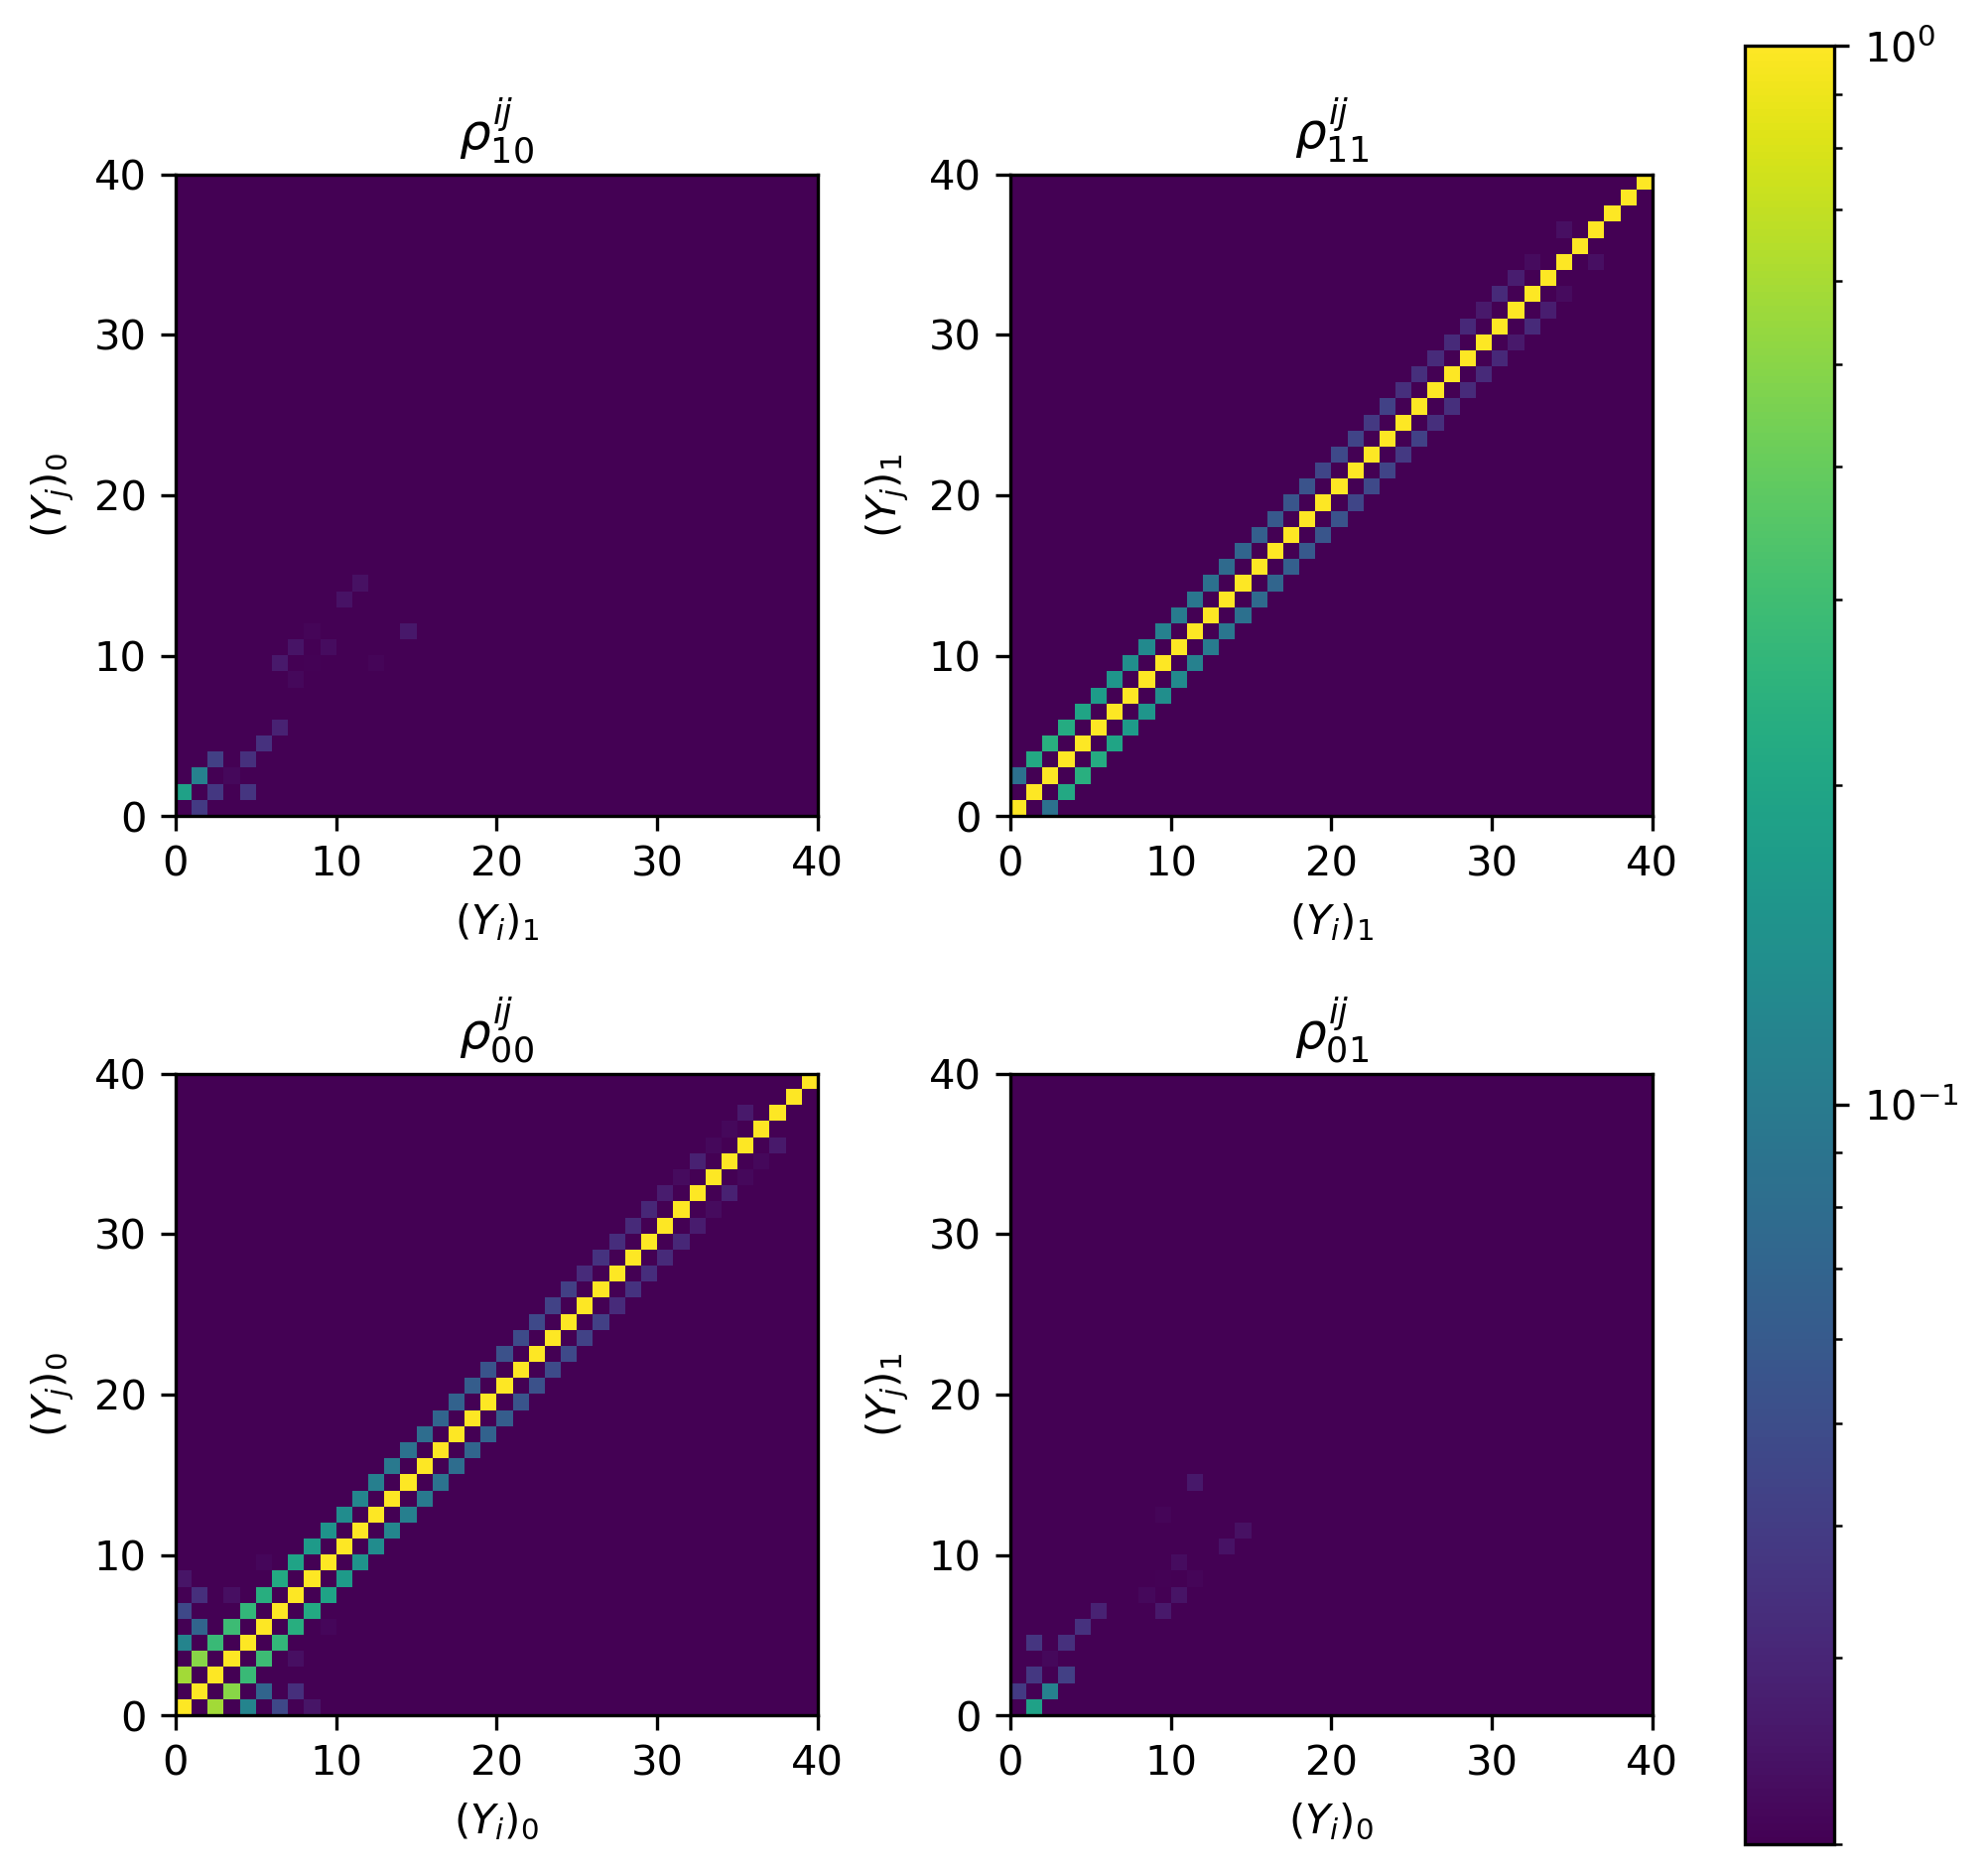
\includegraphics[width=0.66\textwidth]{figs_part1/mcmc/mode_convergence_covariance}
\centering \caption{The absolute normalised covariance $\rho_{kl}^{ij}=E^{\mathbb{P}}\left\{ (Y_{i})_{k}(Y_{j})_{l}\right\} /\sqrt{E^{\mathbb{P}}\left\{ (Y_{i})_{k}^{2}\right\} E^{\mathbb{P}}\left\{ (Y_{j})_{l}^{2}\right\} }$
of the modes of the sample paths in the KKL basis, found by sampling
the system with gradient dynamics using the TMC, at $\theta/\theta_{0}=3.36$,
$T/T_{0}=3$ and $N=200(T/T_{0})$.}
\label{fig:mode covariance} 
\end{figure}
\begin{figure}[t]
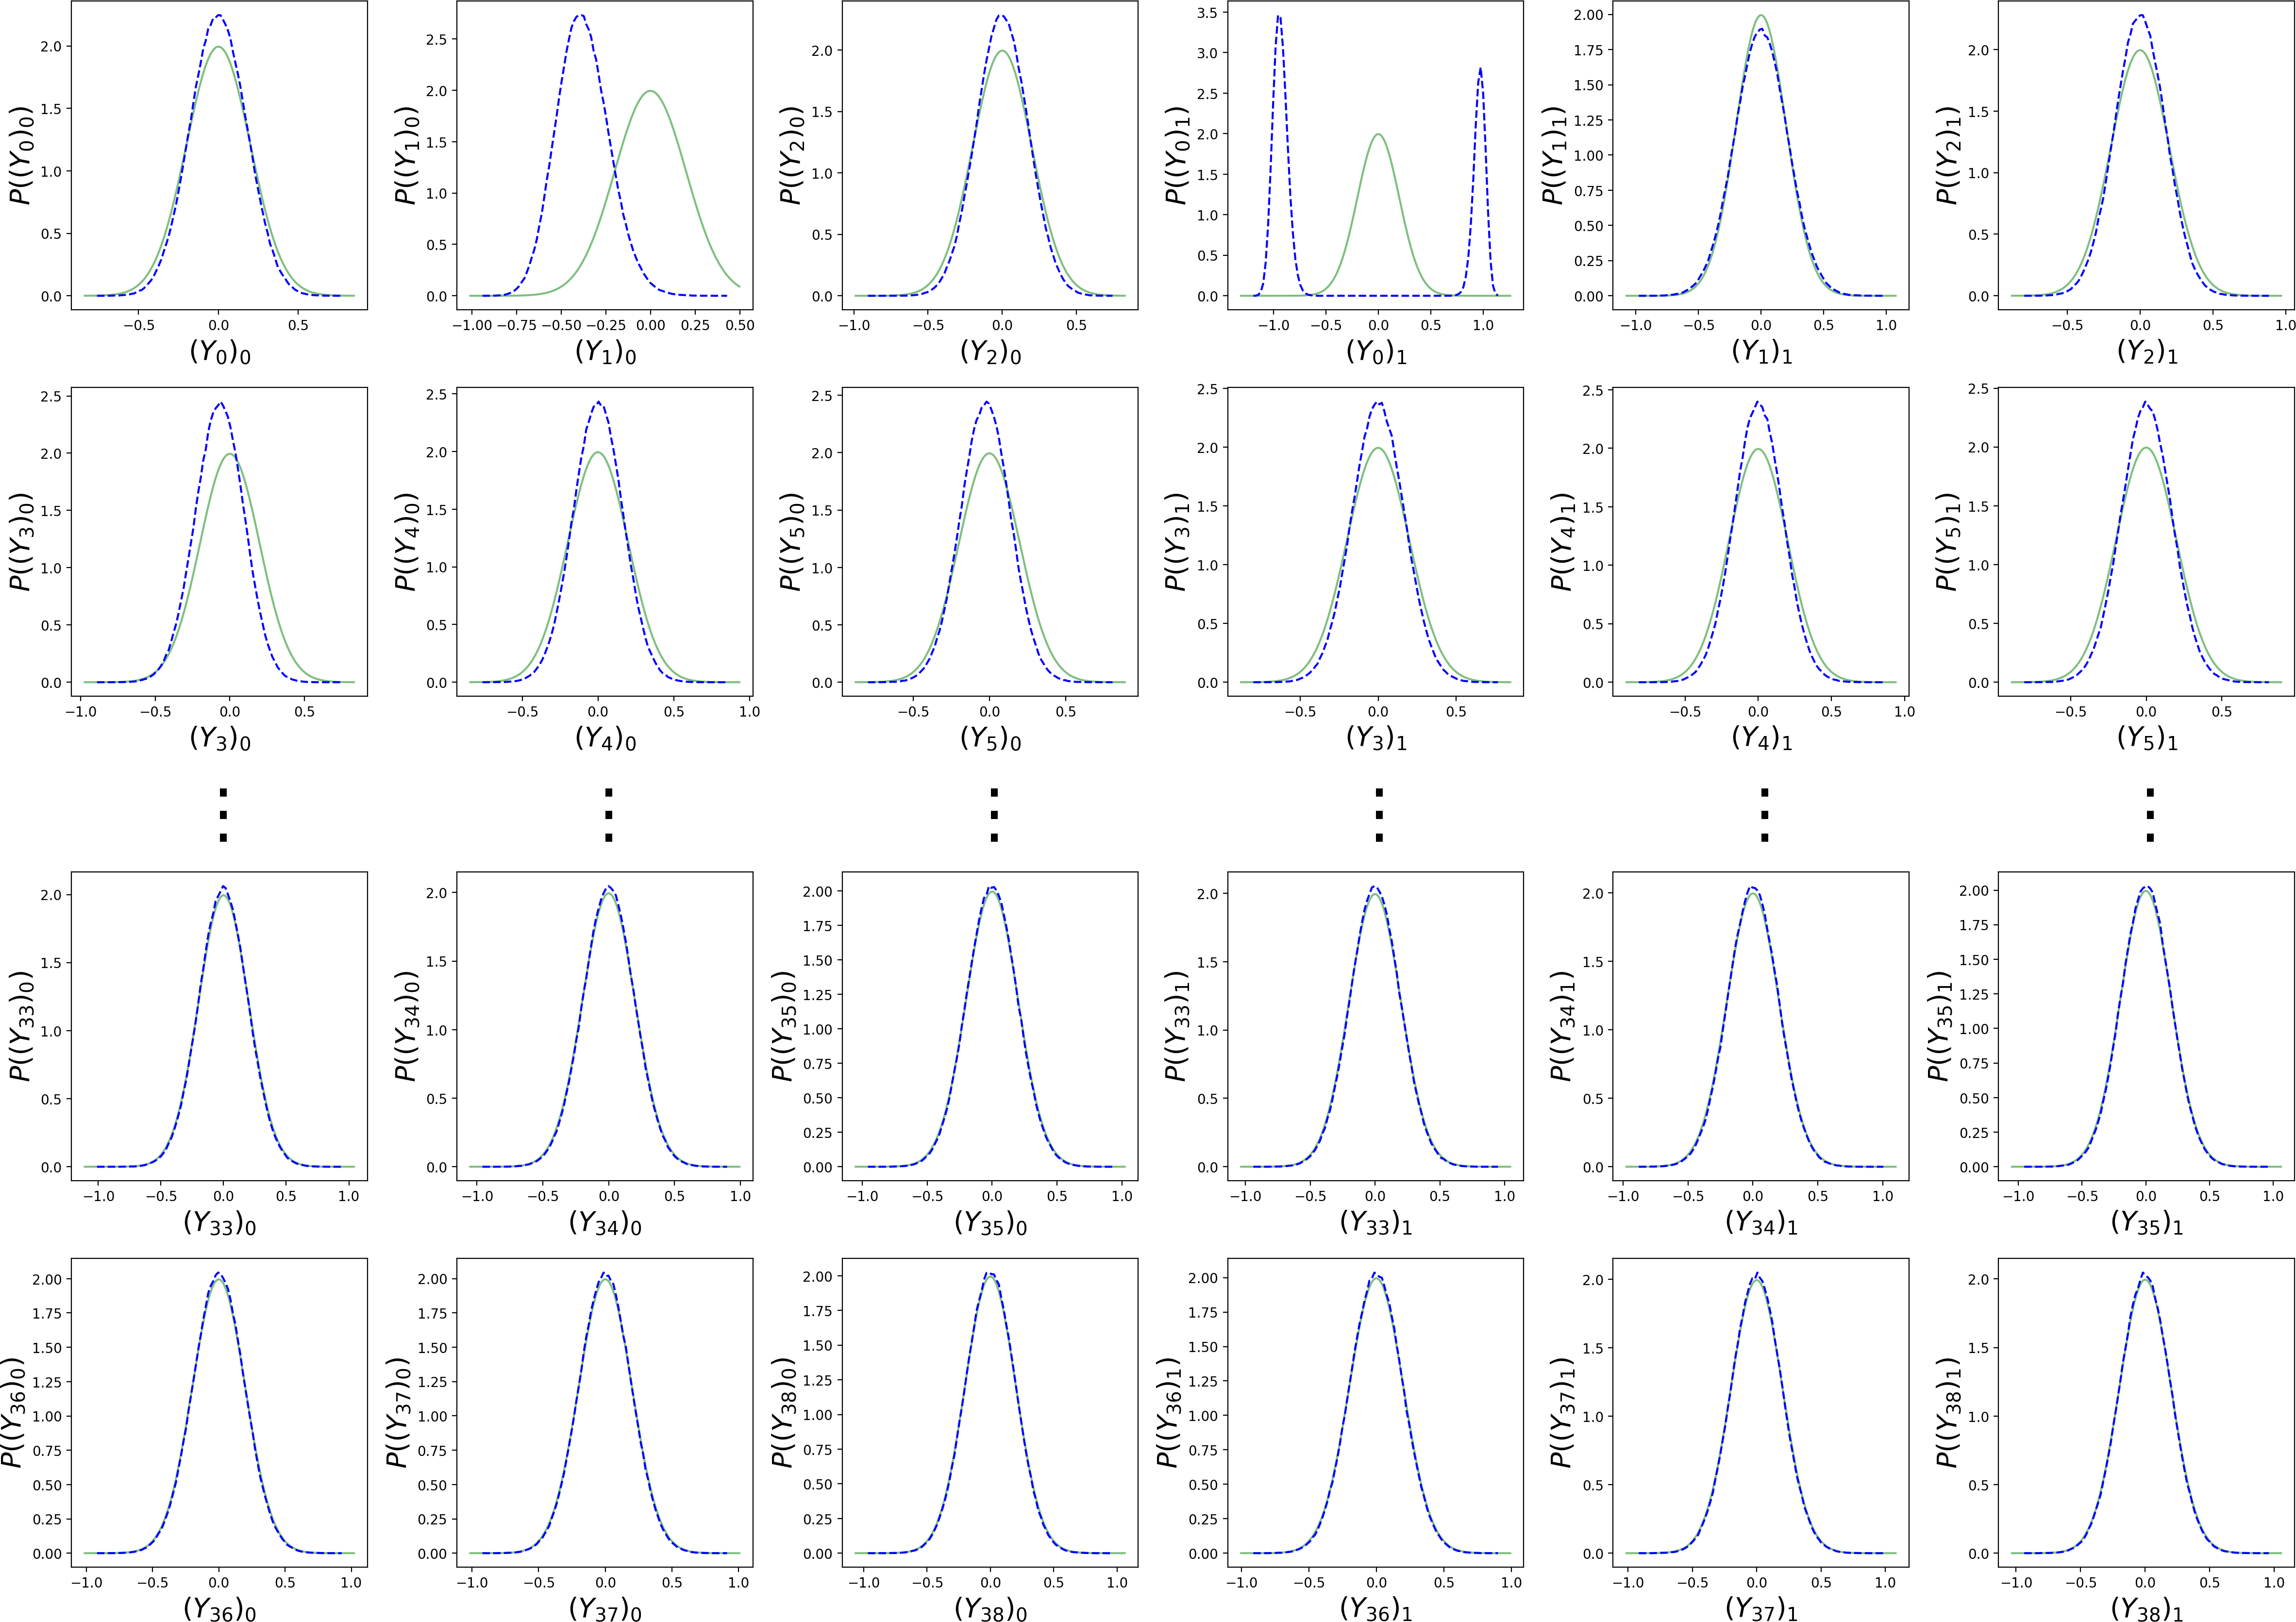
\includegraphics[width=1\textwidth]{figs_part1/mcmc/mode_convergence_marginalised}
\centering \caption{The marginalised distributions of the of the modes of the sample paths
(blue) and the Wiener process (green) in the KKL basis, found by sampling
the system with gradient dynamics using the TMC, at $\theta/\theta_{0}=3.36$,
$T/T_{0}=3$ and $N=200(T/T_{0})$.}
\label{fig:mode marginalised} 
\end{figure}
Here we describe in further detail the \emph{Teleporter MCMC }(TMC)
algorithm used in the main text. We start with a discussion of the
algorithm in its infinite dimensional form, defined directly on the
space of continuous paths, and then proceed to describe a modification
of the algorithm adapted to the KKL discretisation.

At each step of the MCMC, with a probability $p_{\text{teleport}}$,
we draw an independent proposal step $\mathbf{X}^{'}$ from the mixed
Gaussian distribution

\begin{equation}
\bar{\mathbb{P}}=\sum_{\alpha=1}^{K}w_{\alpha}\mathbb{\mathbb{P}}^{[\alpha]}\label{eq:mixed gaussian-1}
\end{equation}
where the weights $w_{\alpha}$ are parameters that must satisfy $\sum_{\alpha=1}^{K}w_{\alpha}=1$,
and where $\mathbb{\mathbb{P}}^{[\alpha]}$ are Gaussian distributions
with precision operators $\mathcal{H}^{[\alpha]}$ and mean $\bar{\mathbf{x}}$
as defined in previous sections. Using the Metropolis-Hastings condition
to ensure that the MCMC samples the target measure $\mathbb{P}$ of
the Itô process we find that $\mathbf{X}'$ should be accepted with
probability
\begin{equation}
a_{\text{TMC}}\left[\mathbf{X}',\mathbf{X}^{(n)}\right]=\min\left\{ 1,\exp\left(\Phi[\mathbf{X}^{(n)}]-\Phi[\mathbf{X}']\right)\frac{\sum_{\alpha}w_{\alpha}\exp\left(-\Psi^{[\alpha]}[\mathbf{X}^{(n)}]\right)}{\sum_{\alpha}w_{\alpha}\exp\left(-\Psi^{[\alpha]}[\mathbf{X}']\right)}\right\} \label{eq:acceptance probability}
\end{equation}
where $\mathbf{X}^{(n)}$ is current state of the MCMC, and $\Psi^{[\alpha]}$
is the logarithmic density of $\mathbb{P}^{[\alpha]}$ with respect
to the Wiener measure $\frac{d\mathbb{\mathbb{P}}^{[\alpha]}}{d\mathbb{P}_{W}}=\exp(-\Psi^{[\alpha]})$
and

\begin{align}
\Psi^{[\alpha]}[\mathbf{X}] & =\Psi_{1}^{[\alpha]}[\mathbf{X}-\mathbf{x}^{[\alpha]}]+\Psi_{2}^{[\alpha]}[\mathbf{X}]\\
\Psi_{1}^{[\alpha]}[\mathbf{X}] & =\int_{0}^{T}\left(2\mathbf{X}^{T}A(t)d\mathbf{X}+\mathbf{X}^{T}B(t)\mathbf{X}dt\right)\\
\Psi_{2}^{[\alpha]}[\mathbf{X}] & =\frac{\beta}{2\mu}\int_{0}^{T}\left(2\dot{\mathbf{x}}^{[\alpha]T}d\mathbf{X}-|\dot{\mathbf{x}}^{[\alpha]}|^{2}dt\right)
\end{align}
Thus far, the algorithm has been defined directly on the space of
continuous paths, but in numerical applications it is necessary to
apply a discretisation procedure. We can approximate $\mathbb{\mathbb{P}}^{[\alpha]}$
as a multivariate Gaussian by expanding its precision operator $\mathcal{H}^{[\alpha]}$
in the KKL basis \citep{kosambiParallelismPathspaces2016,karhunenUberLineareMethoden1947,loeveProbabilityTheory1977}
of the Wiener process as $\left(H_{ij}^{[\alpha]}\right)_{kl}=\langle\mathbf{e}_{k}\phi_{i},$$\mathcal{H}^{[\alpha]}\mathbf{e}_{l}\phi_{j}\rangle$,
$i,j=1,\dots,N$, $k,l=1,\dots,d$, where, $\mathbf{e}_{k}$ is a
constant vector with one non-zero component $(e_{k})_{l}=\delta_{kl}$.
Due to our discretisation procedure $M$ can be kept small as the
noise dominates over the drift for high-frequency modes, which manifests
itself as $H_{ij}^{[\alpha]}$ rapdily converging onto the precision
matrix of the Wiener measure , $\left(H_{ij}^{W}\right)_{kl}=\frac{\beta}{4\mu}\delta_{ij}\delta_{kl}$,
for high mode numbers $i,j$. This is demonstrated in Fig. \ref{fig:mode covariance}
and Fig. \ref{fig:mode marginalised}.

Using the multivariate Gaussian with precision matrix $\tilde{H}^{[\alpha]}$,
we construct a grafted Gaussian process ${\bf W}^{[\alpha]}(t)=\mathbf{x}^{[\alpha]}(t)+\sqrt{\frac{2\mu}{\beta}}\sum_{i=1}^{\infty}\mathbf{Z}_{i}^{[\alpha]}\sqrt{\lambda_{i}}\phi_{i}(t)$
where $(\mathbf{Z}_{1}^{[\alpha]},\dots,\mathbf{Z}_{M}^{[\alpha]})\sim\mathcal{N}(0,\tilde{H}^{[\alpha]})$
and $\mathbf{Z}_{i}^{[\alpha]}\sim\mathcal{N}(0,I_{d}),\ i>M$, where
$I_{d}$ is the $d$-dimensional identity matrix. This defines a Gaussian
measure $\mathbb{\tilde{P}}^{[\alpha]}$ on the space of stochasic
paths from which we can sample efficiently. Finally, we construct
a Gaussian mixture measure as the linear combination

\begin{equation}
\tilde{\mathbb{P}}=\sum_{\alpha=1}^{K}\tilde{w}_{\alpha}\mathbb{\tilde{P}}^{[\alpha]}\label{eq:mixed gaussian-1-1}
\end{equation}
from which we draw independent samples in the same manner as before.
The logarithmic densities of $\mathbb{\tilde{P}}^{[\alpha]}$ with
respect to the Wiener measure $\mathbb{P}_{W}$ are now

\begin{equation}
\tilde{\Psi}^{[\alpha]}[\mathbf{X}]=\sum_{i,j=1}^{M}\sum_{k,l=1}^{d}\frac{1}{2}(Y_{ik}-Y_{ik}^{[\alpha]})\tilde{K}_{ijkl}^{[\alpha]}(Y_{jl}-Y_{jl}^{[\alpha]})+2\sum_{i=1}^{M}\mathbf{Y}_{i}^{[\alpha]T}\mathbf{Y}_{i}+\sum_{i=1}^{M}\mathbf{Y}_{i}^{[\alpha]T}\mathbf{Y}_{i}^{[\alpha]}.
\end{equation}
where ${\bf X}(t)=\mathbf{x}_{0}+\bar{\mathbf{v}}t+\sqrt{\frac{2\mu}{\beta}}\sum_{i=1}^{\infty}\mathbf{Y}_{i}\sqrt{\lambda_{i}}\phi_{i}(t)$,
$Y_{ik}$ denotes the $k$th component of $\mathbf{Y}_{i,}$ $Y_{ik}^{[\alpha]}=\langle\mathbf{x}^{[\alpha]},\mathbf{e}_{k}\phi_{i}\rangle$,
$\left(\tilde{K}_{ij}^{[\alpha]}\right)_{kl}=\langle\mathbf{e}_{k}\phi_{i},(\mathcal{H}^{[\alpha]}-\mathcal{H}^{W})\mathbf{e}_{l}\phi_{j}\rangle$,
$\tilde{L}_{ik}^{[\alpha]}=\frac{\beta}{2\mu}$ using which the acceptance
probabilities are computed as in Eq.~\eqref{eq:acceptance probability}.

We now summarise the full algorithm, expressed in the KKL basis:

\begin{enumerate}

\item Choose an initial state $\mathbf{Y}^{(0)} \in \mathbb{R}^{N \times d}$.

\item Draw a random number $U^{(n+1)} \sim \text{Unif}([0,1])$.

\begin{itemize}

	\item If $U^{(i+1)} > p_\text{teleport}$.
		\begin{enumerate}
	
			\item Given state $\mathbf{Y}^{(n)}$, the $(n+1)$-th proposal is
				\begin{equation}
					\mathbf{Y}'_i = \sqrt{1 - \kappa^2} \mathbf{Y}_i^{(n)} + \kappa \mathbf{Z}_i^{(n)}
				\end{equation}
				where $\mathbf{Z}_i^{(n)} \sim \mathcal{N}(0,I_d)$ and $i=1,\dots,N$.
			
			\item Draw a random number $V^{(n+1)} \sim \text{Unif}([0,1])$.
			\begin{itemize}
				\item If $V^{(i+1)} < a[\mathbf{x}(t;\mathbf{Y}'), \mathbf{x}(t;\mathbf{Y}^{(n)})]$ then set $\mathbf{Y}^{(n+1)} = \mathbf{Y}'$.
				\item Otherwise set  $\mathbf{Y}^{(n+1)} = \mathbf{Y}^{(n)}$.
			\end{itemize}
	
		\end{enumerate}

	\item If $U^{(i+1)} \leq p_\text{teleport}$:

		\begin{enumerate}
			\item Given state $\mathbf{Y}^{(n)}$, the $(n+1)$-th proposal is
				\begin{equation}
					\mathbf{Y}'_i = \tilde{\mathbf{Z}}_{i}^{(n)}
				\end{equation}
				where $\tilde{\mathbf{Z}}^{(n)}$ is drawn from $\tilde{\mathbb{P}}_N$, and  $i=1,\dots,N$.
			
			\item Draw a random number $W^{(n+1)} \sim \text{Unif}([0,1])$.
			\begin{itemize}
				\item If $W^{(i+1)} < a_\text{TMC}[\mathbf{x}(t;\mathbf{Y}'), \mathbf{x}(t;\mathbf{Y}^{(n)})]$ then set $\mathbf{Y}^{(n+1)} = \mathbf{Y}'$.
				\item Otherwise set  $\mathbf{Y}^{(n+1)} = \mathbf{Y}^{(n)}$.
			\end{itemize}
		\end{enumerate}

\end{itemize}

\item Repeat step 2.

\end{enumerate}where $\text{Unif}([0,1])$ is the uniform distribution over the unit
interval, $\mathbf{x}(t;\mathbf{Y})=\mathbf{x}_{0}+\bar{\mathbf{v}}t+\sqrt{\frac{2\mu}{\beta}}\sum_{i=1}^{N}\mathbf{Y}_{i}\sqrt{\lambda_{i}}\phi_{i}(t)$,
and $\tilde{\mathbb{P}}_{N}$ is the truncation of Eq.~\eqref{eq:mixed gaussian-1-1}
to $N$ modes. In the numerical experiments discussed in the main
text, we used $\tilde{w}_{1}=\tilde{w}_{2}=1/2$ and $M=10(T/T_{0})$.

As mentioned in the main text, an alternate method to the above would
be a synthesis of the two sampling approaches in the above algorithm.
We could replace the reference Wiener measure $\mathbb{P}_{W}$ with
the mixed Gaussian $\tilde{\mathbb{P}}$, and thus perform the pCN-MCMC
with $\tilde{\mathbb{P}}$ as the invariant measure.


\subsection{Model system}

Here we define the two systems in consideration in the main text.
We construct a Sombrero-type potential such that the perpendicular
curvature of the potential along the minimal upper semi-circle $\Gamma^{+}$
is larger than that along the lower semi-circle $\Gamma^{-}$. We
start with a radial quartic potential of the form 
\begin{align}
U(x_{1},x_{2}) & =U_{r}(r(x_{1},x_{2}))\\
U_{r}(r) & =U_{0}\left(\frac{r}{L}-1\right)\left(1+a\frac{r}{L}+b\left(\frac{r}{L}\right)^{2}+c\left(\frac{r}{L}\right)^{3}\right)\nonumber 
\end{align}
where $L$ is the length-scale of the system, $U_{0}$ will be the
value of the potential at the local maximum $r=0$, and $a,b,c\in\mathbb{R}$
will be specified below. We will henceforth supress the argument of
the radial coordinate function $r(x_{1},x_{2})=\sqrt{x_{1}^{2}+x_{2}^{2}}$.
Let $\Gamma=\{(x,y)\ |\ r=1\}$ be the circle centered around the
origin, which satisfies $U_{r}(1)=0$. We also define $\Gamma^{+}$and
$\Gamma^{-}$ as the upper and lower semi-circle respectively. We
impose the following conditions on the potential to fix $a,b,c$:
\begin{enumerate}
\item $U_r'(0) = 0$. The origin is an extremum.
\item $U_r'(1) = 0$. $\Gamma$ is an extremum of the potential. \item $U_r''(1) = k$. The curvature along $\Gamma$ is $k$.
\end{enumerate}We get
\begin{equation}
U_{r}(r)=\frac{1}{2}\left(\frac{r}{L}-1\right)^{2}\left[L^{2}k\left(\frac{r}{L}\right)^{2}-2U_{0}\left(\frac{r}{L}-1\right)\left(3\frac{r}{L}+1\right)\right]
\end{equation}
In order to ensure that the potential has a Sombrero-like form, we
must further have that the potential is confining, which is equivalent
to $\underset{r\to\infty}{\lim}U_{r}(r)=\infty$, which implies that
$6U_{0}\leq L^{2}k$. We now introduce an angular dependence in the
curvature. We set
\begin{equation}
L^{2}k(\phi)=6U_{0}(1+2h(\phi))\label{eq:curvature}
\end{equation}
where $\phi=\phi(x_{1},x_{2})$ is the angle of $(x_{1},x_{2})$ in
polar coordinates so that $x_{1}=\cos(\phi)$, $x_{2}=\sin(\phi)$,
and where
\begin{equation}
h(\phi)=\frac{1}{4}\left(\xi_{2}+\xi_{1}+(\xi_{2}-\xi_{1})\sin\phi\right)
\end{equation}
where $\xi_{2}>\xi_{1}$, and where $h(\phi)\in[\xi_{1},\xi_{2}]$
satisfies $h(-\pi/2)=\xi_{1}$ and $h(\pi/2)=\xi_{2}$. Eq.~\eqref{eq:curvature}
is constructed so that the perpendicular curvature of $\Gamma^{+}$
is larger than that of $\Gamma^{-}$. The drift of the system is now
given by $\mathbf{F}=-\nabla U$.

For the non-gradient system, we introduce an additional non-conservative
force $\mathbf{F}^{a}=-\eta\hat{\boldsymbol{\phi}}$ for which the
work done in a displacement $d\mathbf{x}=dr\hat{\mathbf{r}}+rd\phi\hat{\boldsymbol{\phi}}$
is $dW=\mathbf{F}^{a}\cdot d\mathbf{x}=\eta rd\phi$. This force energetically
biases the upper transition channel $\Gamma^{+}$. The total force
is thus $\mathbf{F}=-\nabla U+\mathbf{F}^{a}$.

In the numerical experiments presented in the main text, we used the
Itô Langevin equation 

\begin{equation}
d\mathbf{X}=\mu\mathbf{F}dt+\sqrt{2\mu k_{B}\theta}d\mathbf{W}.\label{eq:langevin equation}
\end{equation}
We now put Eq. \ref{eq:langevin equation} in non-dimensionalised
form by introducing the time-scale $T_{0}=\frac{L^{2}}{k_{B}\theta_{0}\mu}$
and temperature-scale $\theta_{0}$, and setting $t=T_{0}\tilde{t}$,
$\theta=\theta_{0}\tilde{\theta}$, $\mathbf{X}=L\tilde{\mathbf{X}}$,
$\mathbf{F}=\frac{U_{0}}{L}\tilde{\mathbf{F}}$ and $\mathbf{W}=\sqrt{T_{0}}\tilde{\mathbf{W}}.$
$T_{0}$ is the typical diffusion time-scale at temperature $\theta_{0}$.
We get
\[
d\mathbf{\tilde{X}}=\tilde{U}_{0}\tilde{\mathbf{F}}d\tilde{t}+\sqrt{2\tilde{\theta}}d\tilde{\mathbf{W}}.
\]
where $\tilde{U}_{0}=\frac{U_{0}}{k_{B}\theta_{0}}$ is the ratio
of the well-depth $U_{0}$ and the thermal energy at temperature $\theta_{0}$.
For the numerical experiments in the main text  we use $\tilde{U}_{0}=1$,
which means that $\tilde{\theta}=1$ corresponds to a temperature
such that $k_{B}\theta=U_{0}$. We also set $\xi_{1}=0$ and $\xi_{2}=2$.
To compare the gradient force with $\mathbf{F}^{a}$ we also introduce
$f_{\text{eq}}=U_{0}/L$, which is the characteristic force strength
of the gradient force.



\subsection{Gaussian mixture approximation of the transition path ensemble}

Here we derive an approximation of the transition path ensemble, using
a Gaussian mixture approximation of the path-space probability measure.
The subsequent sections give detailed descriptions of the mathematical
techniques necessary for the approximation, but we will first give
some intuition by drawing an analogy to a one-dimensional probability
density.

For a one-dimensional probability density $\rho(x)=\mathcal{N}^{-1}\exp(-V(x))$,
where $\mathcal{N}$ is a normalization constant and where the potential
$V(x)$ has well-separated relative minima $x_{\alpha},\ \alpha=1,\dots,K$,
we can approximate $\rho(x)$ around $x_{\alpha}$ using a Gaussian
approximation
\begin{equation}
\rho(x)\approx\frac{1}{\mathcal{{N}}}e^{-V(x_{\alpha})-V''(x_{\alpha})(x-x_{\alpha})^{2}/2}=:\frac{{{\mathcal{N}}_{\alpha}}}{\mathcal{{N}}}e^{-V(x_{\alpha})}\rho^{[\alpha]}(x)\label{eq:local approximation of rho}
\end{equation}
with a normalised Gaussian distribution $\rho^{[\alpha]}(x):=\mathcal{N}_{\alpha}^{-1}e^{-V''(x_{\alpha})(x-x_{\alpha})^{2}/2}$
and where $\mathcal{N}_{\alpha}=\sqrt{2\pi/V''(x_{\alpha})}$. Equation
\ref{eq:local approximation of rho} is a local approximation of $\rho(x)$
around $x_{\alpha}$. If $\rho(x)$ is highly peaked around its maxima
(for example if $V(x)$ describes a Boltzmann distribution $V(x)=U(x)/(k_{B}\theta)$
at a low temperature $\theta$), a global approximation of $\rho(x)$
is the Gaussian mixture
\begin{equation}
\rho(x)\approx\sum_{\alpha=1}^{K}\frac{{\mathcal{{N}}}_{\alpha}}{\mathcal{{N}}}e^{-V(x_{\alpha})}\rho^{[\alpha]}(x)=:\sum_{\alpha=1}^{K}w_{\alpha}\rho^{[\alpha]}(x)\label{eq:one_dimensional_sum_of_gaussians}
\end{equation}
where $w_{\alpha}=e^{-V(x_{\alpha})}\mathcal{N}_{\alpha}/\mathcal{{N}}$
are constants that weight the local Gaussian distributions, and where
$\mathcal{N}\approx\sum_{\gamma=1}^{K}e^{-V(x_{\gamma})}\mathcal{N}_{\gamma}$. 

Equation \eqref{eq:one_dimensional_sum_of_gaussians} can be used
to approximately evaluate any expectation value. In particular, the
probability of being in well $\alpha$ (i.e.~around $x_{\alpha}$)
is given by

\begin{align}
P(x\in\text{{well\,}}\alpha) & =\mathbb{E}[\chi_{\alpha}]=\int_{-\infty}^{\infty}dx\,\chi_{\alpha}(x)\rho(x)\approx\sum_{\beta=1}^{K}w_{\beta}\int_{-\infty}^{\infty}dx\,\chi_{\alpha}(x)\rho^{[\beta]}(x)\\
 & \approx w_{\alpha}\int_{-\infty}^{\infty}dx\,\rho^{[\alpha]}(x)=w_{\alpha}=\frac{{e^{-V(x_{\alpha})}\mathcal{N}_{\alpha}}}{\sum_{\gamma=1}^{L}e^{-V(x_{\gamma})}\mathcal{N}_{\gamma}},\label{eq:one_dimensional_well_probability}
\end{align}
where the indicator function $\chi_{\alpha}(x)$ is 1 if $x$ is in
well $\alpha$ and zero otherwise, and where we assume that the potential
wells of $V(x)$ are well-separated so that $\chi_{\alpha}(x)\rho^{[\beta]}(x)$
is negligibly small whenever $\alpha\neq\beta$.

In the following we apply the same steps as above to the case of the
transition path ensemble (TPE). As we are considering Gaussian approximations
of probability distributions over infinite-dimensional functional
spaces, the mathematical sophistication required is higher, but the
intuition remains identical to the above one-dimensional example.
In Sec.~II.A we derive the local Gaussian approximation for path-probability
measures around an instanton (which is based on a second-order functional
Taylor approximation), which we in Sec.~II.B combine to a Gaussian
mixture approximation of the TPE. In Sec.~II.D we derive the method
we use to calculate the normalisation constants for functional Gaussians
(i.e. the infinite-dimensional equivalent of the $\mathcal{N}_{\alpha}$
from the one-dimensional example above). We put Sec.~II.D last as
it is a technical result, and is not required to understand the rest
of the subsections. In Sec.~II.C we use the Gaussian mixture to derive
an approximate expression for transition pathway probabilities, which
proceeds analogous to the calculation Eq.~\eqref{eq:one_dimensional_well_probability}.

\subsection{The quadratic expansion of the Onsager-Machlup action}

Here we describe how to formally construct the Gaussian expansion
around a given reference path. The variational expansion of the Onsager-Machlup
action

\begin{align}
S_{\text{OM}}[\mathbf{x}(t)] & =\int_{0}^{T}L(\mathbf{x}(t),\dot{\mathbf{x}}(t))dt\label{eq:onsager-machlup action}\\
L(\mathbf{x},\dot{\mathbf{x}}) & =\frac{\beta}{4\mu}|\dot{{\bf x}}-\mathbf{F}|^{2}+\frac{\mu}{2}\nabla\cdot\mathbf{F}\nonumber 
\end{align}
where $\beta=1/k_{B}\theta$ is the inverse temperature, is given
by
\begin{align}
S_{\text{OM}}[\mathbf{\mathbf{\bar{\mathbf{x}}}}+\delta\mathbf{x}] & =S_{\text{OM}}[\mathbf{\mathbf{\bar{\mathbf{x}}}}]+\mathrm{J}[\delta\mathbf{x}]+\frac{1}{2}\mathrm{H}[\delta\mathbf{x}]+O(\delta\mathbf{x}^{3})\label{eq:variation of OM}
\end{align}
to second order around a reference path $\mathbf{\bar{\mathbf{x}}}(t)$,
where
\begin{align}
\mathrm{J}[\delta\mathbf{x}] & =\int_{0}^{T}\left\{ \frac{\partial L}{\partial\mathbf{x}}(\mathbf{\mathbf{\bar{\mathbf{x}}}},\dot{\mathbf{\mathbf{\bar{\mathbf{x}}}}})\cdot\delta\mathbf{x}+\frac{\partial L}{\partial\dot{\mathbf{x}}}(\mathbf{\mathbf{\bar{\mathbf{x}}}},\dot{\mathbf{\mathbf{\bar{\mathbf{x}}}}})\cdot\delta\dot{\mathbf{x}}\right\} dt\\
\mathrm{H}[\delta\mathbf{x}] & =\int_{0}^{T}\left\{ \delta\mathbf{x}\cdot\frac{\partial^{2}L}{\partial\mathbf{x}\partial\mathbf{x}}(\mathbf{\mathbf{\bar{\mathbf{x}}}},\dot{\mathbf{\mathbf{\bar{\mathbf{x}}}}})\cdot\delta\mathbf{x}+2\ \delta\mathbf{x}\cdot\frac{\partial^{2}L}{\partial\mathbf{x}\partial\dot{\mathbf{x}}}(\mathbf{\mathbf{\bar{\mathbf{x}}}},\dot{\mathbf{\mathbf{\bar{\mathbf{x}}}}})\cdot\delta\dot{\mathbf{x}}+\delta\dot{\mathbf{x}}\cdot\frac{\partial^{2}L}{\partial\dot{\mathbf{x}}\partial\dot{\mathbf{x}}}(\mathbf{\mathbf{\bar{\mathbf{x}}}},\dot{\mathbf{\mathbf{\bar{\mathbf{x}}}}})\cdot\delta\dot{\mathbf{x}}\right\} dt.\label{eq:functional Q}
\end{align}
In the following we will suppress the arguments of the derivatives
of the Lagranian. We will now recast Eq.~\eqref{eq:variation of OM}
in terms of self-adjoint operators using integration-by-parts and
$\delta\mathbf{x}(0)=\delta\mathbf{x}(T)=0$. We also note that $\left\langle \mathbf{f},P\frac{d}{dt}\mathbf{g}\right\rangle =-\left\langle \frac{d}{dt}\left(P^{T}\mathbf{f}\right),\mathbf{g}\right\rangle $,
for any matrix function $P(t)\in\mathbb{R}^{d\times d}$, and where
$\langle\mathbf{f},\mathbf{g}\rangle=\sum_{i}\int_{0}^{T}f_{i}(t)g_{i}(t)dt$,
which we use to symmetrise the second term in Eq.~\eqref{eq:functional Q}.
We get

\begin{equation}
S_{\text{OM}}[\bar{\mathbf{x}}+\delta\mathbf{x}]=S_{\text{OM}}[\bar{\mathbf{x}}(t)]+\langle\mathbf{j},\delta\mathbf{x}\rangle+\frac{1}{2}\langle\delta\mathbf{x},\mathcal{H}\delta\mathbf{x}\rangle+O(\delta\mathbf{x}^{3})\label{eq:OM expansion in operator form}
\end{equation}
where
\begin{align}
\mathbf{j}(t) & =\frac{\partial L}{\partial\mathbf{x}}-\frac{d}{dt}\frac{\partial L}{\partial\dot{\mathbf{x}}}\label{eq:euler-lagrange}\\
\mathcal{\mathcal{H}} & =-\frac{\beta}{2\mu}\frac{d^{2}}{dt^{2}}+2A(t)\frac{d}{dt}+B(t)\label{eq:Q operator}
\end{align}
and $A_{ij}(t)=\frac{\partial^{2}L}{\partial x_{[i}\partial\dot{x}_{j]}}$,
$B_{ij}(t)=\frac{\partial^{2}L}{\partial x_{i}\partial x_{j}}-\frac{d}{dt}\frac{\partial^{2}L}{\partial x_{j}\partial\dot{x}_{i}}$,
where closed brackets indicate an anti-symmetrisation over indices.
By completing the square, we find that Eq.~\eqref{eq:OM expansion in operator form}
defines a Gaussian process $\delta\mathbf{x}\sim\mathcal{N}(-\mathcal{H}^{-1}\mathbf{j},\mathcal{H}^{-1})$,
which describes the quadratic fluctuations around $\bar{\mathbf{x}}$.
In the sense of \citep{grossAbstractWienerSpaces1967}, the path-space
density of the Gaussian process is $\rho[\delta\mathbf{x}]\propto\exp(-\frac{1}{2}\langle\delta\mathbf{x}+\mathcal{H}^{-1}\mathbf{j},\mathcal{H}(\delta\mathbf{x}+\mathcal{H}^{-1}\mathbf{j})\rangle)$.
If the reference path solves the Euler-Lagrange equation Eq.~\eqref{eq:onsager-machlup action},
then $\mathbf{j}=0$ and the Gaussian process simplifies to $\rho[\delta\mathbf{x}]\propto\exp(-\frac{1}{2}\langle\delta\mathbf{x},\mathcal{\mathcal{\mathcal{H}}}\delta\mathbf{x})\rangle)$.

For systems with gradient dynamics $\mathbf{F}=-\nabla U$, the asymmetric
term in Eq.~\eqref{eq:Q operator} vanishes, and the form of the
operator simplifies to 
\begin{equation}
\mathcal{\mathcal{H}}=-\frac{\beta}{2\mu}\frac{d^{2}}{dt^{2}}+B(t)\label{eq:Q operator gradient}
\end{equation}

\subsection{The Gaussian mixture approximation}

We now use the quadratic expansion of the Onsager-Machlup action to
construct an approximate probability measure over the TPE. \textit{\emph{Let
$\mathbf{x}^{[\alpha]},\alpha=1,\dots,K$ be the local instantons
of a given Langevin system. For each local instanton we can define
a Gaussian measure $\mathbb{P}^{[\alpha]}$ with mean $\mathbf{x}^{[\alpha]}$
and precision $H^{[\alpha]}$. Although the measure $\mathbb{P}^{[\alpha]}$
is defined over the space of $C^{0}$ continuous paths, the distribution
can be characterised via a density on the Hilbert space of $C^{2}$
paths as $\rho^{[\alpha]}[\mathbf{x}]\propto\exp(-\langle\mathbf{x}-\mathbf{x}^{[\alpha]},\mathcal{H}^{[\alpha]}(\mathbf{x}-\mathbf{x}^{[\alpha]})\rangle)$
}}\citep{grossAbstractWienerSpaces1967,FunctionalIntegrationBasics}\textit{\emph{.
To approximate the TPE distribution, we construct the mixed Gaussian
density $\bar{\rho}[\mathbf{x}]\propto\sum_{\alpha=1}^{K}e^{-S_{\text{OM}}[\mathbf{x}^{[\alpha]}]}\rho^{[\alpha]}[\mathbf{x}]$.
The normalisation constant $\mathcal{N}^{[\alpha]}$ of the densities
$\rho^{[\alpha]}[\mathbf{x}]$ are not finite, but can be expressed
as ratios with respect to the normalisation of the reference Wiener
measure $\mathcal{N}^{W}$. This ratio can be shown to be equal to
\citep{levitTheoremInfiniteProducts1977,dunneFunctionalDeterminantsQuantum2008}
\begin{equation}
\mathcal{Z}^{[\alpha]}:=\frac{\mathcal{N}^{[\alpha]}}{\mathcal{N}^{W}}=\left(\frac{\det[\mathcal{H}^{[\alpha]}]}{\det[-\frac{\beta}{2\mu}\frac{d^{2}}{dt^{2}}]}\right)^{-1/2}\label{eq:normalisation}
\end{equation}
where the RHS can be computed using the results in the Sec.}}~\textit{\emph{II-C.
Using Eq.}}~\textit{\emph{\eqref{eq:normalisation} we can write
down the approximation of the TPE as the Gaussian mixture \citep{gelmanBayesianDataAnalysis}
\begin{equation}
\mathbb{\bar{P}}=\sum_{\alpha=1}^{K}w_{\alpha}\mathbb{P}^{[\alpha]}\label{eq:TPE approximation}
\end{equation}
where $w_{\alpha}=e^{-S_{\text{OM}}[\mathbf{x}^{[\alpha]}]}\mathcal{Z}^{[\alpha]}/\sum_{\gamma=1}^{K}e^{-S_{\text{OM}}[\mathbf{x}^{[\gamma]}]}\mathcal{Z}^{[\gamma]}$.}}

\subsection{Approximations of transition channel probabilities}

We now derive an approximation to the probabilities of reactive pathways
using the Gaussian mixture approximation of the TPE. Let $\mathrm{E}_{\alpha}\subset C^{0},\alpha=1,\dots,K$,
which are disjoint open sets in the TPE, be the $K$ reactive pathways
under consideration. We define the observable
\begin{equation}
P^{[\alpha]}(\theta,T)=\mathbb{P}[E_{\alpha}]
\end{equation}
which is the probability of observing a path in $E_{\alpha}$. In
low temperatures we can assume that $\mathbb{P}(\cup_{\alpha}E_{\alpha})\approx1$,
i.e. approximately all stochastic paths transition via one of the
reactive pathways. Furthermore, we assume that $\mathbf{x}^{[\alpha]}\in E_{\alpha}$
and that $\mathbb{P}^{[\alpha]}(\cup_{\gamma\neq\alpha}E_{\gamma})\approx0$.
The latter assumption means that each measure $\mathbb{P}^{[\alpha]}$
is concentrated on $E_{\alpha}$ and lacks support on the other reactive
pathways. Under these assumptions we can approximate $P^{[\alpha]}(\theta,T)$
as
\begin{equation}
P^{[\alpha]}(\theta,T)\approx P_{G}^{[\alpha]}(\theta,T)\equiv w_{\alpha}.
\end{equation}


\subsection{Calculation of the Gaussian normalisation constants}

The regularised normalisation constants of Gaussians defined on functional
spaces can be found by computing the determinants of their covariance
operators. Equivalently, the normalisation can be found by computing
the determinant of their precision operator, which is the inverse
of the covariance operator. As for finite-dimensional linear operators,
determinants of differential operators can be found by computing their
eigenvalues, but this is in general a prohibitevely expensive computational
procedure. In the following we show that functional determinants,
acting on $d$-dimensional vectors, can be found by solving $d$ initial
value ODEs.

Let the linear operators
\begin{equation}
\mathcal{L}=\frac{d}{dt}\left(P\frac{d}{dt}\right)-R\label{eq:linear operator}
\end{equation}
and
\begin{equation}
\mathcal{L}_{0}=\frac{d}{dt}\left(P\frac{d}{dt}\right)\label{eq:free linear operator}
\end{equation}
be defined for $0\leq t\leq T$, and where $P(t)\in\mathbb{R}^{d\times d}$
is a positive-definite matrix function and $R(t)\in\mathbb{R}^{d\times d}$
is a matrix function. Let $\gamma^{(k)}$ and $\mathbf{u}^{(k)}(t;\alpha)$
be the eigenvalues and eigenfunctions of $\mathcal{L}$, which are
solutions to the boundary value problem
\begin{equation}
\mathcal{L}\mathbf{u}^{(k)}(t)=\gamma^{(k)}\mathbf{u}^{(k)}(t)\label{eq:eigenfunction eq}
\end{equation}
where $\mathbf{u}^{(k)}(0)=\mathbf{u}^{(k)}(T)=0$. Similarly, let
$\mathbf{u}_{0}^{(k)}(t)$ and $\gamma_{0}^{(k)}$ be the eigenfunctions
and eigenvalues of $\mathcal{L}_{0}$. Then the \emph{functional determinant}
of $\mathcal{L}$ is defined in regularised form as
\begin{equation}
\frac{\det\mathcal{L}}{\det\mathcal{L}_{0}}=\prod_{k=1}^{\infty}\frac{\gamma^{(k)}}{\gamma_{0}^{(k)}}.\label{eq:functional determinant}
\end{equation}
As the spectrum of Eq.~\eqref{eq:linear operator} is unknown, and
numerically expensive to compute, a much more efficient way of computing
Eq.~\eqref{eq:functional determinant} is via the Gelfand-Yaglom
theorem (GYT) \textit{\emph{\citep{gelfandIntegrationFunctionalSpaces1960,levitTheoremInfiniteProducts1977,dunneFunctionalDeterminantsQuantum2008}.
The GYT states that the functional determinant can be expressed as
\begin{equation}
\left|\frac{\det\mathcal{L}}{\det\mathcal{L}_{0}}\right|=\left|\frac{\det\left[Y(T)\right]}{\det\left[Y_{0}(T)\right]}\right|\label{eq:GY result}
\end{equation}
where $Y(t)\in\mathbb{R}^{d\times x}$ with components $Y_{ij}(t)=y_{i}^{(j)}(t)$,
where the $\mathbf{y}^{(j)}(t)$ are solutions to the $d$ second-order
ODEs with initial conditions}}

\begin{align}
\mathcal{L}\mathbf{y}^{(j)}(t) & =0\label{eq:GY theorem}\\
\mathbf{y}^{(j)}(0) & =0\\
\frac{d}{dt}y_{i}^{(j)}(0) & =\delta_{ij}.
\end{align}
\textit{\emph{and where the matrix $Y_{0}(t)\in\mathbb{R}^{d\times d}$
is defined similarly, but with $\mathcal{L}$ in Eq.}}~\textit{\emph{\eqref{eq:GY theorem}
replaced with $\mathcal{L}_{0}$.}}

In the case of gradient dynamics, where $\mathcal{H}$ takes the form
in Eq.~\eqref{eq:Q operator gradient}, the GYT can be readily applied
by setting $P(t)=-\frac{\beta}{2\mu}I_{d}$ and $R(t)=-B(t)$, where
$I_{d}$ is the identity matrix. We now present a generalisation of
the GYT that allows for linear operators of the form

\begin{equation}
\mathcal{L}=\frac{d^{2}}{dt^{2}}+U\frac{d}{dt}+R\label{eq:linear operator with 1st order term}
\end{equation}
where $0\leq t\leq T$, and where $U(t),\ R(t)\in\mathbb{R}^{d\times d}$
are matrix functions, which then makes the GYT applicable for systems
non-gradient dynamics, with precision operators of the form Eq.~\eqref{eq:Q operator}.

We define the linear operator $\mathcal{G}$ which acts on vector
functions as
\[
\mathcal{G}\mathbf{y}=G\mathbf{y}
\]
where $G(t)$ is a matrix function that solves the equation

\begin{equation}
\dot{G}=-\frac{1}{2}UG,\label{eq:G eq}
\end{equation}
then the linear operator
\begin{equation}
\tilde{\mathcal{L}}=\mathcal{G}^{-1}\mathcal{L}\mathcal{G}=\frac{d}{dt^{2}}+G^{-1}\left(R-\frac{1}{2}\dot{U}-\frac{1}{4}U^{2}\right)G\label{eq:H tilde}
\end{equation}
is of the form Eq.~\eqref{eq:linear operator} and $\det\tilde{\mathcal{L}}$
can then be computed using the GYT. As for any two operators $\mathcal{A}$
and $\mathcal{B}$, we have that $\det\mathcal{A\mathcal{B}}=\det\mathcal{A}\det\mathcal{B}$,
and $\det\mathcal{A}^{-1}=1/\det\mathcal{A}$, and we therefore have
that $\det\mathcal{L}=\det\tilde{\mathcal{L}}$. The functional determinant
$\det\mathcal{L}$ can thus be computed by first solving Eq.~\eqref{eq:G eq},
constructing $\tilde{\mathcal{L}}$ using Eq.~\eqref{eq:H tilde},
and finally using the GYT to compute $\det\tilde{\mathcal{L}}$.

The above theorem can be applied to Eq. \eqref{eq:Q operator} by
setting $P(t)=-\frac{\beta}{2\mu}I_{d}$, $U=-\frac{4\mu}{\beta}A$
and $R=B$. Using the GYT, and its generalisation presented here,
the problem of computing the normalisation constants of Gaussian distributions
in functional spaces is reduced to solving $d$ initial value problems.


{\color{red}

The TPE is characterized
by its corresponding probability measure $\mathbb{P}$ on the space
of all continuous transition paths. In the path-integral formalism,
this measure is represented by a formal density $\rho[\mathbf{x}(t)]=\exp(-S_{\text{OM}}[\mathbf{x}(t)])$
with respect to a fictitious infinite-dimensional Lebesgue measure
\citep{takahashiProbabilityFunctionalsOnsagermachlup1981}, with the
Onsager-Machlup action \citep{onsagerFluctuationsIrreversibleProcesses1953,bachFunctionalsPathsDiffusion1977,itoProbabilisticConstructionLagrangean1978}
\begin{equation}
S_{\text{OM}}[\mathbf{x}(t)]=\int_{0}^{T}\left(\frac{\beta}{4\mu}|\dot{{\bf x}}-\mathbf{F}|^{2}+\frac{\mu}{2}\nabla\cdot\mathbf{F}\right)dt.\label{eq:onsager-machlup action}
\end{equation}
The variational minima of the action Eq.~\eqref{eq:onsager-machlup action}
have physical relevance. Namely, because the first term in Eq.~\eqref{eq:onsager-machlup action}
is inversely proportional to the temperature, at sufficiently low
temperature the formal probability density $\rho$ is dominated by
paths that aggregate around the variational minima \citep{ventselSMALLRANDOMPERTURBATIONS1970,stratonovichMarkovMethodsTheory1989,grahamMacroscopicPotentialsBifurcations1989}.
These variational minima are called the local instantons of the Onsager-Machlup
action, and we denote them by $\mathbf{x}^{[\alpha]}(t;\ \theta,T)$,
with $\alpha=1,\dots,K$, $\mathbf{x}^{[\alpha]}(0;\ \theta,T)=\mathbf{x}_{0}$
and $\mathbf{x}^{[\alpha]}(T;\ \theta,T)=\mathbf{x}_{T}$. The arguments
of the local instantons indicate that they depend on the temperature
and the duration of the path (we suppress these arguments below).
For the potential $U$ from Fig.~\ref{fig:switch} (a) we find $K=2$
local instantons $\mathbf{x}^{[1]}\equiv\mathbf{x}^{+}$, $\mathbf{x}^{[2]}\equiv\mathbf{x}^{-}$,
going along the upper and lower semi-circles, respectively.

By performing a quadratic functional Taylor expansion of Eq.~\eqref{eq:onsager-machlup action}
around the $\alpha$-th local instanton \citep{engelDensityFunctionalTheory2011,gelfandCalculusVariations2012,corazzaNormalizedGaussianPath2020a},

\begin{equation}
S_{\text{OM}}[\mathbf{x}(t)]\approx S_{\text{OM}}[\mathbf{x}^{[\alpha]}(t)]+\frac{1}{2}\langle\delta\mathbf{x},\mathcal{H}^{[\alpha]}\delta\mathbf{x\rangle},\label{eq:quadratic expansion}
\end{equation}
where $\mathcal{H}^{[\alpha]}$ is a self-adjoint linear differential
operator, $\delta\mathbf{\mathbf{x}}=\mathbf{x}-\mathbf{x}^{[\alpha]}$
and $\langle\mathbf{f},\mathbf{g}\rangle=\sum_{i}\int_{0}^{T}f_{i}(t)g_{i}(t)dt$,
we can formally define a Gaussian measure $\mathbb{P}^{[\alpha]}$
with mean $\mathbf{x}^{[\alpha]}$, precision $\mathcal{H}^{[\alpha]}$,
\textit{\emph{and regularised normalisation constant $\mathcal{Z}^{[\alpha]}$,
}}in the space of paths. The resulting $K$ local approximators of
the measure can be combined into a Gaussian mixture approximation
\textit{\emph{\citep{gelmanBayesianDataAnalysis}}} of the whole TPE
\begin{equation}
\mathbb{P}\approx\bar{\mathbb{P}}\equiv\sum_{\alpha=1}^{K}w_{\alpha}\mathbb{P}^{[\alpha]},\label{eq:gaussian mixture approximation of TPE}
\end{equation}
where the weights $w_{\alpha}=e^{-S_{\text{OM}}[\mathbf{x}^{[\alpha]}]}\mathcal{Z}^{[\alpha]}/\sum_{\gamma=1}^{K}e^{-S_{\text{OM}}[\mathbf{x}^{[\gamma]}]}\mathcal{Z}^{[\gamma]}$
satisfy $\sum_{\alpha=1}^{K}w_{\alpha}=1$, see the SI \citep{note:SI}
for more details. Equation \eqref{eq:gaussian mixture approximation of TPE}
is the infinite-dimensional analogue to approximating a finite-dimensional
multimodal probability density by a sum of Gaussians, with one term
for each local maximum of the probability density.

}


{
\color{blue}

In the numerical verificaiton, show comparison of teleporter with switch and also with biased teleporters.

Also show an example where you compare FW to OM.
}



\section{Conclusion}

Restate main differences between TPS

Field stuff here



\chapter{Diffusivity dependence of transition paths} \label{ch:Diffusivity dependence of transition paths}

\section{Introduction}


The fluctuating dynamics of many physical, chemical and biological
systems are commonly modelled by stochastic differential equations
expressed in Langevin or Itô forms \citep{kampenStochasticProcessesPhysics2011,gardinerStochasticMethodsHandbook2010,riskenFokkerPlanckEquationMethods2012,bharucha-reidElementsTheoryMarkov2012}.
In such systems it is often of great interest to identify the typical
pathways that stochastic paths take to transition from an initial
to a final state, as for example in the nucleation of solids, the
conformational changes in biomolecules, or shifts in ecological balance
\citep{faccioliDominantPathwaysProtein2006, demarcoPhaseTransitionModel2001, gardnerConstructionGeneticToggle2000, mangelBarrierTransitionsDriven1994, wolynesNavigatingFoldingRoutes1995, huangMolecularMathematicalBasis2012, paninskiMostLikelyVoltage2006, noltingBallsCupsQuasipotentials2016, leeFindingMultipleReaction2017}.
Typically, such transition paths cluster around multiple pathways
in the space of configurations and the relative probability of one
or the other of these pathways depends on the drift, the diffusivity,
and the duration allowed for the transition to take place \citep{onsagerFluctuationsIrreversibleProcesses1953,bachFunctionalsPathsDiffusion1977,itoProbabilisticConstructionLagrangean1978,ikedaStochasticDifferentialEquations2014}.
As transitions are often rare events, direct simulations are not always
practical and other means, analytical or numerical, are required to
study them. Methods that allow for a full exploration of the space
of transition pathways in stochastic dynamical systems, then, are
of substantial theoretical and practical importance.

The theory of large deviations \citep{ventselSMALLRANDOMPERTURBATIONS1970,stratonovichMarkovMethodsTheory1989,grahamMacroscopicPotentialsBifurcations1989,arnoldStochasticDifferentialEquations1974}
provides an analytical method for obtaining transition pathways -
instantons - in regimes dominated by the drift and for very long durations
of path. Experimental systems, however, are typically not in a regime
where the diffusivity is asymptotically low and durations are asymptotically
long \citep{gladrowExperimentalMeasurementRelative2021}. While the
relevance of including finite-temperature fluctuations around the
instanton \citep{gelfandIntegrationFunctionalSpaces1960} is increasingly
recognized \citep{nickelsen_noise_2022,corazza_normalized_2020,lu_gaussian_2017},
the physical implications of these fluctuations are far from being
understood.

In this chapter, we show that the competition between drift and diffusion
in transition pathways can be studied using semi-classical expansions
of the path measure of the stochastic dynamics. We use a mixture of
Gaussian measures to approximate the path measure around its local
instantons. This allows us to demarcate and transcend the boundaries
of the low diffusivity regime. We demonstrate this explicitly for
a two-dimensional overdamped mechanical system, with both conservative
and non-conservative forces. For this system we uncover a counterintuitive
phenomenon where typical transition paths do not concentrate around
the most probable path, even at low-to-intermediate diffusivities
where the Gaussian approximation is still valid. To validate our results
numerically, we construct a Markov Chain Monte Carlo (MCMC) method
that allows for simultaneous exploration of multiple transition pathways.We
find excellent agreement between the semi-classical expansion and
numerical results for a large range of diffusivities and path durations.
We now detail our results.


\section{The transition path ensemble}

We consider the stochastic process
generated by the $d$-dimensional overdamped Langevin equation, expressed
in Itô form as
\begin{equation}
d\mathbf{X}=\mu\mathbf{F}dt+\sqrt{2D}d\mathbf{W}.\label{eq:ito equation}
\end{equation}
This represents the stochastic displacement $d\mathbf{X}$ in a time
interval $dt$ of a particle with coordinate $\mathbf{X}$ subject
to a force field $\mathbf{F}$ and Brownian displacements $\sigma d\mathbf{W}$,
where $\mathbf{W}$ is the Wiener process. The particle mobility is
$\mu$, the diffusion constant is $D=\mu/\beta$, and the temperature
is $\theta$ with $\beta^{-1}=k_{B}\theta$, and $k_{B}$ the Boltzmann
constant. We are interested in realisations $\mathbf{X}(t)$ of Eq.~\eqref{eq:ito equation}
that are of duration $T$ and have fixed terminii $\mathbf{X}(0)=\mathbf{x}_{0}$
and $\mathbf{X}(T)=\mathbf{x}_{T}$. These trajectories form a set
of continuous paths that we call the transition path ensemble (TPE).
While in the following we investigate the temperature-dependence of
the TPE for specific model systems, the methods we develop are general.

\section{Model system}

We consider the motion of a particle in $d=2$
dimensions in a potential force field $\mathbf{F}=-\nabla U(\mathbf{x})$;
below we will also add a non-conservative force $\mathbf{F}^{a}$.
The potential $U(\mathbf{x})$ is a deformed Mexican hat, with a maximum
at the origin and a manifold of minima on the circle of radius $L$
around the origin, see Fig.~\ref{fig:switch} (a) for a plot of $U$
and the SI for the explicit parametrisation \citep{note:SI}. We consider
the TPE for paths of duration $T$ which start at $\mathbf{x}_{0}=(-L,0)$
and end at $\mathbf{x}_{T}=(L,0)$. This ensemble features two competing
transition channels, namely along the upper and lower semi-circle,
which we denote by $\Gamma^{+}$ and $\Gamma^{-}$; by design the
potential along $\Gamma^{+}$ is narrower as compared to along $\Gamma^{-}$.


\section{Transition channel probabilities}

\textit{\emph{For temperature
$\theta$ and path duration $T$ we define $P^{[\alpha]}(\theta,T)$
as the probability of observing a transition path travelling via the
$\alpha$-th channel, i.e.}}$~$\textit{\emph{close to the $\alpha$-th
instanton. Using Eq.}}~\textit{\emph{\eqref{eq:gaussian mixture approximation of TPE}
we approximate $P^{[\alpha]}(\theta,T)$ as}}
\begin{equation}
P^{[\alpha]}(\theta,T)\approx P_{G}^{[\alpha]}(\theta,T)\equiv\frac{e^{-S_{\text{OM}}[\mathbf{x}^{[\alpha]}]}\mathcal{Z}^{[\alpha]}}{\sum_{\gamma=1}^{K}e^{-S_{\text{OM}}[\mathbf{x}^{[\gamma]}]}\mathcal{Z}^{[\gamma]}}.\label{eq:r function}
\end{equation}
\textit{\emph{ According to Eq.}}~\textit{\emph{\eqref{eq:r function}
the relative channel probabilities are determined by an interplay
between the instanton probabilities, as quantified by $e^{-S_{\text{OM}}[\mathbf{x}^{[\alpha]}]}$,
and the sizes of the Gaussian fluctuations around the local instantons,
$\mathcal{Z}^{[\alpha]}$. It is instructive to compare this ratio
with another estimator $P_{I}^{[\alpha]}(\theta,T)=e^{-S_{\text{OM}}[\mathbf{x}^{[\alpha]}]}/\sum_{\gamma}e^{-S_{\text{OM}}[\mathbf{x}^{[\gamma]}]}$,
in which only the instanton probabilities are retained.}}

To use Eq.~\eqref{eq:r function} in practice, we retrieve the instantons
$\mathbf{x}^{[\alpha]}$ using a Ritz variational method presented
in \citep{kikuchiRitzMethodTransition2020,gladrowExperimentalMeasurementRelative2021}.\textit{\emph{
}}We subsequently evaluate the regularised normalisation constants
\textit{\emph{$\mathcal{Z}^{[\alpha]}$}} using the Gelfand-Yaglom
theorem \citep{dunneFunctionalDeterminantsQuantum2008,gelfandIntegrationFunctionalSpaces1960,levitTheoremInfiniteProducts1977,corazzaNormalizedGaussianPath2020a},
as well as a generalisation thereof to non-gradient dynamics which
we provide in the SI \citep{note:SI}.

\section{Numerical experiments}

\begin{figure*} 
    \centering
     
    \begin{subfigure}[b]{0.31\textwidth}  
        \centering 
        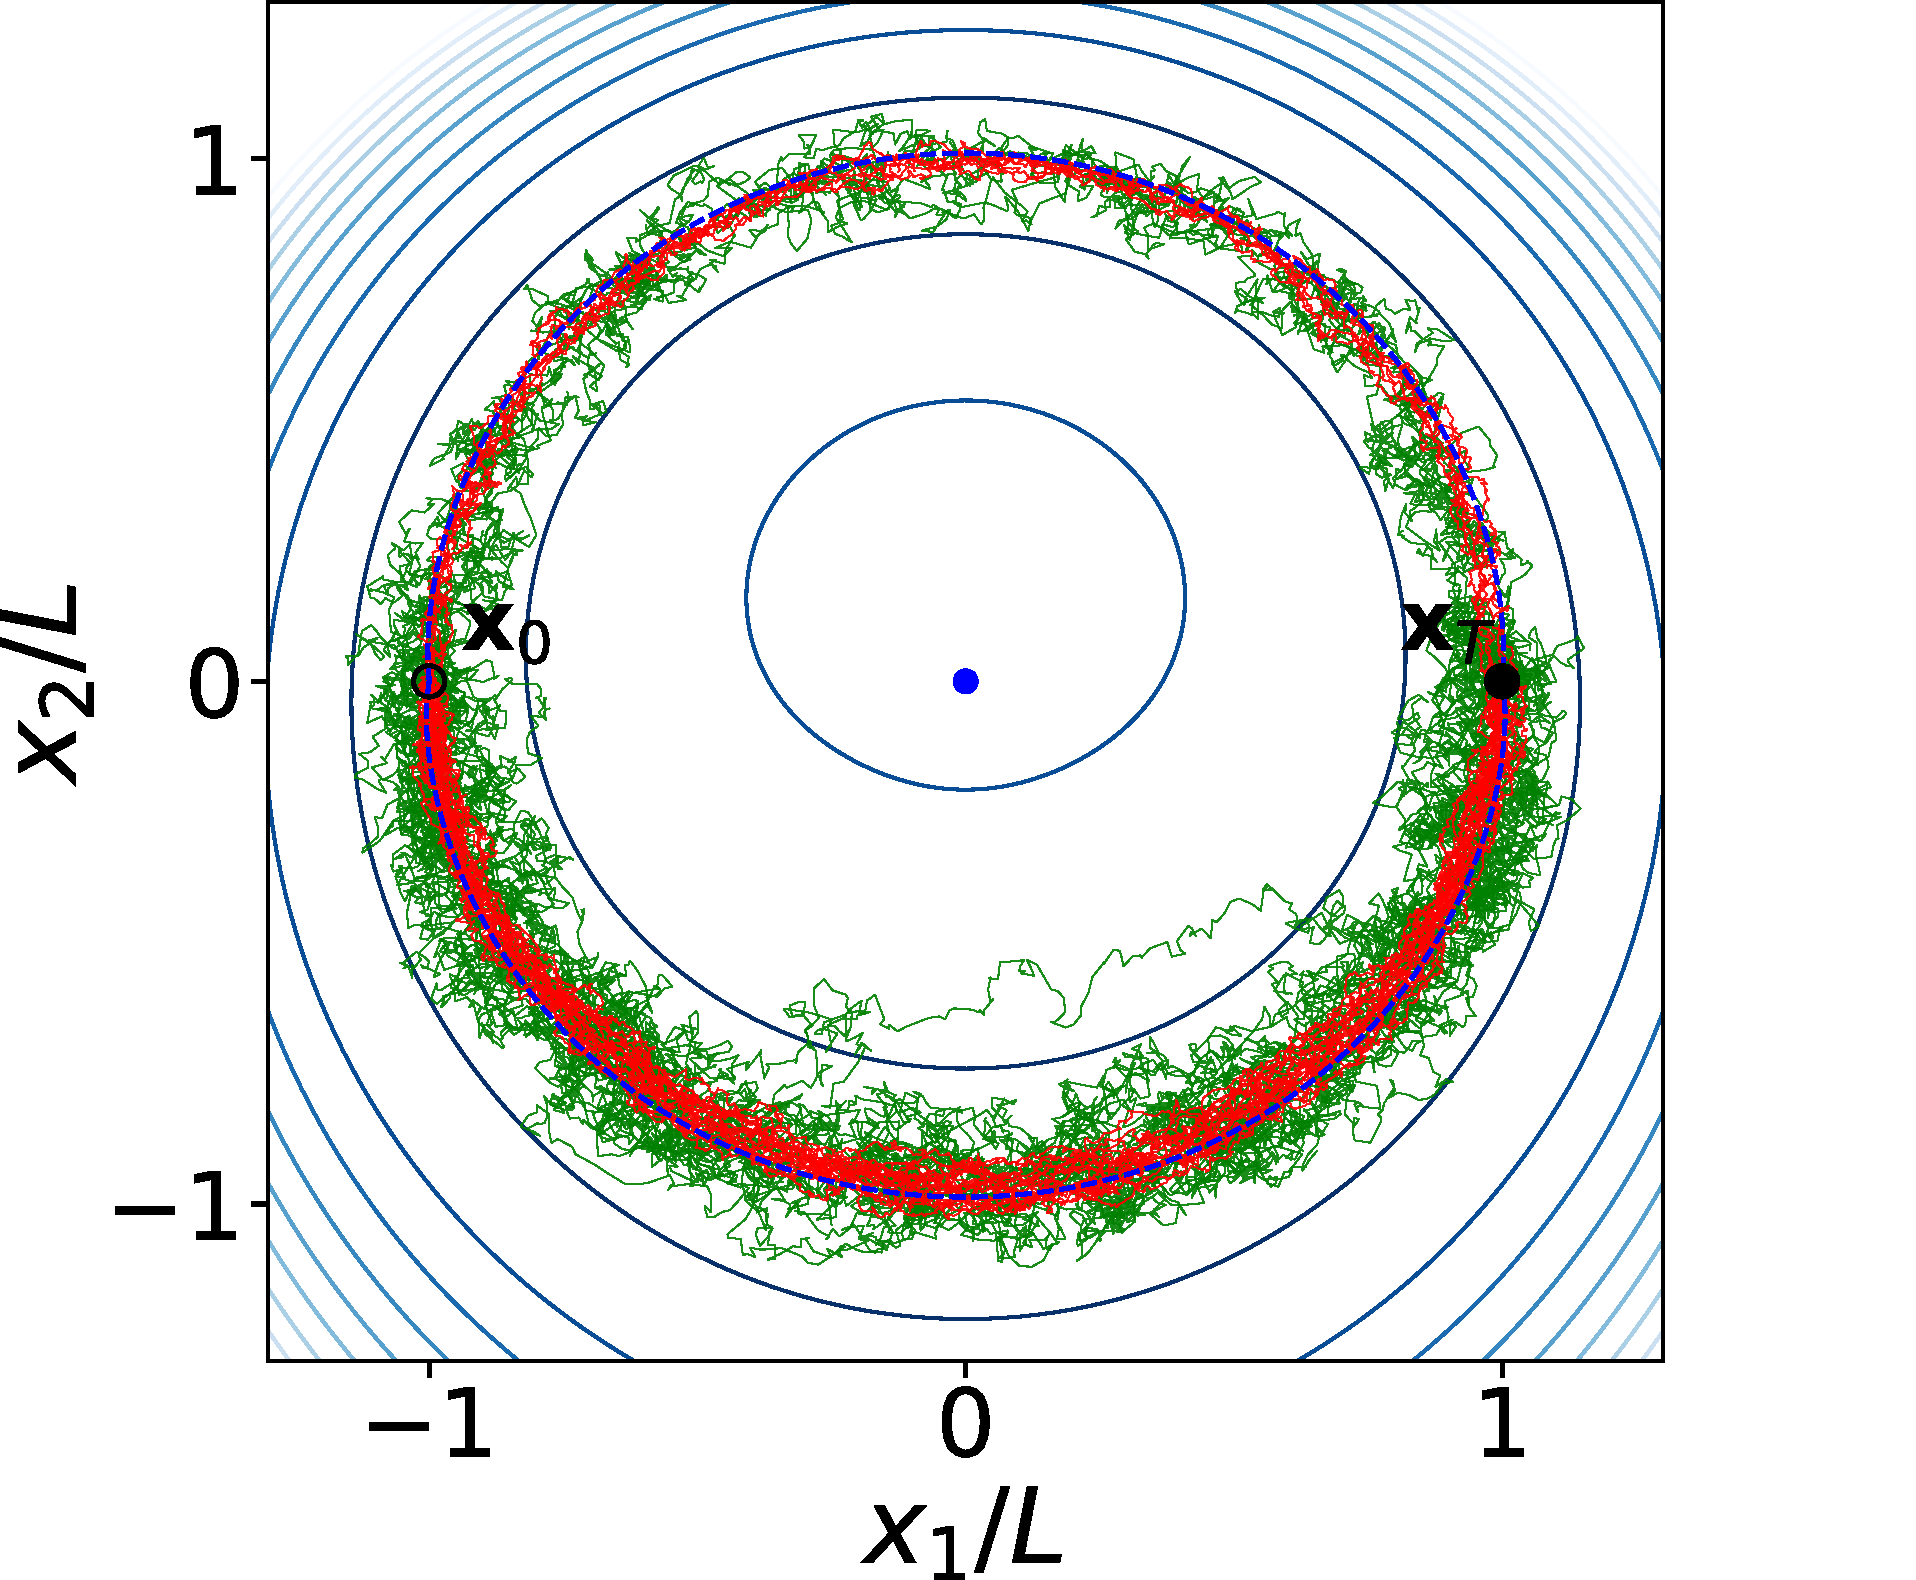
\includegraphics[width=\textwidth]{figs_part1/mcmc/switch_trajectories_without_force}
        \caption[Straight Cosserat rod]%
        {}    
        \label{fig:straight cosserat rod}
    \end{subfigure}
    \hfill
    \begin{subfigure}[b]{0.33\textwidth}
        \centering
        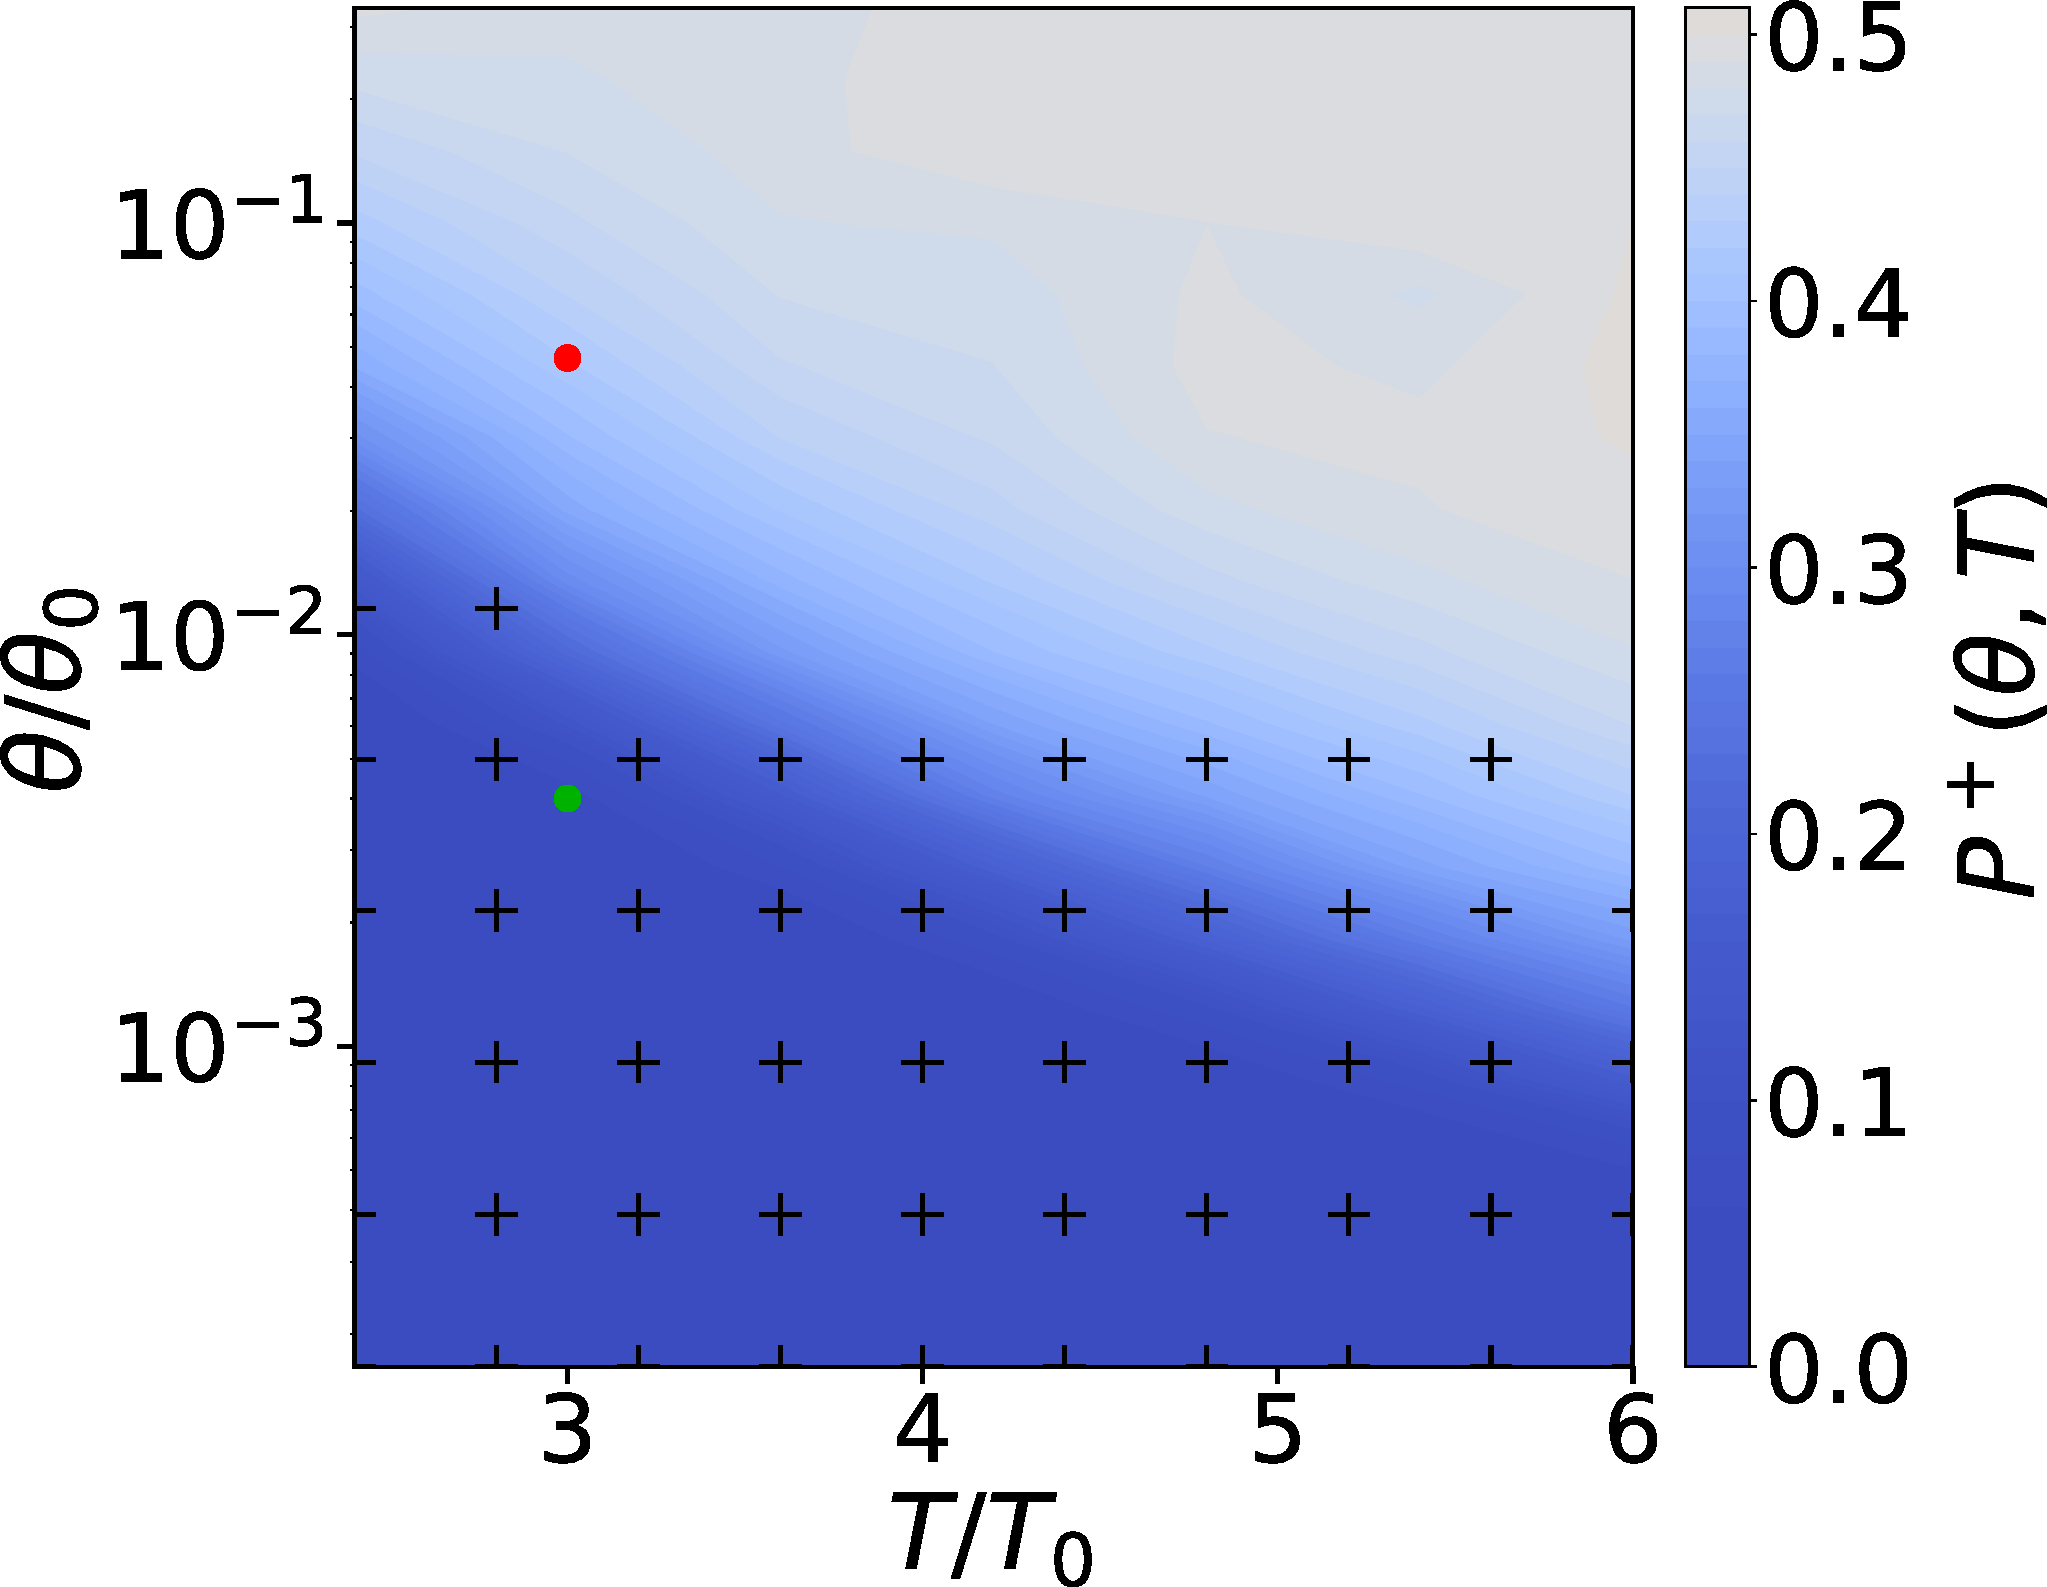
\includegraphics[width=\textwidth]{figs_part1/mcmc/switch_channel_rates}
        \caption[Extending Cosserat rod]%
        {}    
        \label{fig:extending cosserat rod}
    \end{subfigure}    
    \hfill
    \begin{subfigure}[b]{0.314\textwidth}
        \centering
        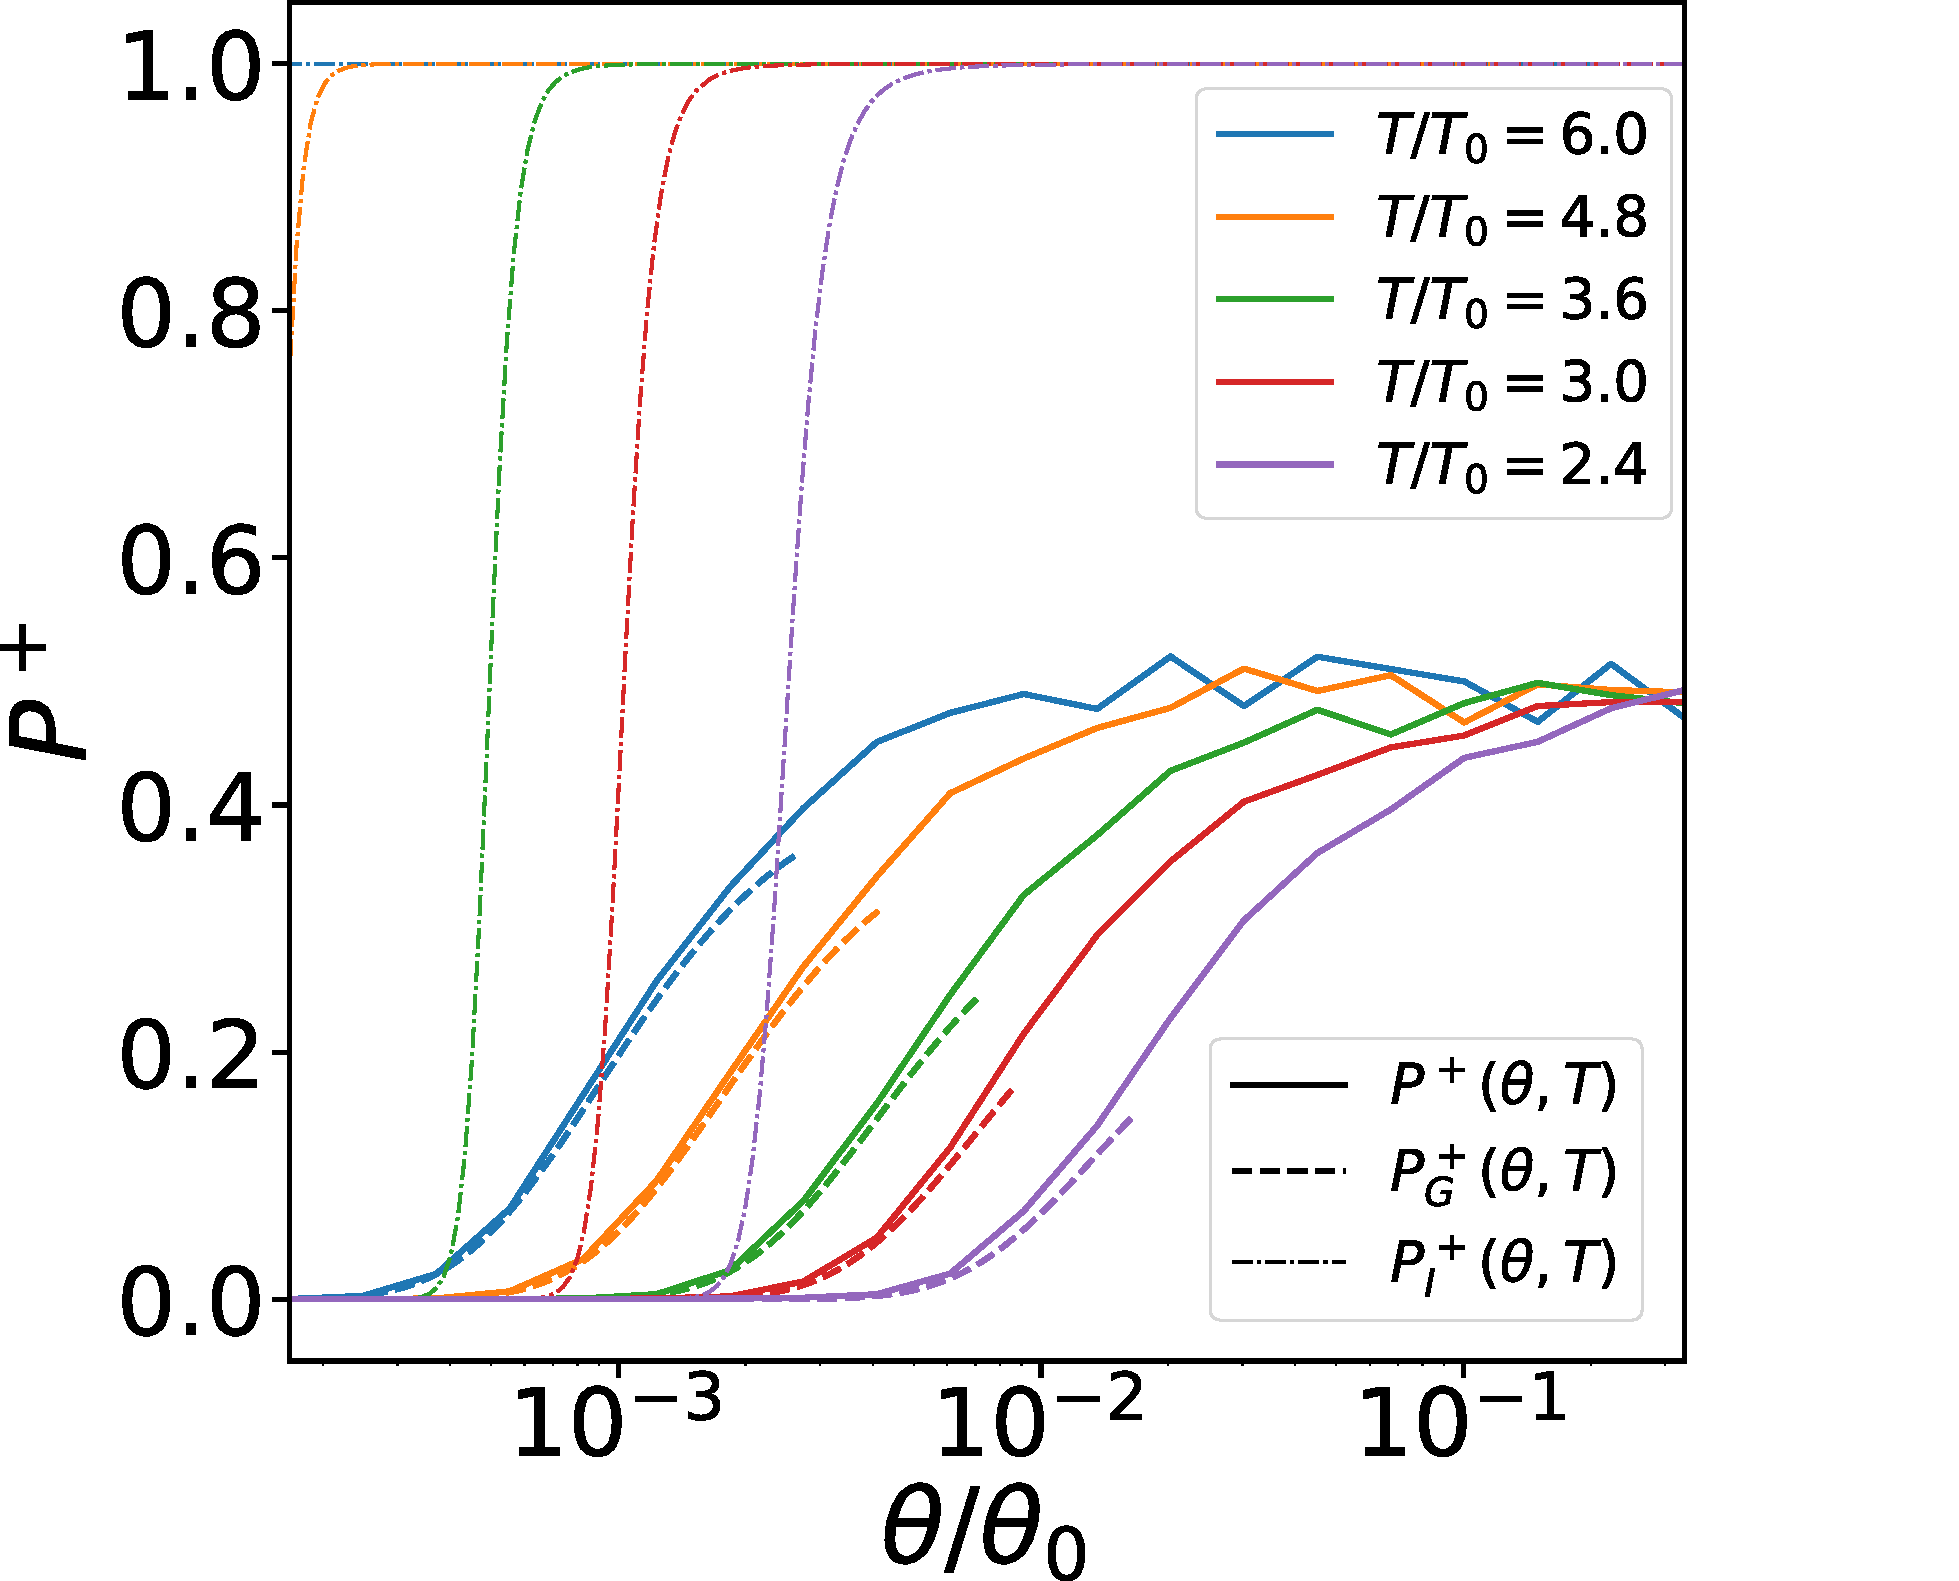
\includegraphics[width=\textwidth]{figs_part1/mcmc/switch_channel_rates_line_plot}
        \caption[Extending Cosserat rod]%
        {}    
        \label{fig:extending cosserat rod}
    \end{subfigure}    
    
    \caption[ The average and standard deviation of critical parameters ]
    {\small Diffusivity-dependence of the transition path ensemble for the conservative
model system. Panel (a) shows 50 stochastic trajectories sampled using
the TMC method (see text) for overdamped dynamics in the potential
$U(x)$ \citep{note:SI}. The dashed blue (green) lines are upper
(lower) instantons between initial (circle, $\mathbf{x}_{0}$) and
final (filled circle, $\mathbf{x}_{T}$) points. Upper and lower channels
are equally populated at temperature $\theta=0.047\theta_{0}$ (green)
but the lower channel is preferred at the lower temperature $\theta=0.004\theta_{0}$
(red). Trajectories of duration $T=3T_{0}$ are sampled with $N=200(T/T_{0})$
modes. Panel (b) is a pseudocolor plot quantifying the variation of
the upper and lower channel probabilites with temperature and duration,
as obtained from TMC. The plus signs show regions where the Gaussian
mixture approximation $P_{G}^{+}$, defined in Eq. (5), is within
a $5\%$ margin of error of the simulated value. The red and green
dots correspond to the same color-coded simulations in panel (a).
Panel (c) shows a comparision between the TMC, Gaussian mixture and
instanton approximations to the upper channel probability as function
of temperature for fixed durations of path.} 
    \label{fig:switch}
\end{figure*} 

\textit{\emph{ To infer the range of
validity of our semi-analytical approximation it is necessary to compare
Eq.~\eqref{eq:r function} with numerical simulations. In parameter
regimes where transitions are very rare, it is not feasible to sample
the TPE using direct simulations. We therefore numerically probe the
TPE using a MCMC algorithm built on the }}\textit{preconditioned Crank-Nicholson
algorithm }\textit{\emph{(pCN) }}\citep{cotterMCMCMethodsFunctions2013,beskosMCMCMETHODSDIFFUSION2008,hairerSpectralGapsMetropolis2014},
as detailed in the SI \citep{note:SI}. In essence, we approximate
the function space of all transition paths by a finite sum of basis
functions \citep{kosambiStatisticsFunctionSpace1943,karhunenUberLineareMethoden1947,loeveProbabilityTheory1977},
and perform a random walk on the resulting finite-dimensional space
of basis coefficients; the random walk is designed such that the resulting
transition path samples are distributed according to the TPE we seek
to probe.

A general shortcoming of MCMC methods and also other transition path
sampling techniques \citep{bolhuisTransitionPathSampling2002,bolhuisTransitionPathSampling,dellagoTransitionPathSampling1998,dellagoEfficientTransitionPath1998a,fujisakiOnsagerMachlupActionbased2010}
is that when the distribution to be sampled is multimodal with regions
of low probability in between the modes, it may take prohibitively
long to obtain converged results. For overdamped Langevin dynamics
Eq.~\eqref{eq:ito equation}, this corresponds to medium-to-low temperature
regimes in systems with competing transition pathways, where the TPE
concentrates around the local instantons. One way to overcome this
issue is to use replica exchange \citep{fujisakiOnsagerMachlupActionbased2010},
which requires running several instances of the MCMC algorithm at
varying temperatures. Here we introduce a modification of the pCN-MCMC
that operates only at one temperature, which we call the \emph{Teleporter
MCMC }(TMC), which utilises the Gaussian mixture approximation of
the TPE. At each step of the TMC there is a small probability to jump
between the transition channels, which accelerates mixing between
them. We provide a detailed description of the algorithm in the SI
\citep{note:SI}.

\section{Results}

We now consider the transition behavior of the 2D
system depicted in Fig.~\ref{fig:switch} (a). For a range of temperatures
$\theta$ and total transition times $T$ we first generate ensembles
of $10^{8}$ sample transition paths per tuple $(\theta,T)$ using
the TMC. Let $\tau_{D}(\theta)=L^{2}/(\mu k_{B}\theta)$, which is
the diffusive time-scale at temperature $\theta$. We also introduce
fixed reference temperature and time-scales $\theta_{0}=U_{0}/k_{B}$
and $T_{0}=\tau_{D}(\theta_{0})$, where $U_{0}$ is the energetic
well-depth of the potential. Our parameter range is such that $T\ll\tau_{D}$,
for each temperature $\theta$ in the range considered. Each sampled
ensemble thus describes a rare transition event. For a total transition
time $T/T_{0}=3$, and for each of the two temperatures $\theta/\theta_{0}=0.047$
and $\theta/\theta_{0}=0.004$, we show 50 randomly chosen TMC sample
paths in Fig.~\ref{fig:switch} (a).  We observe that while for the
higher temperature the paths are evenly distributed between the two
channels, for the lower temperature the lower channel is preferred.
In Fig.~\ref{fig:switch} (b) we show TMC results for $P^{+}(\theta,T)\equiv P^{[1]}(\theta,T)$,
the probability of the upper channel, as a function of both $\theta$
and $T$. Consistent with the $\theta/\theta_{0}=0.047$ data from
Fig.~\ref{fig:switch} (a), we observe that for large enough temperature
$P^{+}(\theta,T)\approx1/2$ (white region), so that upper and lower
channel are equally probable. That at large temperature the asymmetry
in $U$ becomes irrelevant for the TPE is expected, as in this limit
the random force in Eq.~\eqref{eq:ito equation} dominates over the
deterministic force. As $\theta$ is decreased, the channel around
$\Gamma^{-}$ becomes dominant, so that $P^{+}(\theta,T)\rightarrow0$
(blue region in Fig.~\ref{fig:switch} (b), c.f.~$\theta/\theta_{0}=0.004$
data in subplot (a)). The exact temperature at which the crossover
from the diffusivity-dominated regime to the drift-dominated regime
occurs decreases with increasing $T$; this is clearly seen in Fig.~\ref{fig:switch}
(c) where vertical sections of subplot (b) are shown for several values
of $T$.

We now compare our numerical TMC results for $P^{+}(\theta,T)$ with
the Gaussian mixture approximation $P_{G}^{+}(\theta,T)\equiv P_{G}^{[1]}(\theta,T)$,
defined in Eq.~\eqref{eq:r function}. Figure \ref{fig:switch} (b)
shows that this approximation is valid in the low-temperature regime
(plus signs). This is consistent with the assumptions underlying the
Gaussian approximation, as we expect the probability distribution
in path space to be dominated by the neighborhoods of the local instantons
only for sufficiently low temperature. As Fig.~\ref{fig:switch}
(c) shows, $P_{G}^{+}(\theta,T)$ quantitatively captures the beginning
of the crossover from drift-dominated to diffusivity-dominated transition
behaviour for all values of $T$ considered.

For capturing this $\theta$-dependent crossover, the prefactors $\mathcal{Z}^{+}=\mathcal{Z}^{[1]}$,
$\mathcal{Z}^{-}=\mathcal{Z}^{[2]}$ in Eq.~\eqref{eq:r function}
are essential. This becomes apparent by considering $P_{I}^{+}(\theta,T)$,
which only depends on the relative probabilities of the two local
instantons. In Fig.~\ref{fig:switch} (c) we see that for high enough
temperatures $P_{I}^{+}(\theta,T)\approx1$, meaning $S_{\text{OM}}[\mathbf{x}^{+}(t)]<S_{\text{OM}}[\mathbf{x}^{-}(t)]$
\citep{adibStochasticActionsDiffusive2008}. This limit is understood
by comparing the two terms in the action Eq.~\eqref{eq:onsager-machlup action}.
While the first term scales as $1/\theta$, the second term is independent
of $\theta$; for fixed $T$ and large enough $\theta$ the second
term thus dominates the action. This second term is smaller for the
channel around $\Gamma^{+}$ than for the channel around $\Gamma^{-}$,
because the former channel is narrower leading to to a smaller value
of $\nabla\cdot\mathbf{F}$. As $\theta$ is decreased for fixed $T$
the first term in Eq.~\eqref{eq:onsager-machlup action} becomes
dominant. Figure \ref{fig:switch} (c) shows that this leads to a
crossover to $P_{I}^{+}(\theta,T)\approx0$, meaning $\mathbf{x}^{-}$
becomes more probable than $\mathbf{x}^{+}$. While this low-temperature
limit is consistent with the numerical results, the temperature at
which we observe the crossover in $P_{I}^{+}(\theta,T)$ is smaller
as compared to $P^{+}(\theta,T)$. For example, we see in Fig.~\ref{fig:switch}
(c) that for $T/T_{0}=2.4$ the crossover of $P_{I}^{+}(\theta,T)$
is at $\theta/\theta_{0}<10^{-2}$, whereas the crossover for $P^{+}(\theta,T)$
occurs at $\theta/\theta_{0}>10^{-2}$. In particular this implies
that for $\theta/\theta_{0}=10^{-2}$ the most probable path goes
along $\Gamma^{+}$, while most transition paths go along $\Gamma^{-}$.
This highlights that even at intermediate-to-low temperatures, where
the Gaussian mixture approximation Eq.~\eqref{eq:r function} is
already valid, the probabilities of the local instantons alone are
insufficient to obtain the actual transition behaviour. Instead it
is the prefactors $\mathcal{Z^{\pm}}$ in Eq.~\eqref{eq:r function}
that dominate the crossover behaviour in Fig.~\ref{fig:switch} (b);
these Gaussian normalisation constants are, in a sense, an entropic
contribution, as they measure the effective volume in path space of
the support around the respective local instanton. Even though for
$T/T_{0}=2.4$, $\theta/\theta_{0}=10^{-2}$ the instanton $\mathbf{x}^{+}$
is more probable than $\mathbf{x}^{-}$, this is more than offset
by the larger number of paths that behave similar to $\mathbf{x}^{-}$.
As we discuss in the SI \citep{note:SI}, the prefactors $\mathcal{Z^{\pm}}$
remain relevant even in the Freidlin-Wentzell-Graham limit \citep{ventselSMALLRANDOMPERTURBATIONS1970,grahamMacroscopicPotentialsBifurcations1989}
of vanishing temperature and infinite path duration.

\begin{figure}[t]
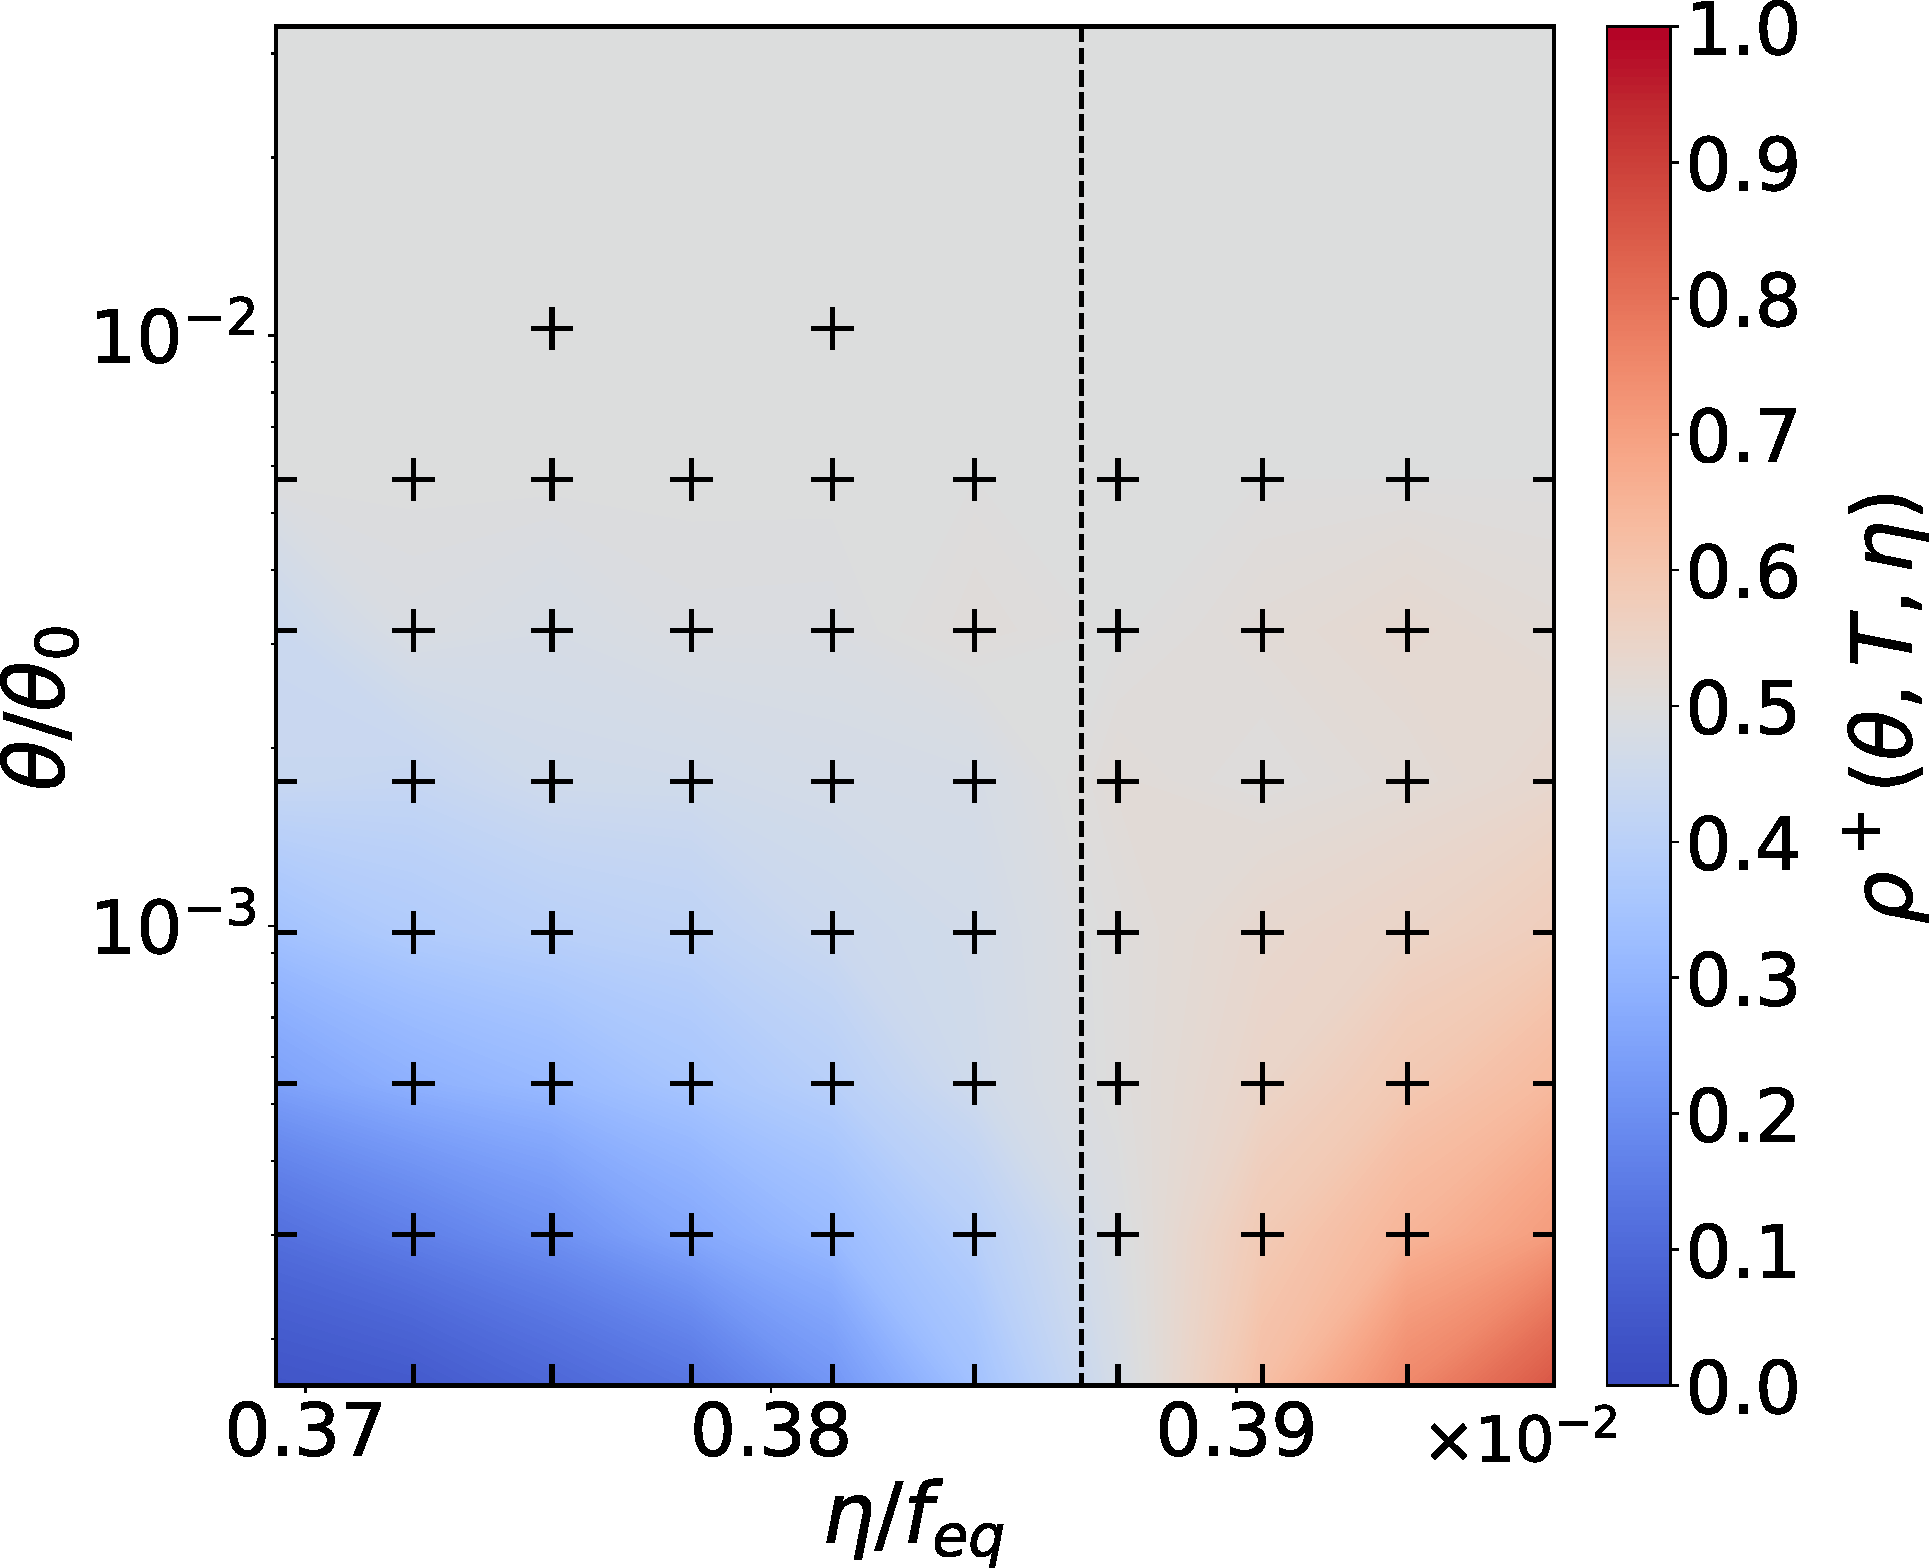
\includegraphics[width=0.36\textwidth]{figs_part1/mcmc/switch_noneq_channel_rates}
\centering \caption{Diffusivity-dependence of the transition path ensemble for the non-conservative
model system. Pseudocolour plot of the probability of the upper channel,
$P^{+}(\theta,T,\eta)$, for the non-gradient system with $T/T_{0}=3$,
as a function of the temperature $\theta$ and the circular force-strength
$\eta$. The black plus signs show regions where the variational approximation
$P_{G}^{+}(\theta,T,\eta)$, defined in Eq. \eqref{eq:r function},
is within a 5\% margin of error of the simulated value. The dashed
line shows the crossover force strength $\eta_{c}/f_{\text{eq}}\approx0.00387$,
where $f_{\text{eq}}$ is the characteristic strength of the gradient
force \citep{note:SI}.}
\label{fig:switch noneq}
\end{figure}

\begin{comment}
As we discuss in the \citep{note:SI}, in the Freidlin-Wentzell-Graham
limit \citep{ventselSMALLRANDOMPERTURBATIONS1970,grahamMacroscopicPotentialsBifurcations1989}
of vanishing temperature and infinite path duration both instantons
become equally probable, $\lim_{T\to\infty}\lim_{\theta\to0}r_{S}(\theta,T)=1/2$.
Nonetheless, also in this limit we expect the TPE to still be entirely
concentrated around $\Gamma^{<}$ because of the unequal normalisation
constants $\mathcal{Z}$ along the two channels \citep{note:SI}.
\end{comment}

For non-gradient forms of the drift, the prefactors $\mathcal{Z^{\pm}}$
can also drive the crossover behaviour of the system, as we show now
by adding a force of strength $\eta$ that acts perpendicular to the
radius vector in the clockwise direction. For positive force strength
$\eta$, this non-conservative force biases towards the upper channel
$\Gamma^{+}$. In Fig.~\ref{fig:switch noneq} we show numerical
results for $P^{+}(\theta,T,\eta)$ as a function of $\eta$ and $\theta$
for $T/T_{0}=3$. For small $\eta/f_{\text{eq}}\rightarrow0$, with
$f_{\text{eq}}$ the characteristic strength of the gradient force
\citep{note:SI}, we recover the results from Fig.~\ref{fig:switch}
(b), (c). Thus at small but finite temperature the dominant transition
channel is the one where particles travel againt the weak non-conservative
force. As $\eta$ is increased to $\eta_{c}/f_{\text{eq}}\approx0.00387$,
we observe a crossover from $\Gamma^{-}$-channel dominated transitions
to $\Gamma^{+}$-channel dominated transitions in the low-temperature
regime. This switch is also captured by the Gaussian approximation
(plus signs in Fig.~\ref{fig:switch noneq}). On the other hand,
throughout the parameter regime considered in Fig.~\ref{fig:switch noneq},
we find that $P_{I}^{+}(\theta,T,\eta)\approx1$, meaning that the
local instanton $\mathbf{x}^{+}$ is always more probable than $\mathbf{x}^{-}$
for finite $\eta$. This again highlights the relevance of considering
Gaussian fluctuations around the instantons for determining the dominant
transition pathway.

\section{Conclusion}

For a system with two competing transition pathways,
we have studied how the dominant transition pathway depends on both
the temperature and the total duration. To quantify the relative importance
of the competing pathways, we have constructed semi-analytical approximators
which are valid in the low-to-intermediate temperature regime. We
have validated our approximators via comparison with a continuous-time
MCMC method that is dimensionally robust and efficiently samples systems
with multiple reactive pathways.

Our results show that even in the low-to-intermediate temperature
regime the global instanton, or most probable path, itself is not
sufficient to determine the dominant transition pathway. Rather, it
is vital that fluctuations around this path be incorporated. This
has a simple one-dimensional equivalent: For a probability density
$\rho(x)\sim\exp(-V(x))$ for some potential $V(x)$ with relative
minima $x_{\alpha}$, the probabilistically most relevant minimum
is not the global one, but that with the largest well probability,
i.e.$~$the $x_{\alpha}$ that maximizes $P(\,\mathrm{well~around~}x_{\alpha}\,)\sim e^{-V(x_{\alpha})}\sqrt{{2\pi}/{V''(x_{\alpha})}}$,
where we use a quadratic Taylor approximation of $V$ around $x_{\alpha}$.
The most probable well is thus determined by an interplay of $e^{-V(x_{\alpha})}$
(which corresponds to the instanton probability $e^{-S_{\text{OM}}[\mathbf{x}^{[\alpha]}]}$)
and $\sqrt{{2\pi}/{V''(x_{\alpha})}}$ (which corresponds to the regularised
normalisation constant $\mathcal{Z}^{[\alpha]}$).

In the present paper we consider a paradigmatic example system with
two competing transition pathways. The method of instantons is an
established technique in theoretical chemistry and statistical physics
\citep{eMinimumActionMethod2004,e_string_2002,grafke_instanton_2015,grafke_numerical_2019,schorleppGelFandYaglomType2021,dematteis_experimental_2019,ferreApproximateOptimalControls2021,kikuchiRitzMethodTransition2020,heymannGeometricMinimumAction2008},
and the method of Gaussian mixtures presented here scales as $O(d^{2})$
with the number of degrees of freedom $d$ \citep{note:SI}. It is
therefore feasible to apply the methods we developed here to more
realistic many-particle systems to study e.g.$~$nucleation pathways
\citep{e_string_2002,lutskoHowCrystalsForm2019,rein_ten_wolde_numerical_1996}
or conformational rearrangements in macromolecules \citep{ren_transition_2005,fujisakiOnsagerMachlupActionbased2010,fujisakiMultiscaleEnhancedPath2013,gartner_modeling_2019}.

Our quantification here of the finite-temperature breakdown of instanton
theories is important for relating such theories to experiments, which
are always at finite temperatures. Our insights into path-space probability
distributions for diffusive stochastic dynamics, together with our
MCMC method, will therefore be valuable for going beyond the regime
of asymptotically low diffusivity in both large deviations theory
\citep{ventselSMALLRANDOMPERTURBATIONS1970,vanden-eijndenGeometricMinimumAction2008,eMinimumActionMethod2004,gartnerModelingSimulationsPolymers2019}
and the study of rare events \citep{grafkeSharpAsymptoticEstimates2021}.
